% !TEX encoding = UTF-8 Unicode
\documentclass[11pt, a4paper, oneside, onecolumn]{ctexart}
\usepackage[utf8]{inputenc}
\usepackage{geometry}
\geometry{left=1.5cm,right=1.5cm,top=2cm,bottom=1cm}
\usepackage{ctex}
\usepackage{CJK}
\usepackage{xcolor}

\usepackage{amsmath, amsthm, amssymb, graphicx, mathrsfs, siunitx,esint}
\usepackage{tikz}
\usepackage{subfigure}
\usepackage{caption}
\usepackage{subcaption}
\usepackage[flushleft]{threeparttable}
\usepackage{cases}

\ctexset{section={format=\bfseries \zihao{4} \flushleft}}
\renewcommand\thesubsection{\thesection.\arabic{subsection}}
\numberwithin{equation}{subsection}
\renewcommand\theequation{\thesubsection.\arabic{equation}}
\makeatletter
\renewcommand{\maketag@@@}[1]{\hbox{\m@th\normalsize\normalfont#1}}%
\makeatother

\usepackage{bookmark}
\usepackage{hyperref}
\hypersetup{colorlinks=true,linkcolor=black}

\usepackage{indentfirst}
\usepackage{inconsolata}

\usepackage{listings}
\lstset{
    basicstyle      =   \zihao{-5}\ttfamily,
    numberstyle     =   \zihao{-5}\ttfamily,
    keywordstyle    =   \color{blue},
    keywordstyle    =   [2] \color{teal},
    stringstyle     =   \color{magenta},
    commentstyle    =   \color{red}\ttfamily,
    breaklines      =   true,   % 自动换行,建议不要写太长的行
    columns         =   fixed,  % 如果不加这一句,字间距就不固定
    flexiblecolumns,                % 别问为什么,加上这个
    numbers             =   left,   % 行号的位置在左边
    showspaces          =   false,  % 是否显示空格,显示了有点乱
    numberstyle         =   \zihao{-5}\ttfamily,    % 行号的样式,小五号,tt 等宽字体
    showstringspaces    =   false,
    captionpos          =   t,      % 这段代码的名字所呈现的位置,t 指的是 top 上面
    frame               =   lrtb,   % 显示边框
}
\lstdefinestyle{Python}{
    language        =   Python, % 语言选 Python
    basicstyle      =   \zihao{-5}\ttfamily,
    numberstyle     =   \zihao{-5}\ttfamily,
    keywordstyle    =   \color{blue},
    keywordstyle    =   [2] \color{teal},
    stringstyle     =   \color{magenta},
    commentstyle    =   \color{red}\ttfamily,
    breaklines      =   true,   % 自动换行,建议不要写太长的行
    columns         =   fixed,  % 如果不加这一句,字间距就不固定
    basewidth       =   0.5em, 
}

% \usepackage{physics} % 物理百宝箱
% \usepackage[version=4]{mhchem} % 绘制分子式
% \usepackage{algorithm,algorithmic} % 展示算法伪代码
% \DeclareMathOperator{\spn}{span}
% \NewDocumentCommand\mathbi{m}{\textbf{\em #1}}

\usepackage[backend=biber]{biblatex}
\addbibresource{/Users/Linyan/Zotero/MyBibTex.bib}

\title{广义相对论基础}
\author{林衍}
\date{\today}

\begin{document}
\maketitle
\subsection*{前言}
本文主要涉及《广义相对论基础》(赵峥、刘文彪)第二章到第四章,《广义相对论引论》(俞允强)第一章到第六章内容,适合本科一二年级阅读。数学前置知识,应该会求导就行了;物理,了解一下拉格朗日方程和变分法就好了,知乎上有不少“一天学完分析力学”,速通一下就行。尽量采用了国际单位制,但缺乏校对精力,还请读者自行确证。

读者们理应了解,根据狭义相对性原理,各惯性系完全等价。但问题是,什么样的参考系是惯性系?地球?地球绕着太阳转动。太阳?太阳绕着银心黑洞转动。狭义相对性原理让表述物理定律时惯性系有优越地位,但自然界却不存在真正的惯性系。因此,爱因斯坦想要将狭义相对性原理推广为广义相对性原理。

然而,如果要等价看待惯性系和非惯性系,势必需要考虑惯性力的问题。我们注意到,惯性力只和物体的质量有关,而引力也有类似的性质。虽然引力质量与惯性质量不同,但各种实验表明二者量级上相同,因此在一个密闭的空间舱中,二者的物理影响不可区分。引力场与惯性场的等效性被称作等效原理。那么在引力场中自由下落的参考系就等价于无引力场太空中的惯性系。这种惯性系在引力场中的其他观测者看来,却是一种在作加速运动的参考系。

惯性力可以通过适当的坐标变换实现,那么引力应当也能,这表明引力来自于时空的几何结构,时空告诉物质如何运动,可以用运动方程来描述。值得注意的是,惯性加速度可以通过坐标系整体的坐标变换消除,但时空各点处的引力往往不同,只能在一点的邻域通过局域的坐标变换消除,因此等效原理是个局域性原理。惯性力和引力还有许多不同,比如惯性力并不起源于物质的相互作用;比如惯性力实际上不改变时空曲率,但引力来自物质,物质会对时空产生内禀效应,物质告诉时空如何弯曲,这对应着爱因斯坦场方程。后来人们证明,可以从爱因斯坦场方程推导出运动方程,引力理论基本方程缩减到一个。

本文首先介绍张量工具和一点黎曼几何,接着研究观测量理论,并阐述广义相对论的基本物理图景。之后将简要介绍球对称度规中引力场的分布和物质的运动。至于黑洞和宇宙学,本文其实是为了《不普通天文学》系列讲义《天体物理基础》写的,会在那里稍作展开。这两部分要深入讲可能会走向《相对论天体物理》或者《宇宙学》,而我现在并没有精力和能力写作,事已至此先这样吧。

\newpage
\tableofcontents

\newpage
\section{数学准备}
\subsection{张量}
一般来讲,观测得到的物理量使用一组数来表示的。而这组数与观测者选定的坐标系相关,比如说火车参考系和地面参考系测得的火车速度不同。然而,尽管同一时空点测量的物理量在不同坐标系会用不同的数组表示,它们本质上描述的是同一个物理量,因此数组的变化应该与坐标变换(即同一时空点在不同坐标系中坐标间的联系)有密切联系。由此可以引出张量的概念。

零阶张量,又被称作标量,是时空坐标的函数。$\widetilde{\boldsymbol{x}}$和$\boldsymbol{x}$是同一时空点在不同坐标系的坐标,但在同一点上测得的物理量应该是一样的,所以标量的值不随广义坐标变换而改变:
\begin{equation}
\widetilde{U}\left(\widetilde{\boldsymbol{x}}\right)=U\left(\boldsymbol{x}\right).
\end{equation}

一阶张量,又被称作向量,可分为逆变向量和协变向量。$n$维空间向量有$n$个分量,每个分量都是时空坐标的函数。向量随坐标变换而变化的规律分别为
\begin{align}
\widetilde{U}^{\mu}&=\frac{\partial{}\widetilde{x}^{\mu}}{\partial{}x^{\nu}}U^{\nu},\\
\widetilde{V}_{\mu}&=\frac{\partial{}{x}^{\nu}}{\partial{}\widetilde{x}^{\mu}}V_{\nu}.
\end{align}
式中已经用到了爱因斯坦求和约定,重复的上下指标需要求和,即$\nu$分别取$0,1,2\cdots$得到的项全部求和。重复指标又称傀儡指标、傀标。逆变向量的指标永远在右上角,协变向量的指标永远在右下角。由于计算可写成矩阵乘法的形式,故$\dfrac{\partial{}\widetilde{x}^{\mu}}{\partial{}x^{\nu}},\dfrac{\partial{}x^{\mu}}{\partial{}\widetilde{x}^{\nu}}$可以看作坐标变换矩阵。每一个时空点都有各自的坐标变换矩阵。我们可以定义 Kroneker 符号$\delta{}^{\mu}_{\nu}$来给出坐标变换矩阵应该满足的关系:
\begin{equation}
\frac{\partial{}\widetilde{x}^{\mu}}{\partial{}x^{\alpha}}\cdot\frac{\partial{}x^{\alpha}}{\partial{}\widetilde{x}^{\nu}}=\delta{}_{\nu}^{\mu}=
\begin{cases}
1,\mu=\nu,\\
0,\mu\ne\nu.
\end{cases}\label{1.1.4}
\end{equation}

一个二阶张量有$n^{2}$个坐标分量,可分为逆变、混合、协变张量,它们随坐标变换而变化,规律分别为
\begin{align}
\widetilde{W}^{\mu\nu}&=\frac{\partial{}\widetilde{x}^{\mu}}{\partial{}x^{\alpha}}\frac{\partial{}\widetilde{x}^{\nu}}{\partial{}x^{\beta}}W^{\alpha\beta},\\
\widetilde{W}^{\mu}_{\nu}&=\frac{\partial{}\widetilde{x}^{\mu}}{\partial{}x^{\alpha}}\frac{\partial{}{x}^{\beta}}{\partial{}\widetilde{x}^{\nu}}W^{\alpha}_{\beta},\\
\widetilde{W}_{\mu\nu}&=\frac{\partial{}{x}^{\alpha}}{\partial{}\widetilde{x}^{\mu}}\frac{\partial{}{x}^{\beta}}{\partial{}\widetilde{x}^{\nu}}W_{\alpha\beta}.
\end{align}
二阶张量的概念可以推广到高阶。拥有$p$个逆变指标和$q$个协变指标的张量称为$\left(p+q\right)$阶混合张量。利用混合张量随坐标变换关系容易证明 Kroneker 符号是个 (1,1) 阶张量,任意坐标系下其形式都为 (\ref{1.1.4}) 式。

多数情况需要研究对称张量。如果高阶张量对一对上标满足
\begin{equation}
T^{\mu\nu\sigma}_{\alpha\beta\gamma\delta{}}=T^{\mu\sigma\nu}_{\alpha\beta\gamma\delta{}},
\end{equation}
则称其对上标$\nu\,\sigma$是对称的。如果
\begin{equation}
T^{\mu\nu\sigma}_{\alpha\beta\gamma\delta{}}=-T^{\mu\sigma\nu}_{\alpha\beta\gamma\delta{}},
\end{equation}
则称其对上标$\nu\,\sigma$是反称的。容易发现两个反称指标取同样值时该分量为 0,比如
\begin{equation}
T^{\mu11}_{\alpha\beta\gamma\delta{}}=-T^{\mu11}_{\alpha\beta\gamma\delta{}}=0,
\end{equation}
对于下标对称和反称的定义是类似的。

对称性仅存在于上标和上标之间,下标和下标之间。如果不具体指明指标,而是直接称某个高阶张量为对称或反对称张量,则它任意两个上标(下标)之间都是对称或反称的。特别地,二阶逆变(协变)张量只有一对上标(下标),如果指标是对称的,根据定义可直接称其为对称张量。反对称亦然。

值得注意的是,任何一个二阶逆变(协变)张量都可以分解成一个对称张量和反对称张量之和:
\begin{equation}
T_{ij}=\frac{1}{2}\left(T_{ij}+T_{ji}\right)+\frac{1}{2}\left(T_{ij}-T_{ji}\right).
\end{equation}

张量加减定义为对应分量的加减,因此作加减运算的张量必须同阶。

张量的乘法叫外乘,作外乘运算的张量不一定要同阶。外乘使张量的阶数升高,如$C_{\alpha\beta\gamma}^{\mu\nu}=A_{\alpha\beta}^{\mu}\cdot B_{\gamma}^{\nu}$.一个$\left(p_{1},q_{1}\right)$阶张量和一个$\left(p_{2},q_{2}\right)$张量相乘,结果是一个$\left(p_{1}+p_{2},q_{1}+q_{2}\right)$阶张量。

混合张量有一种特殊的运算叫作缩并。它让混合张量的⼀对上下标成为重复指标并求和。容易验证,缩并使张量的阶降低。缩并只能在上下标间进行,一个$\left(p,q\right)$阶张量通过缩并变成$\left(p-1,q-1\right)$阶张量。

一个逆变向量和一个协变向量间可以进行内积运算,它的定义是它们外乘后再缩并。以$\left(1,1\right)$阶张量缩并为例,容易发现缩并后变成了标量。
\begin{equation}
C=A^{\mu}B_{\mu}.
\end{equation}

\subsection{平移和联络}
每个时空点的坐标变换都不同,张量分量本身也是时空坐标的函数,因此张量是逐点定义的。两个不同点上的张量直接相减,其差将会失去张量的变换性质,不再是张量。然⽽,研究张量场的微分,又必须⽤到相邻两点的张量之差。为了使微分运算不破坏张量性质,必须⽤⼀种特殊的⽅式来定义相邻两点的张量之差,使新定义的“差”保持张量的变换性质。为此,我们引⼊“⽮量平移”和“仿射联络”两个新概念。

先来研究协变矢量的平移。记矢量场$A_{\mu}$在$P$点的值为$A_{\mu}\left(P\right)$,将其平移到相邻的$Q$点,得到的新矢量记作$A_{\mu}\left(P\to Q\right)$. $A_{\mu}\left(P\right)$在$Q$点无法进行协变变换,但$A_{\mu}\left(P\to Q\right)$可以,因此后者相对前者会多一个增量。这个增量正比于矢量本身和位移$\mathrm{d}x^{\mu}$,满足
\begin{equation}
\delta{}A_{\mu}\left(P\right)=A_{\mu}\left(P\to Q\right)-A_{\mu}\left(P\right)=\Gamma_{\mu\nu}^{\lambda}\left(P\right)\cdot A_{\lambda}\left(P\right)\cdot \mathrm{d}x^{\nu}.\label{1.2.1}
\end{equation}
$\Gamma_{\mu\nu}^{\lambda}\left(P\right)$被称作$P$点的仿射联络,简称联络。根据指标发现四维空间的联络有$4^{3}$个分量。

联络不是张量,我们需要求解联络在坐标变换下的性质。首先从$P$点平移到$Q$的矢量必须是$Q$点处的协变张量
\begin{equation}
\widetilde{A}_{\mu}\left(P\to Q\right)=\left(\frac{\partial{}x^{\alpha}}{\partial{}\widetilde{x}^{\mu}}\right)_{Q}A_{\alpha}\left(P\to Q\right).\label{1.2.2}
\end{equation}
其中变换矩阵须满足微分关系:
\begin{align}
\left(\frac{\partial{}x^{\alpha}}{\partial{}\widetilde{x}^{\mu}}\right)_{Q}&=\left(\frac{\partial{}x^{\alpha}}{\partial{}\widetilde{x}^{\mu}}\right)_{P}+\left(\frac{\partial{}}{\partial{}\widetilde{x}^{\nu}}\left(\frac{\partial{}x^{\alpha}}{\partial{}\widetilde{x}^{\mu}}\right)\right)_{P}\mathrm{d}\widetilde{x}^{\nu}\notag\\
&=\left(\frac{\partial{}x^{\alpha}}{\partial{}\widetilde{x}^{\mu}}\right)_{P}+\left(\frac{\partial{}^{2}x^{\alpha}}{\partial{}\widetilde{x}^{\nu}\partial{}\widetilde{x}^{\mu}}\frac{\partial{}\widetilde{x}^{\nu}}{\partial{}x^{\sigma}}\right)_{P}\mathrm{d}x^{\sigma}.\label{1.2.3}
\end{align}
将 (\ref{1.2.1})(\ref{1.2.3}) 式代入 (\ref{1.2.2}) 式得到
\begin{equation}
\widetilde{A}_{\mu}+\widetilde{\Gamma}_{\mu\nu}^{\lambda}\cdot\widetilde{A}_{\lambda}\cdot\mathrm{d}\widetilde{x}^{\nu}=\left(\frac{\partial{}x^{\alpha}}{\partial{}\widetilde{x}^{\mu}}+\frac{\partial{}^{2}x^{\alpha}}{\partial{}\widetilde{x}^{\nu}\partial{}\widetilde{x}^{\mu}}\frac{\partial{}\widetilde{x}^{\nu}}{\partial{}x^{\sigma}}\mathrm{d}x^{\sigma}\right)\cdot\left(A_{\alpha}+\Gamma_{\alpha\gamma}^{\beta}\cdot A_{\beta}\cdot\mathrm{d}x^{\gamma}\right).
\end{equation}
这些量都是在$P$点处定义的量,所以省略了记号${}_{P}$.而在$P$点处满足
\begin{equation}
\widetilde{A}_{\mu}=\frac{\partial{}x^{\alpha}}{\partial{}\widetilde{x}^{\mu}}A_{\alpha},\mathrm{d}\widetilde{x}^{\nu}=\frac{\partial{}\widetilde{x}^{\nu}}{\partial{}x^{\sigma}}\mathrm{d}x^{\sigma},
\end{equation}
代入上式,略去坐标微分$\mathrm{d}x^{\alpha}$二阶以上小量,
\begin{align}
\frac{\partial{}x^{\alpha}}{\partial{}\widetilde{x}^{\mu}}A_{\alpha}+\widetilde{\Gamma}_{\mu\nu}^{\lambda}\cdot\frac{\partial{}x^{\rho}}{\partial{}\widetilde{x}^{\lambda}}A_{\rho}\cdot\frac{\partial{}\widetilde{x}^{\nu}}{\partial{}x^{\sigma}}\mathrm{d}x^{\sigma}&=\left(\frac{\partial{}x^{\alpha}}{\partial{}\widetilde{x}^{\mu}}+\frac{\partial{}^{2}x^{\alpha}}{\partial{}\widetilde{x}^{\nu}\partial{}\widetilde{x}^{\mu}}\frac{\partial{}\widetilde{x}^{\nu}}{\partial{}x^{\sigma}}\mathrm{d}x^{\sigma}\right)\cdot\left(A_{\alpha}+\Gamma_{\alpha\gamma}^{\beta}\cdot A_{\beta}\cdot\mathrm{d}x^{\gamma}\right).\notag\\
\widetilde{\Gamma}_{\mu\nu}^{\lambda}\cdot\frac{\partial{}x^{\rho}}{\partial{}\widetilde{x}^{\lambda}}A_{\rho}\cdot\frac{\partial{}\widetilde{x}^{\nu}}{\partial{}x^{\sigma}}\mathrm{d}x^{\sigma}&=\Gamma_{\alpha\gamma}^{\beta}\cdot\frac{\partial{}x^{\alpha}}{\partial{}\widetilde{x}^{\mu}}A_{\beta}\cdot\mathrm{d}x^{\gamma}+\frac{\partial{}^{2}x^{\alpha}}{\partial{}\widetilde{x}^{\nu}\partial{}\widetilde{x}^{\mu}}\frac{\partial{}\widetilde{x}^{\nu}}{\partial{}x^{\sigma}}A_{\alpha}\mathrm{d}x^{\sigma}.\notag
\end{align}
注意重复指标可以任取,可以更换,统一记号得到
\begin{equation}
\left(\widetilde{\Gamma}_{\mu\nu}^{\lambda}\cdot\frac{\partial{}x^{\rho}}{\partial{}\widetilde{x}^{\lambda}}\cdot\frac{\partial{}\widetilde{x}^{\nu}}{\partial{}x^{\sigma}}\right.-\left.\Gamma_{\alpha\sigma}^{\rho}\cdot\frac{\partial{}x^{\alpha}}{\partial{}\widetilde{x}^{\mu}}-\frac{\partial{}^{2}x^{\rho}}{\partial{}\widetilde{x}^{\nu}\partial{}\widetilde{x}^{\mu}}\frac{\partial{}\widetilde{x}^{\nu}}{\partial{}x^{\sigma}}\right)A_{\rho}\mathrm{d}x^{\sigma}=0.\notag
\end{equation}
因为矢量和位移任取,所以括号内的部分为零,于是
\begin{equation}
\widetilde{\Gamma}_{\mu\nu}^{\lambda}\cdot\frac{\partial{}x^{\rho}}{\partial{}\widetilde{x}^{\lambda}}\cdot\frac{\partial{}\widetilde{x}^{\nu}}{\partial{}x^{\sigma}}=\Gamma_{\alpha\sigma}^{\rho}\cdot\frac{\partial{}x^{\alpha}}{\partial{}\widetilde{x}^{\mu}}+\frac{\partial{}^{2}x^{\rho}}{\partial{}\widetilde{x}^{\nu}\partial{}\widetilde{x}^{\mu}}\frac{\partial{}\widetilde{x}^{\nu}}{\partial{}x^{\sigma}}.\notag
\end{equation}
两边同乘$\dfrac{\partial{}\widetilde{x}^{\tau}}{\partial{}x^{\rho}}\dfrac{\partial{}x^{\sigma}}{\partial{}\widetilde{x}^{\gamma}}$,重复指标求和,注意到克罗内克符号,得到不同坐标系中仿射联络变换公式
\begin{equation}
\widetilde{\Gamma}_{\mu\nu}^{\tau}=\Gamma_{\alpha\sigma}^{\rho}\frac{\partial{}x^{\alpha}}{\partial{}\widetilde{x}^{\mu}}\frac{\partial{}x^{\sigma}}{\partial{}\widetilde{x}^{\gamma}}\frac{\partial{}\widetilde{x}^{\tau}}{\partial{}x^{\rho}}+\frac{\partial{}^{2}x^{\rho}}{\partial{}\widetilde{x}^{\mu}\partial\widetilde{x}^{\gamma}}\frac{\partial{}\widetilde{x}^{\tau}}{\partial{}x^{\rho}}.
\end{equation}
对联络的限制仅有此式。理论上可在仿射空间中引入多种联络,两种联络的差是张量。

对于逆变矢量,平移增量为
\begin{equation}
\delta{}A^{\mu}\left(P\right)=A^{\mu}\left(P\to Q\right)-A^{\mu}\left(P\right)=-\Gamma_{\lambda\nu}^{\mu}\left(P\right)\cdot A^{\lambda}\left(P\right)\cdot \mathrm{d}x^{\nu}.
\end{equation}

联络一般非对称,但可以分为对称和反对称部分之和。对称部分满足
\begin{equation}
\Gamma_{\left(\mu\nu\right)}^{\lambda}=\frac{1}{2}\left(\Gamma_{\mu\nu}^{\lambda}+\Gamma^{\lambda}_{\nu\mu}\right),
\end{equation}
是一种联络,称其为对称联络,它不是张量。反称部分
\begin{equation}
\Gamma_{\left[\mu\nu\right]}^{\lambda}=\frac{1}{2}\left(\Gamma_{\mu\nu}^{\lambda}-\Gamma_{\nu\mu}^{\lambda}\right)
\end{equation}
是张量,叫挠率张量。

\subsection{协变微商}
有了矢量平移和仿射联络,我们就可以定义张量场的微商运算。这种运算叫协变微商,能保证微商后的量仍是张量。本节需要区分普通微商和协变微商。对于标量场,普通微商用$U_{,\mu}$来表示
\begin{equation}
U_{,\mu}=\frac{\partial{}U\left(\boldsymbol{x}\right)}{\partial{}x^{\mu}}.
\end{equation}
变换到新参考系,得到
\begin{equation}
\widetilde{U}_{,\mu}=\frac{\partial{}\widetilde{U}\left(\widetilde{\boldsymbol{x}}\right)}{\partial{}\widetilde{x}^{\mu}}=\frac{\partial{}\widetilde{U}\left(\widetilde{\boldsymbol{x}}\right)}{\partial{}x^{\alpha}}\frac{\partial{}x^{\alpha}}{\partial{}\widetilde{x}^{\mu}}=\frac{\partial{}U\left(\boldsymbol{x}\right)}{\partial{}x^{\alpha}}\frac{\partial{}x^{\alpha}}{\partial{}\widetilde{x}^{\mu}}=U_{,\alpha}\frac{\partial{}x^{\alpha}}{\partial{}\widetilde{x}^{\mu}}.
\end{equation}
可见$U_{,\mu}$是协变矢量。标量场的普通微商就是它的协变微商:
\begin{equation}
U_{;\mu}=U_{,\mu}.
\end{equation}

协变矢量的普通微商为
\begin{equation}
A_{\mu,\nu}=\frac{\partial{}A_{\mu}}{\partial{}x^{\nu}}=\lim_{Q\to P}\frac{A_{\mu}\left(Q\right)-A_{\mu}\left(P\right)}{\mathrm{d}x^{\nu}}.
\end{equation}
如前文所言,$A_{\mu}\left(Q\right)-A_{\mu}\left(P\right)$不是张量,协变矢量的协变微商要用平移来定义:
\begin{equation}
A_{\mu;\nu}=\lim_{Q\to P}\frac{A_{\mu}\left(Q\right)-A_{\mu}\left(P\to Q\right)}{\mathrm{d}x^{\nu}}=A_{\mu,\nu}-\Gamma_{\mu\nu}^{\lambda}A_{\lambda}.
\end{equation}
可见$A_{\mu;\nu}$是二阶协变张量。

为了唯一确定其他阶张量的协变微商,规定协变微商满足莱布尼茨法则
\begin{equation}
\left(A_{\cdots\cdots}^{\cdots\cdots}B_{\cdots\cdots}^{\cdots\cdots}\right)_{;\lambda}=\left(A_{\cdots\cdots;\lambda}^{\cdots\cdots}\right)\left(B_{\cdots\cdots}^{\cdots\cdots}\right)+\left(A_{\cdots\cdots}^{\cdots\cdots}\right)\left(B_{\cdots\cdots;\lambda}^{\cdots\cdots}\right).
\end{equation}
以逆变矢量的协变微商为例,注意到标量的协变微商是标量的普通微商:
\begin{align}
\left(A^{\mu}B_{\mu}\right)_{;\lambda}&=\left(A^{\mu}B_{\mu}\right)_{,\lambda},\\
A_{;\lambda}^{\mu}B_{\mu}+A^{\mu}B_{\mu;\lambda}&=A_{,\lambda}^{\mu}B_{\mu}+A^{\mu}B_{\mu,\lambda},\notag
\end{align}
注意到协变矢量的协变微商,以及重复指标任取,得到
\begin{equation}
A_{;\lambda}^{\mu}B_{\mu}=A_{,\lambda}^{\mu}B_{\mu}+A^{\mu}\Gamma_{\mu\lambda}^{\nu}B_{\nu}=A^{\mu}_{,\lambda}B_{\mu}+\Gamma_{\alpha\lambda}^{\mu}A^{\alpha}B_{\mu}.\notag
\end{equation}
由于矢量场$B_{\mu}$任取,可得逆变矢量的协变微商
\begin{equation}
A_{;\nu}^{\mu}=A_{,\nu}^{\mu}+\Gamma_{\lambda\nu}^{\mu}A^{\lambda}.
\end{equation}

对于二阶张量则有
\begin{align}
T_{\mu\nu;\lambda}&=T_{\mu\nu,\lambda}-\Gamma_{\mu\lambda}^{\rho}T_{\rho\nu}-\Gamma_{\nu\lambda}^{\rho}T_{\mu\rho}.\\
T_{;\lambda}^{\mu\nu}&=T_{,\lambda}^{\mu\nu}+\Gamma_{\rho\lambda}^{\mu}T^{\rho\nu}+\Gamma_{\rho\lambda}^{\nu}T^{\mu\rho}.\\
T_{\nu;\lambda}^{\mu}&=T_{\nu,\lambda}^{\mu}+\Gamma_{\rho\lambda}^{\mu}T_{\nu}^{\rho}-\Gamma_{\nu\lambda}^{\rho}T_{\rho}^{\mu}.
\end{align}
因此 Kroneker 符号的协变微商为
\begin{align}
\delta{}_{\nu;\lambda}^{\mu}&=\delta{}_{\nu,\lambda}^{\mu}+\Gamma_{\rho\lambda}^{\mu}\delta{}_{\nu}^{\rho}-\Gamma_{\nu\lambda}^{\rho}\delta{}_{\rho}^{\mu}=\delta{}_{\nu,\lambda}^{\mu}=0.
\end{align}

\subsection{测地线和仿射参量}
平直空间中的直线可以定义为两点之间的短程线,也可定义为线上任意相邻两点的切矢量都相互平行的曲线(自平行线)。利用自平行的性质,可将直线概念推广到仿射空间。

四维空间中曲线的参数方程可写为
\begin{equation}
x^{\mu}=x^{\mu}\left(\lambda\right).
\end{equation}
其中$\lambda$是一个标量性质的参量。

曲线上任意一点切矢量定义为
\begin{equation}
A^{\mu}=\frac{\mathrm{d}x^{\mu}}{\mathrm{d}\lambda}.
\end{equation}
这是一个逆变矢量。设曲线上两邻点$P$和$Q$的坐标分别为$x^{\mu}$和$x^{\mu}+\mathrm{d}x^{\mu}$.为了比较两点的切矢量,必须利用平移操作,将$P$点的切矢量$A^{\mu}\left(P\right)$平移到$Q$点。二者平行意味着
\begin{equation}
\frac{A^{1}\left(Q\right)}{A^{1}\left(P\to Q\right)}=\frac{A^{2}\left(Q\right)}{A^{2}\left(P\to Q\right)}=\frac{A^{3}\left(Q\right)}{A^{3}\left(P\to Q\right)}=\frac{A^{4}\left(Q\right)}{A^{4}\left(P\to Q\right)}=F\left(\lambda+\mathrm{d}\lambda\right).
\end{equation}
其中$F$是参量$\lambda$的函数,$P$点的是$F\left(\lambda\right),Q$点的是$F\left(\lambda+\mathrm{d}\lambda\right)$,容易发现
\begin{equation}
F\left(\lambda+\mathrm{d}\lambda\right)=F\left(\lambda\right)+\frac{\mathrm{d}F}{\mathrm{d}\lambda}\mathrm{d}\lambda=1+\frac{\mathrm{d}F}{\mathrm{d}\lambda}\mathrm{d}\lambda,
\end{equation}
于是记$f\left(\lambda\right)=\dfrac{\mathrm{d}F}{\mathrm{d}\lambda}$,自平行线(测地线)即满足
\begin{equation}
A^{\mu}\left(Q\right)=\left[1+f\left(\lambda\right)\mathrm{d}\lambda\right]\cdot A^{\mu}\left(P\to Q\right).
\end{equation}
根据逆变矢量平移公式和切矢量的微分公式
\begin{align}
A^{\mu}\left(P\to Q\right)&=A^{\mu}\left(P\right)-\Gamma_{\alpha\beta}^{\mu}\left(P\right)\cdot A^{\alpha}\left(P\right)\mathrm{d}x^{\beta}=\frac{\mathrm{d}x^{\mu}}{\mathrm{d}\lambda}-\Gamma_{\alpha\beta}^{\mu}\frac{\mathrm{d}x^{\alpha}}{\mathrm{d}\lambda}\frac{\mathrm{d}x^{\beta}}{\mathrm{d}\lambda}\mathrm{d}\lambda,\\
A^{\mu}\left(Q\right)&=A^{\mu}\left(P\right)+\mathrm{d}A^{\mu}\left(P\right)=\frac{\mathrm{d}x^{\mu}}{\mathrm{d}\lambda}+\frac{\mathrm{d}^{2}x^{\mu}}{\mathrm{d}\lambda^{2}}\mathrm{d}\lambda,
\end{align}
自平行条件保留到$\mathrm{d}\lambda$的一阶小量可写作
\begin{equation}
\frac{\mathrm{d}^{2}x^{\mu}}{\mathrm{d}\lambda^{2}}+\Gamma_{\alpha\beta}^{\mu}\frac{\mathrm{d}x^{\alpha}}{\mathrm{d}\lambda}\frac{\mathrm{d}x^{\beta}}{\mathrm{d}\lambda}=f\left(\lambda\right)\frac{\mathrm{d}x^{\mu}}{\mathrm{d}\lambda}.
\end{equation}
这就是测地线应该满足的微分方程。如果标量参量$\lambda$选得足够好,该方程还能得到简化。引入$\lambda=\lambda\left(\sigma\right)$,利用
\begin{align}
\frac{\mathrm{d}x^{\mu}}{\mathrm{d}\lambda}&=\frac{\mathrm{d}x^{\mu}}{\mathrm{d}\sigma}\cdot\frac{\mathrm{d}\sigma}{\mathrm{d}\lambda},\\
\frac{\mathrm{d}^{2}x^{\mu}}{\mathrm{d}\lambda^{2}}&=\frac{\mathrm{d}^{2}x^{\mu}}{\mathrm{d}\sigma^{2}}\cdot\left(\frac{\mathrm{d}\sigma}{\mathrm{d}\lambda}\right)^{2}+\frac{\mathrm{d}x^{\mu}}{\mathrm{d}\sigma}\cdot\frac{\mathrm{d}^{2}\sigma}{\mathrm{d}\lambda^{2}}.
\end{align}
可得
\begin{equation}
\left(\frac{\mathrm{d}^{2}x^{\mu}}{\mathrm{d}\sigma^{2}}+\Gamma_{\alpha\beta}^{\mu}\frac{\mathrm{d}x^{\alpha}}{\mathrm{d}\sigma}\frac{\mathrm{d}x^{\beta}}{\mathrm{d}\sigma}\right)\cdot\left(\frac{\mathrm{d}\sigma}{\mathrm{d}\lambda}\right)^{2}=\frac{\mathrm{d}x^{\mu}}{\mathrm{d}\sigma}\cdot\left[f\left(\lambda\right)\frac{\mathrm{d}\sigma}{\mathrm{d}\lambda}-\frac{\mathrm{d}^{2}\sigma}{\mathrm{d}\lambda^{2}}\right].
\end{equation}
如果标量参量$\sigma$满足
\begin{equation}
f\left(\lambda\right)\frac{\mathrm{d}\sigma}{\mathrm{d}\lambda}=\frac{\mathrm{d}^{2}\sigma}{\mathrm{d}\lambda^{2}},\label{1.4.12}
\end{equation}
测地线方程可以简化为
\begin{equation}
\frac{\mathrm{d}^{2}x^{\mu}}{\mathrm{d}\sigma^{2}}+\Gamma_{\alpha\beta}^{\mu}\frac{\mathrm{d}x^{\alpha}}{\mathrm{d}\sigma}\frac{\mathrm{d}x^{\beta}}{\mathrm{d}\sigma}=0.
\end{equation}
我们称这样的标量参量$\sigma$为仿射参量。

比较化简前后的测地线方程右端,可以发现当采用仿射参量时,$f\left(\sigma\right)=0$,因此自平行条件简化成
\begin{equation}
A^{\mu}\left(Q\right)=A^{\mu}\left(P\to Q\right),
\end{equation}
即沿着这条曲线,从$P$点处平移到$Q$点的曲线切矢量恰等于$Q$点处的曲线切矢量。

值得注意的是,只需满足 (\ref{1.4.12}) 式的参量都是仿射参量,因此仿射参量作线性变换后的参量$a\sigma+b$也是仿射参量。其中$a,b$是常数。

\subsection{曲率和挠率}
联络的反称部分是个张量。由联络出发还可定义另一个张量,即曲率张量。

对一个给定的协变矢量$A_{\lambda}\left(\boldsymbol{x}\right)$求两次协变微商得到
\begin{align}
A_{\lambda;\mu;\nu}&=\left(A_{\lambda,\mu}-\Gamma_{\lambda\mu}^{\rho}A_{\rho}\right)_{;\nu}\notag\\
&=\left(A_{\lambda,\mu}-\Gamma_{\lambda\mu}^{\rho}A_{\rho}\right)_{,\nu}-\Gamma_{\lambda\nu}^{\sigma}\left(A_{\sigma,\mu}-\Gamma_{\sigma\mu}^{\rho}A_{\rho}\right)-\Gamma_{\mu\nu}^{\sigma}\left(A_{\lambda,\sigma}-\Gamma_{\lambda\sigma}^{\rho}A_{\rho}\right)\notag\\
&=\left(A_{\lambda,\mu,\nu}-\Gamma_{\lambda\mu,\nu}^{\rho}A_{\rho}-\Gamma_{\lambda\mu}^{\rho}A_{\rho,\nu}\right)-\Gamma_{\lambda\nu}^{\sigma}A_{\sigma,\mu}+\Gamma_{\lambda\nu}^{\sigma}\Gamma_{\sigma\mu}^{\rho}A_{\rho}-\Gamma_{\mu\nu}^{\sigma}\left(A_{\lambda,\sigma}-\Gamma_{\lambda\sigma}^{\rho}A_{\rho}\right).
\end{align}
傀标可以随意改变,且注意到最后一项括号中$A_{\lambda,\sigma}-\Gamma_{\lambda\sigma}^{\rho}A_{\rho}=A_{\lambda;\sigma}$,上式可写作
\begin{align}
A_{\lambda;\mu;\nu}&=\left(A_{\lambda,\mu,\nu}-\Gamma_{\lambda\mu,\nu}^{\rho}A_{\rho}-\Gamma_{\lambda\mu}^{\rho}A_{\rho,\nu}\right)-\Gamma_{\lambda\nu}^{\sigma}A_{\sigma,\mu}+\Gamma_{\lambda\nu}^{\sigma}\Gamma_{\sigma\mu}^{\rho}A_{\rho}-\Gamma_{\mu\nu}^{\sigma}A_{\lambda;\sigma}\notag\\
&=\left(A_{\lambda,\mu,\nu}-\Gamma_{\lambda\mu,\nu}^{\rho}A_{\rho}-\Gamma_{\lambda\mu}^{\rho}A_{\rho,\nu}\right)-\Gamma_{\lambda\nu}^{\rho}A_{\rho,\mu}+\Gamma_{\lambda\nu}^{\sigma}\Gamma_{\sigma\mu}^{\rho}A_{\rho}-\Gamma_{\mu\nu}^{\rho}A_{\lambda;\rho}.
\end{align}

交换微商顺序,得到
\begin{equation}
A_{\lambda;\nu;\mu}=\left(A_{\lambda,\nu,\mu}-\Gamma_{\lambda\nu,\mu}^{\rho}A_{\rho}-\Gamma_{\lambda\nu}^{\rho}A_{\rho,\mu}\right)-\Gamma_{\lambda\mu}^{\rho}A_{\rho,\nu}+\Gamma_{\lambda\mu}^{\sigma}\Gamma_{\sigma\nu}^{\rho}A_{\rho}-\Gamma_{\nu\mu}^{\rho}A_{\lambda;\rho}.
\end{equation}
二者作差得到
\begin{align}
A_{\lambda;\mu;\nu}-A_{\lambda;\nu;\mu}&=\left(\Gamma_{\lambda\nu,\mu}^{\rho}-\Gamma_{\lambda\mu,\nu}^{\rho}+\Gamma_{\lambda\nu}^{\sigma}\Gamma_{\sigma\mu}^{\rho}-\Gamma_{\lambda\mu}^{\sigma}\Gamma_{\sigma\nu}^{\rho}\right)A_{\rho}+\left(\Gamma_{\nu\mu}^{\rho}-\Gamma_{\mu\nu}^{\rho}\right)A_{\lambda;\rho}\notag\\
&=R_{\lambda\mu\nu}^{\rho}A_{\rho}-2\Gamma^{\rho}_{\left[\mu\nu\right]}A_{\lambda;\rho}.\label{1.5.4}
\end{align}
该式左侧是张量,右侧与挠率张量$\Gamma^{\rho}_{\left[\mu\nu\right]}$有关的那一项也是张量,因此$R_{\lambda\mu\nu}^{\rho}$也必然是张量,我们称其为曲率张量。观察 (\ref{1.5.4}) 式发现曲率张量后一对指标反称,因此只有一二、一三两种独立缩并。

挠率的几何意义是什么呢?考虑自$O$点出发有两个小位移$OQ$和$OQ'$,将$OQ$平移到$Q'P',OQ'$平移到$QP$,如图\ref{挠率的几何意义。}所示。
\begin{figure}[!htp]
\centering
\tikzset{every picture/.style={line width=0.75pt}}
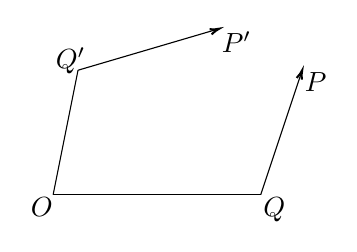
\begin{tikzpicture}[x=0.5pt,y=0.5pt,yscale=0.6,xscale=0.6]
\draw (0,0) -- (30,150) ;
\draw (30,150) -- (200,200) ;
\draw [shift={(200,200)},rotate=-160][line width=0.75](10.93,-3.29) .. controls (6.95,-1.4) and (3.31,-0.3) .. (0,0) .. controls (3.31,0.3) and (6.95,1.4) .. (10.93,3.29); 
\draw (0,0) -- (250,0) ;
\draw (250,0) -- (300,150) ;
\draw [shift={(300,150)},rotate=-109][line width=0.75](10.93,-3.29) .. controls (6.95,-1.4) and (3.31,-0.3) .. (0,0) .. controls (3.31,0.3) and (6.95,1.4) .. (10.93,3.29); 
%Text
\draw (0,180) node [anchor=north west][inner sep=0.75pt]   [align=left] {$Q'$};
\draw (-30,0) node [anchor=north west][inner sep=0.75pt]   [align=left] {$O$};
\draw (250,0) node [anchor=north west][inner sep=0.75pt]   [align=left] {$Q$};
\draw (300,150) node [anchor=north west][inner sep=0.75pt]   [align=left] {$P$};
\draw (200,200) node [anchor=north west][inner sep=0.75pt]   [align=left] {$P'$};
\end{tikzpicture}
\captionsetup{justification=raggedright, singlelinecheck=false}
\caption{挠率的几何意义。}
\label{挠率的几何意义。}
\end{figure}

简单计算平移可得
\begin{align}
OQ&=\mathrm{d}x^{\mu},Q'P'=\mathrm{d}x^{\mu}-\Gamma_{\lambda\nu}^{\mu}\mathrm{d}x^{\lambda}\delta{}x^{\nu},\\
OQ'&=\delta{}x^{\mu},QP=\delta{}x^{\mu}-\Gamma_{\nu\lambda}^{\mu}\delta{}x^{\nu}\mathrm{d}x^{\lambda},\\
PP'&=OQ'+QP'-OQ-QP=\left(\Gamma_{\nu\lambda}^{\mu}-\Gamma_{\lambda\nu}^{\mu}\right)\mathrm{d}x^{\lambda}\delta{}x^{\nu}=2\Gamma^{\mu}_{\left[\nu\lambda\right]}\mathrm{d}x^{\lambda}\delta{}x^{\nu}.
\end{align}
可见挠率为零时才构成封闭的四边形。我们称有挠空间是扭曲的。

假设空间无挠,四边形闭合,同样可通过这种平移研究曲率的几何意义。让某个矢量$A^{\mu}$自$O$点开始,平移$\mathrm{d}x^{\mu}$到$Q$点,然后平移$\delta{}x^{\mu}-\Gamma_{\nu\lambda}^{\mu}\delta{}x^{\nu}\mathrm{d}x^{\lambda}$到$P$点,然后平移$-\left(\mathrm{d}x^{\mu}-\Gamma_{\lambda\nu}^{\mu}\mathrm{d}x^{\lambda}\delta{}x^{\nu}\right)$到$Q'$点,最后平移$-\delta{}x^{\mu}$回到$O$点。在无挠空间中,最后平移得到的结果和原矢量也不一定重合,逐步计算平移可以得到差额,注意计算中要考虑联络随位移的变化。最后(注意无挠空间要求联络对称)结果为
\begin{equation}
\delta{}A^{\mu}=R^{\mu}_{\lambda\nu\gamma}A^{\lambda}\delta{}x^{\nu}\mathrm{d}x^{\gamma}.
\end{equation}
即任意矢量沿无穷小闭合环路平移一周后也必须再附加一个转动才能与原矢量重合。我们称有曲空间是弯曲的。

挠率和曲率都是张量,如果某个参考系中它们所有分量都为零,那么在所有参考系中它们所有分量也都为零,此时称空间是平直的。而联络不是张量,我们可以证明在平直空间中一定可以找到一个坐标系,联络在其中的所有分量都为零,但不能说明联络分量在所有坐标系中都为零。即联络可以“无中生有”,但挠率和曲率不行。

\subsection{度规张量}
为了在仿射空间中引入度量,即定义向量的长度、向量间的夹角,需要引入度规张量$g_{\mu\nu}$,之后仿射空间成为广义黎曼空间。黎曼空间中的线元$\mathrm{d}s$可以表示为
\begin{equation}
\mathrm{d}s^{2}=g_{\mu\nu}\mathrm{d}x^{\mu}\mathrm{d}x^{\nu}.
\end{equation}
要求$\mathrm{d}s^{2}$是标量,即与坐标系选取无关。再加上$\mathrm{d}x^{\mu}$是一阶逆变张量,因此$g_{\mu\nu}$是个二阶协变张量。由于$\mathrm{d}x^{\mu}\mathrm{d}x^{\nu}$对称,因此度规张量必定是对称张量,满足
\begin{equation}
g_{\mu\nu}=g_{\nu\mu}.
\end{equation}

一般来说,黎曼空间中的度规分量不是常数 ($g_{\mu\nu,\lambda}\ne0$),如果是,且度规矩阵行列式不为零,根据线性代数知识,一定可以找到一个坐标变换,将二次型$\mathrm{d}s^{2}=g_{\mu\nu}\mathrm{d}x^{\mu}\mathrm{d}x^{\nu}$化成坐标微分的平方和差形式,使度规在该坐标系下分量为
\begin{equation}
g_{\mu\nu}=
\begin{cases}
\pm1,\mu=\nu,\\
0,\mu\ne\nu.
\end{cases}
\end{equation}
该形式被称作度规张量的正则形式,对应坐标系的基叫正交归一基或幺正基。当且仅当黎曼空间平直时才能在全空间将度规变换到正则形式,不过在某一点的邻域(此时度规可看作常数)还是可以看作局域平直的,因此黎曼空间中可以逐点建立局域闵氏坐标系。闵氏度规为
\begin{equation}
\eta_{\mu\nu}=
\begin{pmatrix}
-1 & 0 & 0 & 0\\
0 & 1 & 0 & 0\\
0 & 0 & 1 & 0\\
0 & 0 & 0 & 1\\
\end{pmatrix}.
\end{equation}

若度规张量非对角元都为零,对角元都为正,称其为正定度规。若非对角元都为零,对角元有正有负,称其为不定度规。定义正则形式下,度规分量对角元之和为度规的号差。可见闵可夫斯基空间的号差为 2.

度规张量的所有坐标分量可以组成一个$4\times4$的对称矩阵,它的逆矩阵对应一个二阶逆变张量$g^{\mu\nu}$,应满足
\begin{equation}
g_{\mu\alpha}g^{\alpha\nu}=g^{\nu}_{\mu}=\delta{}_{\mu}^{\nu}=
\begin{cases}
1,\mu=\nu,\\
0,\mu\ne\nu.
\end{cases}
\end{equation}
利用度规和逆变度规张量可建立逆变和协变向量间的一一对应。记与$U^{\mu}$对应的向量为$U_{\mu}$,其对应关系为
\begin{equation}
U_{\mu}=g_{\mu\nu}U^{\nu},U^{\mu}=g^{\mu\nu}U_{\nu},
\end{equation}
即度规张量分量和逆变度规张量可实现指标的升降,这是张量新的性质。联系内积运算,可见通过度规任意一个矢量都可以构造出一个标量,该标量定义为矢量长度的平方,如
\begin{equation}
g_{\alpha\beta}A^{\alpha}A^{\beta}=A^{\alpha}A_{\alpha}=g^{\alpha\beta}A_{\alpha}A_{\beta}.
\end{equation}
对于二阶张量同样有升降
\begin{equation}
U_{\nu}^{\mu}=g_{\nu\alpha}U^{\alpha\mu},U_{\nu}^{\mu}=g^{\mu\alpha}U_{\alpha\nu}.
\end{equation}

值得一提的是,广义相对论中习惯上取$x^{0}$为时间坐标,即
\begin{equation}
x^{\mu}=\left(ct,x,y,z\right).
\end{equation}
计算中时常会将空间部分单独提出来讨论,习惯上用$i,j$作为空间指标,如$g_{ij}$指代的就是空间部分的度规。

\subsection{Christoffel 符号}
引入度量后我们希望矢量长度在平移下保持不变。如果条件再严格一点,采用对称联络(无挠空间),矢量长度平移不变性将唯一确定对称联络和度规张量的关系。首先将$P$点的逆变矢量$A^{\mu}\left(P\right)$平移到邻近点$Q$,可知
\begin{equation}
A^{\mu}\left(P\to Q\right)=A^{\mu}\left(P\right)-\Gamma_{\nu\lambda}^{\mu}\left(P\right)A^{\nu}\left(P\right)\mathrm{d}x^{\lambda}.\label{1.7.1}
\end{equation}

两点间的度规张量满足
\begin{equation}
g_{\mu\nu}\left(Q\right)=g_{\mu\nu}\left(P\right)+g_{\mu\nu,\lambda}\left(P\right)\cdot\mathrm{d}x^{\lambda}.\label{1.7.2}
\end{equation}
平移不改变矢量长度,则有
\begin{equation}
g_{\mu\nu}\left(Q\right)A^{\mu}\left(P\to Q\right)A^{\nu}\left(P\to Q\right)=g_{\mu\nu}\left(P\right)A^{\mu}\left(P\right)A^{\nu}\left(P\right).\label{1.7.3}
\end{equation}

将 (\ref{1.7.1})(\ref{1.7.2}) 式代入 (\ref{1.7.3}) 式,并略去$\mathrm{d}x^{\mu}$二阶以上小量,可得
\begin{equation}
\left(g_{\mu\nu,\lambda}-g_{\alpha\nu}\Gamma_{\mu\lambda}^{\alpha}-g_{\mu\alpha}\Gamma_{\nu\lambda}^{\alpha}\right)A^{\mu}A^{\nu}\mathrm{d}x^{\lambda}=0.
\end{equation}
注意到$A^{\mu}$是任意矢量,$\mathrm{d}x^{\lambda}$是任意位移,括号内为零。轮换指标可得
\begin{align}
g_{\mu\nu,\lambda}-g_{\alpha\nu}\Gamma_{\mu\lambda}^{\alpha}-g_{\mu\alpha}\Gamma_{\nu\lambda}^{\alpha}=0,\label{1.7.5}\\
g_{\nu\lambda,\mu}-g_{\alpha\lambda}\Gamma_{\nu\mu}^{\alpha}-g_{\nu\alpha}\Gamma_{\lambda\mu}^{\alpha}=0.\label{1.7.6}\\
g_{\lambda\mu,\nu}-g_{\alpha\mu}\Gamma_{\lambda\nu}^{\alpha}-g_{\alpha\alpha}\Gamma_{\mu\nu}^{\alpha}=0.\label{1.7.7}
\end{align}
(\ref{1.7.6})(\ref{1.7.7}) 式相加再减去 (\ref{1.7.5}) 式,并注意到无挠空间联络的对称性,可以得到
\begin{align}
\Gamma_{\lambda\mu\nu}&=g_{\lambda\alpha}\Gamma_{\mu\nu}^{\alpha}=\frac{1}{2}\left(g_{\mu\lambda,\nu}+g_{\nu\lambda,\mu}-g_{\mu\nu,\lambda}\right),\\
\Gamma_{\mu\nu}^{\alpha}&=\frac12g^{\alpha\lambda}\left(g_{\mu\lambda,\nu}+g_{\nu\lambda,\mu}-g_{\mu\nu,\lambda}\right).
\end{align}
于是我们建立了无挠黎曼空间中,保持矢量长度平移不变条件下对称联络与度规的泛函关系式。满足此式的联络称为 Christoffel 联络,简称克氏符。

此外还可注意到 (\ref{1.7.5}) 式等价于度规张量的协变微商为零。可以证明
\begin{align}
g_{\mu\nu;\lambda}=g^{\mu\nu}_{;\lambda}=0.
\end{align}

广义相对论所用的时空是无挠的黎曼时空。前文曾提过无挠的黎曼时空对其中任意一点,都可以找到一个坐标变换,将那点的克氏符的所有分量都变到零。此处可以给出证明。令坐标$x^{\mu}$下$P$点坐标为$x^{\mu}_{P},P$点的联络为$\left(\Gamma^{\lambda}_{\mu\nu}\right)_{P}$,找到坐标变换$x^{\mu}\to\widetilde{x}^{\mu}$,让$P$点在新坐标系中的坐标$\widetilde{x}^{\mu}_{P}=0$,且坐标变换满足
\begin{equation}
x^{\mu}-x^{\mu}_{P}=\widetilde{x}^{\mu}+\frac{1}{2}C_{\alpha\beta}^{\mu}\widetilde{x}^{\alpha}\widetilde{x}^{\beta},
\end{equation}
其中$C_{\alpha\beta}^{\mu}=C_{\beta\alpha}^{\mu}$,分量都是常数。根据上式得到$P$点坐标变换矩阵满足
\begin{equation}
\left(\frac{\partial{}x^{\mu}}{\partial{}\widetilde{x}^{\lambda}}\right)_{P}=\delta{}^{\mu}_{\nu},\left(\frac{\partial{}\widetilde{x}^{\mu}}{\partial{}x^{\lambda}}\right)_{P}=\delta{}^{\mu}_{\lambda},\left(\frac{\partial{}^{2}x^{\mu}}{\partial{}\widetilde{x}^{\lambda}\partial{}\widetilde{x}^{\nu}}\right)_{P}=C_{\lambda\nu}^{\mu},
\end{equation}
将其带入联络变换式得到
\begin{equation}
\left(\widetilde{\Gamma}^{\lambda}_{\mu\nu}\right)_{P}=\left(\Gamma^{\lambda}_{\mu\nu}\right)_{P}+C_{\mu\nu}^{\lambda}.
\end{equation}
因此适当地选取$C_{\mu\nu}^{\lambda}$就可让新坐标系中$P$点联络为零。利用 (\ref{1.7.5}) 式可以看出此时$g_{\mu\nu,\lambda}=0$,即度规在局域内是常数。我们已经知道这意味着可以将度规分量写作正则形式,时空是局域平直的。通过测地线方程很容易看出平直性。我们知道采用仿射参量时测地线方程可以写作
\begin{equation}
\frac{\mathrm{d}^{2}x^{\mu}}{\mathrm{d}\sigma^{2}}+\Gamma_{\alpha\beta}^{\mu}\frac{\mathrm{d}x^{\alpha}}{\mathrm{d}\sigma}\frac{\mathrm{d}x^{\beta}}{\mathrm{d}\sigma}=0,\tag{1.4.13}
\end{equation}
因此克氏符变为零时测地线方程变成直线方程:
\begin{equation}
\frac{\mathrm{d}^{2}x^{\mu}}{\mathrm{d}\sigma^{2}}=0.
\end{equation}
而平直空间中直线运动与惯性运动是相联系的,表明此刻物质不受引力或惯性力,这是个惯性系。从上述论述我们还可发现联络部分就对应着引力场强或惯性场强,而我们总可以在一点通过选择合适的参考系消除联络部分,这便是等效原理的数学基础。值得注意的是,在有挠空间找不到上述坐标变换,等效原理不成立。但实验表明至少在真空处,挠率一定为零,我们的时空是弯曲的,但不是扭曲的。

费米进一步指出,黎曼时空中任一点总可以找到一个沿测地线(物理上可看作在引力场中自由下落)平移(即无转动)的无穷小坐标系,使该点邻域联络所有分量在其中始终为零,这个坐标系即局部惯性系。

\subsection{短程线}
黎曼空间任意两点间可以有无数条连线,取极值为短程线。取极值并不意味着这条线最短,也可能是最长的一条。现在我们用变分原理来求短程线。首先定义泛函
\begin{equation}
S=\int_{A}^{B}\mathrm{d}s,
\end{equation}
积分可沿通过$A,B$的任意曲线来作,$\mathrm{d}s$为线元,则$S$为曲线的“长度”。短程线必须满足
\begin{equation}
\delta{}S=\delta{}\int_{A}^{B}\mathrm{d}s=0.\label{1.8.2}
\end{equation}
线元可以记作
\begin{align}
\mathrm{d}s&=\left(g_{\alpha\beta}\mathrm{d}x^{\alpha}\mathrm{d}x^{\beta}\right)^{\frac12}=\left(g_{\alpha\beta}\frac{\mathrm{d}x^{\alpha}}{\mathrm{d}\lambda}\frac{\mathrm{d}x^{\beta}}{\mathrm{d}\lambda}\right)^{\frac12}\mathrm{d}\lambda\notag\\
&=\left(g_{\alpha\beta}\dot{x}^{\alpha}\dot{x}^{\beta}\right)^{\frac12}\mathrm{d}\lambda=L\mathrm{d}\lambda.
\end{align}
其中$L$是拉格朗日函数。(\ref{1.8.2}) 式改写为
\begin{equation}
\delta{}\int_{A}^{B}L\mathrm{d}\lambda=0.
\end{equation}
其满足的拉格朗日方程为
\begin{align}
\frac{\partial{}L}{\partial{}x^{\mu}}&-\frac{\mathrm{d}}{\mathrm{d}\lambda}\frac{\partial{}L}{\partial{}\dot{x}^{\nu}}=0.\\
\frac{1}{\left(g_{\alpha\beta}\dot{x}^{\alpha}\dot{x}^{\beta}\right)^{\frac12}}\frac{\partial{}g_{\alpha\beta}}{\partial{}x^{\nu}}\dot{x}^{\alpha}\dot{x}^{\beta}&-\frac{\mathrm{d}}{\mathrm{d}\lambda}\frac{g_{\alpha\nu}\dot{x}^{\alpha}+g_{\beta\nu}\dot{x}^{\beta}}{\left(g_{\alpha\beta}\dot{x}^{\alpha}\dot{x}^{\beta}\right)^{\frac12}}=0.\label{1.8.6}
\end{align}
如果标量参量$\lambda$为线长$\mathrm{d}s$,则有
\begin{equation}
\left(g_{\alpha\beta}\dot{x}^{\alpha}\dot{x}^{\beta}\right)^{\frac12}=g_{\alpha\beta}\frac{\mathrm{d}x^{\alpha}}{\mathrm{d}\lambda}\frac{\mathrm{d}x^{\beta}}{\mathrm{d}\lambda}=g_{\alpha\beta}\frac{\mathrm{d}x^{\alpha}}{\mathrm{d}s}\frac{\mathrm{d}x^{\beta}}{\mathrm{d}s}=1,
\end{equation}
(\ref{1.8.6}) 式可以写作
\begin{align}
&g_{\alpha\beta,\nu}\dot{x}^{\alpha}\dot{x}^{\beta}-2\frac{\mathrm{d}}{\mathrm{d}s}\left(g_{\alpha\nu}\dot{x}^{\alpha}\right)=0,\notag\\
&g_{\alpha\nu}\frac{\mathrm{d}^{2}x^{\alpha}}{\mathrm{d}s^{2}}+\left(g_{\alpha\nu,\beta}-\frac12g_{\alpha\beta,\nu}\right)\frac{\mathrm{d}x^{\alpha}}{\mathrm{d}s}\frac{\mathrm{d}x^{\beta}}{\mathrm{d}s}=0.\label{1.8.8}
\end{align}
注意到
\begin{equation}
g_{\alpha\nu,\beta}\frac{\mathrm{d}x^{\alpha}}{\mathrm{d}s}\frac{\mathrm{d}x^{\beta}}{\mathrm{d}s}=g_{\beta\nu,\alpha}\frac{\mathrm{d}x^{\beta}}{\mathrm{d}s}\frac{\mathrm{d}x^{\alpha}}{\mathrm{d}s}=g_{\beta\nu,\alpha}\frac{\mathrm{d}x^{\alpha}}{\mathrm{d}s}\frac{\mathrm{d}x^{\beta}}{\mathrm{d}s},
\end{equation}
(\ref{1.8.8}) 式可以写作
\begin{equation}
g_{\mu\nu}\frac{\mathrm{d}^{2}x^{\mu}}{\mathrm{d}s^{2}}+\frac12\left[g_{\alpha\nu,\beta}+g_{\beta\nu,\alpha}-g_{\alpha\beta,\nu}\right]\frac{\mathrm{d}x^{\alpha}}{\mathrm{d}s}\frac{\mathrm{d}x^{\beta}}{\mathrm{d}s}=0,
\end{equation}
即
\begin{equation}
\frac{\mathrm{d}^{2}x^{\mu}}{\mathrm{d}s^{2}}+\Gamma_{\alpha\beta}^{\mu}\frac{\mathrm{d}x^{\alpha}}{\mathrm{d}s}\frac{\mathrm{d}x^{\beta}}{\mathrm{d}s}=0.
\end{equation}
即短程线方程与测地线方程完全一样。不过短程线中的联络必须是克氏符,测地线则不一定,测地线可以在有挠时空中成立。仅在挠率为零且联络为克氏符的黎曼空间中测地线才是短程线。沿测地线的距离参量可以选作测地线的仿射参量,但对于光来讲,其走过长度始终为零,要选择其他的仿射参量。

\subsection{曲率张量}
本节具体讨论无挠且矢量长度平移不变的黎曼空间中曲率张量的性质。

首先曲率张量与联络关系为
\begin{equation}
R_{\lambda\mu\nu}^{\rho}=\Gamma_{\lambda\nu,\mu}^{\rho}-\Gamma_{\lambda\mu,\nu}^{\rho}+\Gamma_{\lambda\nu}^{\sigma}\Gamma_{\sigma\mu}^{\rho}-\Gamma_{\lambda\mu}^{\sigma}\Gamma_{\sigma\nu}^{\rho}.\label{1.9.1}
\end{equation}
此为曲率张量的$(1,3)$型表示,为了进一步研究它的对称性,引入$\left(0,4\right)$型表示
\begin{equation}
R_{\rho\lambda\mu\nu}=g_{\rho\sigma}R^{\sigma}_{\lambda\mu\nu}.\label{1.9.2}
\end{equation}
根据 (\ref{1.9.1}) 式表示容易看出后一对指标是反对称的
\begin{equation}
R_{\lambda\mu\nu}^{\rho}=-R_{\lambda\nu\mu}^{\rho},R_{\rho\lambda\mu\nu}=-R_{\rho\lambda\nu\mu}.\label{1.9.3}
\end{equation}
将 (\ref{1.9.2}) 式联络的微分展开成度规的二阶微分可知前一对指标和后一对指标是对称的
\begin{equation}
R_{\rho\lambda\mu\nu}=R_{\mu\nu\rho\lambda}.\label{1.9.4}
\end{equation}
结合 (\ref{1.9.3})(\ref{1.9.4}) 式可得前一对指标也是反对称的
\begin{equation}
R_{\rho\lambda\mu\nu}=-R_{\lambda\rho\mu\nu}.
\end{equation}
根据 (\ref{1.9.1})(\ref{1.9.2}) 式可以得到 Ricci 恒等式
\begin{equation}
R_{\lambda\mu\nu}^{\rho}+R_{\mu\nu\lambda}^{\rho}+R_{\nu\lambda\mu}^{\rho}=0,R_{\rho\lambda\mu\nu}+R_{\rho\mu\nu\lambda}+R_{\rho\nu\lambda\mu}=0.
\end{equation}
如上四种对称性要求曲率张量只有 20 个独立分量。

接着考虑曲率张量的缩并。克氏符的对称性增加了曲率张量的对称性,此时一二缩并为零,曲率张量仅剩一三独立缩并,得到的张量为 Ricci 张量:
\begin{equation}
R_{\mu\nu}=R^{\lambda}_{\mu\lambda\nu}.
\end{equation}
值得注意的是,完全可以在曲率张量不为零的情况下实现 Ricci 张量为零。

Ricci 张量是对称的
\begin{equation}
R_{\mu\nu}=g^{\lambda\rho}R_{\rho\mu\lambda\nu}=g^{\lambda\rho}R_{\lambda\nu\rho\mu}=g^{\rho\lambda}R_{\lambda\nu\rho\mu}=R^{\rho}_{\nu\rho\mu}=R_{\nu\mu}.
\end{equation}
根据 Ricci 张量可以定义曲率标量
\begin{equation}
R=g^{\mu\nu}R_{\mu\nu}.
\end{equation}
最后定义爱因斯坦张量
\begin{equation}
G_{\mu\nu}=R_{\mu\nu}-\frac12g_{\mu\nu}R.
\end{equation}
在$4$维空间中,$R_{\mu\nu}$有$4^{2}$个分量,由于它是对称张量,因此独立分量个数为$4+\dfrac{16-4}{2}=10$个。可见爱因斯坦张量独立分量也有 10 个。

广义相对论所用的黎曼空间是无挠的。如果在一定时空范围内曲率张量也为零,则一定可以找到一个坐标系使该时空范围内联络所有分量都为零(与等效原理不同,此时不局限于一点邻域),前文提到过这意味着空间是平坦的。因此
\begin{equation}
R_{\lambda\mu\nu}^{\rho}=0,
\end{equation}
是空间平坦性的判据。

根据 (\ref{1.9.1}) 式出发还可证明 Bianchi 恒等式。选取联络为零的坐标系可得
\begin{align}
R^{\rho}_{\lambda\mu\nu;\sigma}=\left(\Gamma^{\rho}_{\lambda\nu,\mu}-\Gamma_{\lambda\mu,\nu}^{\rho}\right)_{,\sigma}=\Gamma^{\rho}_{\lambda\nu,\mu,\sigma}-\Gamma^{\rho}_{\lambda\mu,\nu,\sigma},\\
R^{\rho}_{\lambda\nu\sigma;\mu}=\left(\Gamma^{\rho}_{\lambda\sigma,\nu}-\Gamma_{\lambda\nu,\sigma}^{\rho}\right)_{,\mu}=\Gamma^{\rho}_{\lambda\sigma,\nu,\mu}-\Gamma^{\rho}_{\lambda\nu,\sigma,\mu},\\
R^{\rho}_{\lambda\sigma\mu;\nu}=\left(\Gamma^{\rho}_{\lambda\mu,\sigma}-\Gamma_{\lambda\sigma,\mu}^{\rho}\right)_{,\nu}=\Gamma^{\rho}_{\lambda\mu,\sigma,\nu}-\Gamma^{\rho}_{\lambda\sigma,\mu,\nu}.
\end{align}
注意到普通微商顺序可交换,得到 Bianchi 恒等式:
\begin{equation}
R^{\rho}_{\lambda\mu\nu;\sigma}+R^{\rho}_{\lambda\nu\sigma;\mu}+R^{\rho}_{\lambda\sigma\mu;\nu}=0.
\end{equation}
缩并指标$\rho,\sigma$,注意到反称性,得到
\begin{equation}
R^{\sigma}_{\lambda\mu\nu;\sigma}-R_{\lambda\nu;\mu}+R_{\lambda\mu;\nu}=0.
\end{equation}
乘以$g^{\nu\lambda}$,并注意到$g^{\nu\lambda}_{;\alpha}=0$,得到
\begin{equation}
R^{\sigma}_{\mu;\sigma}-R_{;\mu}+R^{\nu}_{\mu;\nu}=0.
\end{equation}
即
\begin{equation}
R^{\nu}_{\mu;\nu}-\frac12R_{;\mu}=0.
\end{equation}
也即
\begin{equation}
\left(R^{\nu}_{\mu}-\frac12\delta{}_{\mu}^{\nu}R\right)_{;\nu}=0.
\end{equation}
这表明爱因斯坦张量的协变散度恒等于零,爱因斯坦引入它所要的正是这一性质:
\begin{equation}
G_{\mu;\nu}^{\nu}=G_{\mu\nu}^{;\nu}=G^{\mu\nu}_{;\nu}=0.
\end{equation}

\subsection{几个重要的运算}
首先是度规的微分。记$g$为协变度规张量的行列式,$\Delta{}^{\mu\nu}$为对应的代数余子式,度规张量满足
\begin{align}
g^{\mu\nu}&=\frac{\Delta{}^{\mu\nu}}{g}.\\
g\times\delta{}_{\alpha}^{\nu}&=g_{\alpha\rho}\Delta{}^{\nu\rho},\\
\frac{\partial{}g}{\partial{}g_{\mu\nu}}&=\Delta{}^{\mu\nu}=g\cdot g^{\mu\nu}.\\
\mathrm{d}g&=g\cdot g^{\mu\nu}\mathrm{d}g_{\mu\nu}=-g\cdot g_{\mu\nu}\mathrm{d}g^{\mu\nu}.\\
\frac{\partial{}g}{\partial{}x^{\alpha}}&=\frac{\partial{}g}{\partial{}g_{\mu\nu}}\frac{\partial{}g_{\mu\nu}}{\partial{}x^{\alpha}}.
\end{align}

接着引入一个特殊的 Christoffel 符号
\begin{equation}
\Gamma_{\alpha\mu}^{\mu}=\frac12g^{\mu\nu}g_{\mu\nu,\alpha}=-\frac{1}{2}g_{\mu\nu}g^{\mu\nu}_{,\alpha}=\frac{1}{2g}\frac{\partial{}g}{\partial{}x^{\alpha}}=\frac{\partial{}}{\partial{}x^{\alpha}}\left(\ln\sqrt{-g}\right).\label{1.10.6}
\end{equation}

散度运算要用协变微商替代普通微商。对协变指标求散度要先升高指标。

逆变矢量散度为
\begin{equation}
\text{div}A^{\mu}=A^{\mu}_{;\mu}=A^{\mu}_{,\mu}+\Gamma^{\mu}_{\alpha\mu}A^{\alpha}=\frac{1}{\sqrt{-g}}\frac{\partial{}}{\partial{}x^{\mu}}\left(\sqrt{-g}A^{\mu}\right).
\end{equation}
达朗贝尔算符
\begin{equation}
\square\Phi=\text{div}\left(\text{grad}\Phi\right)=\text{div}\left(g^{\mu\nu}\frac{\partial{}\Phi}{\partial{}x^{\nu}}\right)=\frac{1}{\sqrt{-g}}\frac{\partial{}}{\partial{}x^{\mu}}\left(\sqrt{-g}g^{\mu\nu}\frac{\partial{}\Phi}{\partial{}x^{\nu}}\right).
\end{equation}
二阶逆变张量的散度
\begin{equation}
C^{\mu\nu}_{;\nu}=\frac{1}{\sqrt{-g}}\frac{\partial{}}{\partial{}x^{\nu}}\left(C^{\mu\nu}\sqrt{-g}\right)+\Gamma_{\nu\sigma}^{\mu}C^{\nu\sigma}.
\end{equation}

旋度运算也应使用协变微商,不过可以证明可以化简成普通微商。旋度运算会使协变矢量场变成二阶反称张量场,二阶反称张量场会变成三阶反称张量场。

赝张量定义为
\begin{equation}
T^{\mu\nu}=\frac{\alpha}{\left\vert{}\alpha\right\vert{}}\frac{\partial{}x^{\mu}}{\partial{}\widetilde{x}^{\rho}}\frac{\partial{}x^{\nu}}{\partial{}\widetilde{x}^{\sigma}}\widetilde{T}^{\rho\sigma}.
\end{equation}
其中$\alpha$是坐标变换矩阵的行列式。对于反射变换,$\dfrac{\alpha}{\left\vert{}\alpha\right\vert{}}=-1$,赝张量比张量多出一个符号。体元$\sqrt{-g}\mathrm{d}^{4}x$是赝标量:
\begin{equation}
\sqrt{-g}\mathrm{d}^{4}x=\frac{\alpha}{\left\vert{}\alpha\right\vert{}}\sqrt{-\widetilde{g}}\mathrm{d}^{4}\widetilde{x}.
\end{equation}

\subsection{Lie 微商}
我们知道坐标变换式$\widetilde{x}^{\mu}=\widetilde{x}^{\mu}\left(x^{\mu}\right)$描述的是同一空间点在新旧坐标系中坐标的关系。但这个式子本身也可以承载另一种含义,指同一坐标系下不同空间点之间的映射。

我们将讨论无穷小映射,即坐标差是无穷小量:
\begin{equation}
\widetilde{x}^{\mu}=x^{\mu}+\varepsilon\xi^{\mu}\left(x^{\mu}\right).
\end{equation}
$\xi^{\mu}$被称为无穷小映射的生成元,因为它完全决定了一个无穷小映射。我们同样要将映射前后两点张量作差以定义一种微商,同时要保证该微商是张量,因此同样要引入映射下张量的移动(注意这不同于先前的平移操作)。

对于标量场,我们直接定义
\begin{equation}
\varphi\left(P\to P'\right)=\varphi\left(P\right),
\end{equation}
标量场的 Lie 微商可以表示为(注意$P',P$是同一空间中间隔$\varepsilon\xi^{\mu}$的点)
\begin{align}
\mathcal{L}_{\xi}\varphi\left(x\right)&=\lim_{\varepsilon\to0}\frac{\varphi\left(P'\right)-\varphi\left(P\to P'\right)}{\varepsilon}=\lim_{\varepsilon\to0}\frac{\varphi\left(P'\right)-\varphi\left(P\right)}{\varepsilon}\notag\\
&=\lim_{\varepsilon\to0}\frac{\varphi_{,\mu}\varepsilon\xi^{\mu}}{\varepsilon}=\varphi_{,\mu}\xi^{\mu}.
\end{align}

对于逆变矢量,我们可以适当地选取一条曲线,让$P$点的矢量$k^{\mu}\left(P\right)$成为该曲线在$P$点处的切矢量$\dfrac{\mathrm{d}x^{\mu}_{P}}{\mathrm{d}\lambda}$,这样便引出了从$P$点出发的一个小位移$PQ=\mathrm{d}x^{\mu}_{P}=k^{\mu}\mathrm{d}\lambda$.将$P,Q$通过$\xi^{\mu}$映射到$P',Q'$,我们便可认为$P'Q'$对应着$k^{\mu}\left(P\to P'\right)\mathrm{d}\lambda$.通过$Q$到$Q'$的映射我们知道$Q'$的坐标
\begin{equation}
x^{\mu}_{Q'}=x^{\mu}_{P}+k^{\mu}\mathrm{d}\lambda+\varepsilon\xi^{\mu}\left(x^{\mu}_{P}+k^{\mu}\mathrm{d}\lambda\right).
\end{equation}
通过$P$到$P'$的映射我们知道$P'$的坐标
\begin{equation}
x^{\mu}_{P'}=x^{\mu}_{P}+\varepsilon\xi^{\mu}\left(x^{\mu}_{P}\right).
\end{equation}
因此
\begin{align}
k^{\mu}\left(P\to P'\right)&=\frac{k^{\mu}\mathrm{d}\lambda+\varepsilon\xi^{\mu}\left(x^{\mu}+k^{\mu}\mathrm{d}\lambda\right)-\varepsilon\xi^{\mu}\left(x^{\mu}\right)}{\mathrm{d}\lambda}\notag\\
&=k^{\mu}\left(P\right)+\varepsilon\xi^{\mu}_{,\nu}\left(P\right)k^{\nu}\left(P\right).\label{1.11.6}
\end{align}
Lie 微商为
\begin{align}
\mathcal{L}_{\xi}k^{\mu}\left(P\right)&=\lim_{\varepsilon\to0}\frac{k^{\mu}\left(P'\right)-k^{\mu}\left(P\to P'\right)}{\varepsilon}\notag\\
&=\lim_{\varepsilon\to0}\frac{k^{\mu}\left(P'\right)-k^{\mu}\left(P\right)}{\varepsilon}-\xi^{\mu}_{,\nu}k^{\nu}\notag\\
&=k^{\mu}_{,\nu}\xi^{\nu}-\xi^{\mu}_{,\nu}k^{\nu}.
\end{align}
我们可以要求 Lie 微商满足和普通微商一样的乘法规则
\begin{equation}
\mathcal{L}_{\xi}\left(p_{\mu}k^{\mu}\right)=\left(\mathcal{L}_{\xi}p_{\mu}\right)k^{\mu}+p_{\mu}\left(\mathcal{L}_{\xi}k^{\mu}\right).
\end{equation}
再利用标量和逆变矢量的 Lie 微商公式可以得到
\begin{equation}
\mathcal{L}_{\xi}p_{\mu}=p_{\mu,\sigma}\xi^{\sigma}+\xi^{\sigma}_{,\mu}p_{\sigma}.
\end{equation}
接着直接给出三个二阶张量的 Lie 微商公式
\begin{align}
\mathcal{L}_{\xi}T_{\mu\nu}&=T_{\mu\nu,\rho}\xi^{\rho}+T_{\rho\nu}\xi^{\rho}_{,\mu}+T_{\mu\rho}\xi^{\rho}_{,\nu},\\
\mathcal{L}_{\xi}T^{\mu}_{\nu}&=T^{\mu}_{\nu,\rho}\xi^{\rho}-T^{\rho}_{\nu}\xi^{\mu}_{,\rho}+T^{\mu}_{\rho}\xi^{\rho}_{,\nu},\\
\mathcal{L}_{\xi}T^{\mu\nu}&=T^{\mu\nu}_{,\rho}\xi^{\rho}-T^{\rho\nu}\xi^{\mu}_{,\rho}-T^{\mu\rho}\xi^{\nu}_{,\rho}.
\end{align}

\subsection{等度规映射和凯林 Killing 矢量}
如果一对相邻点映射前后的距离不变,称该映射为等度规映射,等度规映射的生成元就叫 Killing 矢量场。我们现在研究对给定的度规场,什么样的矢量能成为 Killing 矢量。

记$PQ=\mathrm{d}x^{\mu},P'Q'=\delta{}x^{\mu}$,等度规映射要求
\begin{equation}
g_{\mu\nu}\left(P\right)\mathrm{d}x^{\mu}\mathrm{d}x^{\nu}=g_{\mu\nu}\left(P'\right)\delta{}x^{\mu}\delta{}x^{\nu}.
\end{equation}
首先要求出$P'$处的度规。由于是在同一空间中,故
\begin{equation}
g_{\mu\nu}\left(P'\right)=g_{\mu\nu}\left(P\right)+g_{\mu\nu,\lambda}\left(P\right)PP'.
\end{equation}
映射要求$PP'=\varepsilon\xi^{\lambda}$,故
\begin{equation}
g_{\mu\nu}\left(P'\right)=g_{\mu\nu}\left(P\right)+g_{\mu\nu,\lambda}\left(P\right)\varepsilon\xi^{\lambda}.
\end{equation}
接着利用 (\ref{1.11.6}) 式,得到$\mathrm{d}x^{\mu}$和$\delta{}x^{\mu}$的关系:
\begin{equation}
\delta{}x^{\mu}=\mathrm{d}x^{\mu}+\varepsilon\xi^{\mu}_{,\lambda}\mathrm{d}x^{\lambda}.
\end{equation}
于是我们便得到了 Killing 矢量与度规应该满足的关系:
\begin{equation}
g_{\mu\nu,\lambda}\xi^{\lambda}+g_{\lambda\nu}\xi^{\lambda}_{,\mu}+g_{\mu\lambda}\xi^{\lambda}_{,\nu}=0.
\end{equation}
这等价于说$g_{\mu\nu}$在这种映射下的 Lie 微商为零。由于度规张量的协变微商为零,第一项就为零故该式还可改写成
\begin{equation}
\xi_{\mu;\nu}+\xi_{\nu;\mu}=0.\label{1.12.6}
\end{equation}

Killing 矢量的作用是刻画时空结构的对称性。黎曼空间某方向上有平移不变性,相应的 Killing 矢量就是该方向的平移矢量。它也可以用来刻画空间转动对称性和其他更复杂的对称性。

\newpage
\section{观测量理论}
\subsection{时空间隔投影}
在广义相对论框架下测量,我们需要考虑四个因素。第一是观测对象,即要测量的物理量。第二是时空的几何性质,即度规。第三是观测者,脱离观测者是没有测量概念的。第四是表述观测者运动情况和物理量的坐标系,理论上可以任取,因为对相同物理量相同观测者,观测量理应相同,是个标量。

现在我们选定一个坐标系,任意事件时空坐标为$\left(x^{0},x^{1},x^{2},x^{3}\right)$.习惯上称以速率$t=\dfrac{x^{0}}{c}$运行的钟为坐标钟,称$t$为坐标时间。值得注意是,坐标系中同时发生的事件并非是指坐标时间相同的事件。我们将在后续阐明。

设坐标系中有两个事件,$P$的时空坐标为$x^{\mu},Q$的时空坐标为$x^{\mu}+\mathrm{d}x^{\mu}$.坐标时间显然不是零阶张量,为此需要定义固有时间。狭义相对论中,固有时间指的是固定于惯性系中的时钟所记录的时间:
\begin{equation}
\mathrm{d}s^{2}=-c^{2}\mathrm{d}t^{2}+\mathrm{d}x^{2}+\mathrm{d}y^{2}+\mathrm{d}z^{2}=-c^{2}\mathrm{d}t^{2}+0=-c^{2}\mathrm{d}\tau^{2}.
\end{equation}
可见固有时间$\mathrm{d}\tau$正比于世界线(即观测者在四维时空走过的曲线)长度,而后者正是个标量。广义相对论中也可这么考虑。尽管时空处处有引力存在,但黎曼时空中总可以找到一个沿测地线(即引力场中自由下落)无转动的无穷小坐标系作为局部惯性系。微分几何告诉我们,在一点的邻域,曲线的线元与其切线的线元相等。因此,我们可以沿观测者的世界线逐点建立无数相对观测者静止的局部惯性系,将它们各自记录的固有时间加起来作为观测者的固有时间。按这种定义,观测者的固有时间依旧正比于观测者的世界线长度。我们称观测者携带的钟为标准钟,记录的是观测者的固有时间。

现在考虑固有时间和坐标时间的联系。还是任意定义某个坐标系,然后认为观测者相对该坐标系静止,有
\begin{equation}
\mathrm{d}\tau=\sqrt{-\frac{\mathrm{d}s^{2}}{c^{2}}}=\frac{1}{c}\sqrt{-g_{\mu\nu}\mathrm{d}x^{\mu}\mathrm{d}x^{\nu}}=\frac{1}{c}\sqrt{-g_{00}}\mathrm{d}x^{0}=\sqrt{-g_{00}}\mathrm{d}t.\label{2.1.2}
\end{equation}
$g_{00}$是时空坐标的函数,因此每个时空点都不同,故固有时间计时一般只能在观测者邻域使用,要做大范围时空计算必须用到坐标时间。但要注意坐标时间是计算用虚构量,实验仪器只能测量固有时间。最后,固有时间依赖质点的世界线,但不依赖坐标系的选择;坐标时间依赖坐标系的选择,但不依赖质点的世界线。

本节讨论的观测对象是事件的时空间隔。观测者可以将相对于他静止的局部惯性系时间轴指向观测者世界线的切向,然后考虑事件间隔$\mathrm{d}x^{\mu}$在其时间轴上的投影,这样就得到观测者的测量值。我们曾在测地线一节介绍过切矢量的定义。取标量性质参量为固有时间,世界线的切矢量就等于观测者的四维速度,简称四速。四速$U^{\mu}$定义如下:
\begin{equation}
U^{\mu}=\frac{\mathrm{d}x^{\mu}}{\mathrm{d}\tau}.
\end{equation}
对于光子四速要用另外的标量参量定义。不难看出
\begin{equation}
U^{\mu}U_{\mu}=g_{\mu\nu}U^{\mu}U^{\nu}=\frac{g_{\mu\nu}\mathrm{d}x^{\mu}\mathrm{d}x^{\nu}}{\mathrm{d}\tau^{2}}=-c^{2}.
\end{equation}
可见静止质量非零粒子的四维速度内积始终为$-c^{2}$.由于很多时候我们希望时间轴基矢是个单位矢量,同时在广义相对论中常采用自然单位制取$c=1$,故不妨再定义一个
\begin{equation}
u^{\mu}=\frac{1}{c}U^{\mu},
\end{equation}
为了书写上的方便也称其为四速,仅在符号上作区分。

通过四速可以定义时间投影算符
\begin{equation}
\pi^{\mu\nu}=-u^{\mu}u^{\nu}.
\end{equation}
当然也有混合和协变形式的投影算符。任意逆变矢量在时间轴上的投影为
\begin{equation}
A^{\mu}_{\parallel}=\pi^{\mu}_{\nu}A^{\nu}=-u_{\nu}A^{\nu}u^{\mu}.
\end{equation}
显然投影后结果还是个逆变矢量,且是平行于观测者时间轴的矢量。由此得到$PQ$事件时空间隔投影
\begin{equation}
\mathrm{d}x^{\mu}_{\parallel}=\pi^{\mu}_{\nu}\mathrm{d}x^{\nu}.
\end{equation}
它仍是矢量,求长度后可得观测者观测到的时间间隔:
\begin{align}
c\Delta{}t&=\sqrt{-g_{\mu\nu}\mathrm{d}x^{\mu}_{\parallel}\mathrm{d}x^{\nu}_{\parallel}}=\sqrt{-g_{\mu\nu}\pi^{\mu}_{\alpha}\mathrm{d}x^{\alpha}\pi^{\nu}_{\beta}\mathrm{d}x^{\beta}}\notag\\
&=\sqrt{-g_{\mu\nu}u^{\mu}u^{\nu}u_{\alpha}u_{\beta}\mathrm{d}x^{\alpha}\mathrm{d}x^{\beta}}=\sqrt{u_{\alpha}u_{\beta}\mathrm{d}x^{\alpha}\mathrm{d}x^{\beta}}\notag\\
&=-u_{\alpha}\mathrm{d}x^{\alpha}=-g_{\alpha\mu}u^{\mu}\mathrm{d}x^{\alpha}.
\end{align}
这是个标量。不同坐标系中所表征的,同一个观测者的四速、时空的度规分量、所观测的物理量张量分量各不相同,但对同一个观测者同一观测对象算出的观测量总是相同的。需要注意的是,上式中$g_{\alpha\mu},u^{\mu}$是观测者邻域的值,$\mathrm{d}x^{\alpha}$是事件的时空间隔,后二者的$\mathrm{d}x^{\alpha}$含义不同,不要混为一谈用$g_{\mu\nu}\mathrm{d}x^{\mu}\mathrm{d}x^{\nu}$算出个$-c^{2}$出来。

利用投影算符我们可以给出洛伦兹变换中的经典结论。对于平坦时空的静观测者,采用闵氏度规,观测者四速为$u^{\mu}=\left(1,0,0,0\right)$,显然$\Delta{}t=-\dfrac{g_{\alpha\beta}u^{\alpha}\mathrm{d}x^{\beta}}{c}=-\dfrac{g_{0\alpha}u^{0}\mathrm{d}x^{\alpha}}{c}=-\dfrac{g_{00}u^{0}\mathrm{d}x^{0}}{c}=\mathrm{d}t$.而对于一个与静观测者擦身而过,沿$x$正方向以速度$v$前进的观测者,他的坐标满足$\mathrm{d}x^{\mu}=\left(c\mathrm{d}t,v\mathrm{d}t,0,0\right),\mathrm{d}\tau=\sqrt{-\dfrac{\mathrm{d}s^{2}}{c^{2}}}=\mathrm{d}t\sqrt{1-\dfrac{v^{2}}{c^{2}}}$,显然四速$u^{\mu}=\left(\dfrac{1}{\sqrt{1-\dfrac{v^{2}}{c^{2}}}},\dfrac{\dfrac{v}{c}}{\sqrt{1-\dfrac{v^{2}}{c^{2}}}},0,0\right)$,因此他观测到的事件时间间隔为
\begin{equation}
\Delta{}t=-\frac{g_{\alpha\beta}u^{\alpha}\mathrm{d}x^{\beta}}{c}=-\frac{g_{0\alpha}u^{0}\mathrm{d}x^{\alpha}+g_{1\alpha}u^{1}\mathrm{d}x^{\alpha}}{c}=\frac{\mathrm{d}t-\dfrac{v}{c^{2}}\mathrm{d}x}{\sqrt{1-\dfrac{v^{2}}{c^{2}}}}.
\end{equation}

类似地,我们希望得到空间投影算符。首先一个矢量的空间投影部分加上时间投影部分应该等于它自身,其次空间投影部分和时间轴应当垂直,因此$\gamma^{\mu}_{\nu}A^{\nu}=A^{\nu}-\pi_{\nu}^{\mu}A^{\nu}$,
\begin{equation}
\gamma^{\mu}_{\nu}=g^{\mu}_{\nu}-\pi^{\mu}_{\nu}=g_{\nu}^{\mu}+u^{\mu}u_{\nu}.
\end{equation}
两事件的空间距离显然满足
\begin{equation}
\Delta{}l=\sqrt{g_{\mu\nu}\mathrm{d}x^{\mu}_{\bot}\mathrm{d}x^{\nu}_{\bot}}=\sqrt{g_{\mu\nu}\gamma^{\mu}_{\alpha}\mathrm{d}x^{\alpha}\gamma^{\nu}_{\beta}\mathrm{d}x^{\beta}}=\sqrt{\gamma_{\alpha\beta}\mathrm{d}x^{\alpha}\mathrm{d}x^{\beta}}.\label{2.1.11}
\end{equation}
这也是个标量,可以称其为固有空间距离。

值得注意的是
\begin{equation}
-\left(c\Delta{}t\right)^{2}+\Delta{}l^{2}=\left(\pi_{\alpha\beta}+\gamma_{\alpha\beta}\right)\mathrm{d}x^{\alpha}\mathrm{d}x^{\beta}=g_{\alpha\beta}\mathrm{d}x^{\alpha}\mathrm{d}x^{\beta}=\mathrm{d}s^{2}.
\end{equation}

对于空间投影同样给出洛伦兹变换中的结论。考虑平坦空间中的静观测者,空间投影算符非零项为$\gamma_{11}=\gamma_{22}=\gamma_{33}=1$,此时给出欧氏几何结果。而对于运动中的观测者(注意由于$u_{\mu}=g_{\mu\nu}u^{\nu},\gamma_{\mu\nu}$非对角分量前有负号),
\begin{equation}
\gamma_{\mu\nu}=\begin{pmatrix}
-1 & 0 & 0 & 0\\
0 & 1 & 0 & 0\\
0 & 0 & 1 & 0\\
0 & 0 & 0 & 1\\
\end{pmatrix}+
\begin{pmatrix}
\dfrac{c^{2}}{c^{2}-v^{2}} & -\dfrac{cv}{c^{2}-v^{2}} & 0 & 0\\
-\dfrac{cv}{c^{2}-v^{2}} & \dfrac{v^{2}}{c^{2}-v^{2}} & 0 & 0\\
0 & 0 & 0 & 0\\
0 & 0 & 0 & 0\\
\end{pmatrix}=
\begin{pmatrix}
\dfrac{v^{2}}{c^{2}-v^{2}} & -\dfrac{cv}{c^{2}-v^{2}} & 0 & 0\\
-\dfrac{cv}{c^{2}-v^{2}} & \dfrac{c^{2}}{c^{2}-v^{2}} & 0 & 0\\
0 & 0 & 1 & 0\\
0 & 0 & 0 & 1\\
\end{pmatrix}.
\end{equation}
立刻得到
\begin{equation}
\Delta{}l^{2}=\left(\frac{\mathrm{d}x^{1}-v\mathrm{d}t}{\sqrt{1-\frac{v^{2}}{c^{2}}}}\right)^{2}+\left(\mathrm{d}x^{2}\right)^{2}+\left(\mathrm{d}x^{3}\right)^{2}.
\end{equation}

(\ref{2.1.11}) 式暗示$\gamma_{\alpha\beta}$扮演了空间度规的角色。我们可以验证一下。对于一个观测者,他应该会倾向于采用相对于他静止的坐标系进行观测。反过来讲,给定一个坐标系,考虑一个相对坐标系随动的观测者。该观测者随身携带的钟走时与坐标时间的关系其实就是 (\ref{2.1.2}) 式。这给出了该观测者的四速
\begin{equation}
u^{\mu}=\frac{\mathrm{d}x^{\mu}}{c\mathrm{d}\tau}=\frac{\left(c\mathrm{d}t,0,0,0\right)}{c\mathrm{d}\tau}=\left(\frac{1}{\sqrt{-g_{00}}},0,0,0\right).
\end{equation}
空间投影算符为
\begin{equation}
\gamma_{\mu\nu}=g_{\mu\nu}+u_{\mu}u_{\nu}=g_{\mu\nu}+g_{\mu\alpha}g_{\nu\beta}u^{\alpha}u^{\beta}=g_{\mu\nu}+g_{\mu0}g_{\nu0}u^{0}u^{0}=g_{\mu\nu}-\frac{g_{\mu0}g_{\nu0}}{g_{00}}.
\end{equation}
代入数值,如$\mu=0$,可以简单发现$\gamma_{00}=\gamma_{0i}=\gamma_{i0}=0$,仅有空空分量起作用,所以它也叫纯空间度规。

我们可以用物理上更直观的方法得出空间度规。既然光速各向同性,可以利用光在两点间的反射测距。假设$A,B$为空间的两邻点,光信号在坐标时间${}^{\left(1\right)}x_{A}^{0}$自$A$射向$B$,在$x_{B}^{0}$时刻到达$B$并反射回$A$,再于${}^{\left(2\right)}x_{A}^{0}$时刻到达$A$.由于反射矢量相对原矢量空间位移取反,不妨统一记
\begin{equation}
\mathrm{d}x^{0}_{\left(2\right)}={}^{\left(2\right)}x_{A}^{0}-x_{B}^{0},\mathrm{d}x^{0}_{\left(1\right)}={}^{\left(1\right)}x_{A}^{0}-x_{B}^{0},
\end{equation}
这样空间位移部分就相同了。可见完成一次反射所需要的坐标时间为
\begin{equation}
\Delta{}x^{0}=\mathrm{d}x^{0}_{\left(2\right)}-\mathrm{d}x^{0}_{\left(1\right)}=\left({}^{\left(2\right)}x_{A}^{0}-x^{0}_{B}\right)-\left({}^{\left(1\right)}x_{A}^{0}-x^{0}_{B}\right).
\end{equation}

需要注意的,实践中在测定光速不变时,采用的时间计量是实验仪器的固有时间(哦当然是这样,固有时间才是零阶张量,$\mathrm{d}x^{0}_{\left(1\right)}$和$\mathrm{d}x^{0}_{\left(2\right)}$可不一定相等),因此我们必须引入一个局部静止惯性系,不妨就在$B$点建立,这样考虑光线的往返也比较方便。在$B$点与坐标时间$\Delta{}x^{0}$相应的固有时间是
\begin{equation}
\Delta{}\tau=\frac{1}{c}\sqrt{-g_{00}}\Delta{}x^{0}.
\end{equation}
根据光速各向同性,得到纯空间距离为
\begin{equation}
\mathrm{d}l=\frac{c\Delta{}\tau}{2}=\frac12\sqrt{-g_{00}}\Delta{}x^{0}.
\end{equation}
接下来要得到$\Delta{}x^{0}$的具体表达式。我们知道光走过的路径满足($\pm$对应往返的光信号):
\begin{align}
\mathrm{d}s^{2}&=0=g_{00}\left(\mathrm{d}x^{0}\right)^{2}+2g_{0i}\mathrm{d}x^{0}\mathrm{d}x^{i}+g_{ik}\mathrm{d}x^{i}\mathrm{d}x^{k},\\
\mathrm{d}x^{0}&=\frac{-g_{0i}\mathrm{d}x^{i}\pm\sqrt{\left(g_{0i}g_{0k}-g_{00}g_{ik}\right)\mathrm{d}x^{i}\mathrm{d}x^{k}}}{g_{00}}.\label{往返}\\
\Delta{}x^{0}&=\frac{2\sqrt{\left(g_{0i}g_{0k}-g_{00}g_{ik}\right)\mathrm{d}x^{i}\mathrm{d}x^{k}}}{-g_{00}}.\\
\mathrm{d}l^{2}&=\left(g_{ik}-\frac{g_{0i}g_{0k}}{g_{00}}\right)\mathrm{d}x^{i}\mathrm{d}x^{k}=\gamma_{ik}\mathrm{d}x^{i}\mathrm{d}x^{k}.
\end{align}
得到的固有空间距离与前文一致。此处固有距离是依据对真空中光速的约定,用测量固有时间的方法间接测得的。

我们还可借此反射模型研究时钟的时刻校准(同时)和钟的快慢校准(同步)。

对于同时,定义与 B 处$x_{B}^{0}$同时的$A$处坐标时刻为
\begin{equation}
x_{A}^{0}=\frac{{}^{\left(1\right)}x_{A}^{0}+{}^{\left(2\right)}x_{A}^{0}}{2}.
\end{equation}
即“同时”发生的事情,如果异地发生,其实它们的坐标时间并不相同,相差
\begin{equation}
\delta{}x^{0}=x_{A}^{0}-x_{B}^{0}=\frac12\left(\mathrm{d}x^{0}_{\left(2\right)}+\mathrm{d}x^{0}_{\left(1\right)}\right)=\frac{-g_{0i}}{g_{00}}\mathrm{d}x^{i}.\label{2.1.26}
\end{equation}
这也意味着$t$相同时的两个异地事件不一定同时发生。这告诉我们,需要定义一四维开放路径,将路径上的钟全部调整成同时,“同时”被定义为相邻的坐标钟的指示相差$\delta{}x^{0}$.但由于其不是全微分,因此沿闭合路径的积分一般不等于零,因此沿着不同路径去校准两点坐标,结果会不同,因此同时不一定具有传递性。广义相对论中通常不能建立全局性的统一时间,只有$\delta{}x^{0}$是全微分时才能将空间各点的坐标钟调整到同时,而这一般意味着
\begin{equation}
g_{0i}=0,
\end{equation}
即时轴正交。而做到这一点的时候,根据 (\ref{2.1.26}) 式,异地事件同时发生时坐标时间也已经相同了。当然,即使将坐标钟调同时了,由于固有时间
\begin{equation}
\Delta{}\tau=\frac{1}{c}\sqrt{-g_{00}}\Delta{}x^{0},
\end{equation}
如果度规分量各时空点不同,可测得的固有时间也不同。因此不一定能实现同步。

对于同步,所需要的条件则要弱一点。根据 (\ref{2.1.26}) 式,可知$A,B$点第一个同时时刻坐标钟相差
\begin{equation}
\delta{}x_{1}^{0}=-\left(\frac{g_{0i}}{g_{00}}\right)_{i}\mathrm{d}x^{i},
\end{equation}
第二个同时时刻相差
\begin{equation}
\delta{}x_{2}^{0}=-\left(\frac{g_{0i}}{g_{00}}\right)_{2}\mathrm{d}x^{i},
\end{equation}
二坐标钟的速率之差为
\begin{equation}
\Delta{}\left(\delta{}x^{0}\right)=-\left[\left(\frac{g_{0i}}{g_{00}}\right)_{2}-\left(\frac{g_{0i}}{g_{00}}\right)_{1}\right]\mathrm{d}x^{i}.
\end{equation}
上式为零的条件是$\left(g_{0i}/g_{00}\right)$与坐标时间$x^{0}$无关,即空间各点坐标钟速率相同的充分条件是
\begin{equation}
\frac{\partial{}}{\partial{}x^{0}}\frac{g_{0i}}{g_{00}}=0.
\end{equation}
充要条件则是
\begin{equation}
\oint\left(-\frac{g_{0i}}{g_{00}}\right)_{1}\mathrm{d}x^{i}=\oint\left(-\frac{g_{0i}}{g_{00}}\right)_{2}\mathrm{d}x^{i}=\text{cosnt}.
\end{equation}
这个条件比同时的条件弱。可以在不建立同时面的情况下传递同步。

\subsection{物理的坐标系条件}
按等效原理,引力场中任意一点都可引进局部惯性系。记局部惯性系中
\begin{align}
x^{\mu}&=\left(ct,x^{1},x^{2},x^{3}\right),\\
\mathrm{d}s^{2}&=\eta_{\mu\nu}\mathrm{d}x^{\mu}\mathrm{d}x^{\nu}.
\end{align}
其中$\eta_{\mu\nu}$是闵可夫斯基度规。引入坐标变换$\widetilde{x}^{\mu}=\widetilde{x}^{\mu}\left(x^{\nu}\right)$,要求连续、可微,且雅可比行列式满足
\begin{equation}
\det\left\vert{}\frac{\partial{}\widetilde{x}^{\mu}}{\partial{}x^{\nu}}\right\vert{}\ne0.
\end{equation}
光速不变原理给出:
\begin{align}
\mathrm{d}s^{2}&=\eta_{\mu\nu}\mathrm{d}x^{\mu}\mathrm{d}x^{\nu}=g_{\mu\nu}\mathrm{d}\widetilde{x}^{\mu}\mathrm{d}\widetilde{x}^{\nu}.\\
g_{\mu\nu}&=\eta_{\alpha\beta}\frac{\partial{}x^{\alpha}}{\partial{}\widetilde{x}^{\mu}}\frac{\partial{}x^{\beta}}{\partial{}\widetilde{x}^{\nu}}.
\end{align}
注意角标${i}$表示空间坐标。考虑新坐标空间任一固定点,应满足
\begin{equation}
\widetilde{x}^{i}=\text{const},\mathrm{d}\widetilde{x}^{i}=0.
\end{equation}
此空间固定点在局部惯性系中的速度为
\begin{equation}
v^{i}=\frac{\mathrm{d}x^{i}}{\mathrm{d}t}=\frac{c\mathrm{d}x^{i}}{\mathrm{d}x^{0}}.
\end{equation}
根据坐标变换,
\begin{align}
\mathrm{d}x^{i}=\frac{\partial{}x^{i}}{\partial{}\widetilde{x}^{\mu}}\mathrm{d}\widetilde{x}^{\mu}=\frac{\partial{}x^{i}}{\partial{}\widetilde{x}^{0}}\mathrm{d}\widetilde{x}^{0},\\
\mathrm{d}x^{0}=\frac{\partial{}x^{0}}{\partial{}\widetilde{x}^{\mu}}\mathrm{d}\widetilde{x}^{\mu}=\frac{\partial{}x^{0}}{\partial{}\widetilde{x}^{0}}\mathrm{d}\widetilde{x}^{0},
\end{align}
因此
\begin{equation}
v^{i}=c\left(\frac{\partial{}x^{i}}{\partial{}\widetilde{x}^{0}}/\frac{\partial{}x^{0}}{\partial{}\widetilde{x}^{0}}\right).
\end{equation}
由于光速是极限速度,$v^{2}/c^{2}<1$,因此
\begin{equation}
g_{00}=\left(-1\right)\left(\frac{\partial{}x^{0}}{\partial{}\widetilde{x}^{0}}\right)\left(\frac{\partial{}x^{0}}{\partial{}\widetilde{x}^{0}}\right)+\left(\frac{\partial{}x^{i}}{\partial{}\widetilde{x}^{0}}\right)\left(\frac{\partial{}x^{i}}{\partial{}\widetilde{x}^{0}}\right)<0.\label{2.2.11}
\end{equation}
而实践告诉我们固有距离是实数,其平方必须正定,因此对于局域静止观测者而言,
\begin{equation}
\gamma_{11}>0,\begin{vmatrix}
\gamma_{11} & \gamma_{12}\\
\gamma_{21} & \gamma_{22}\\
\end{vmatrix}>0,\begin{vmatrix}
\gamma_{11} & \gamma_{12} & \gamma_{13}\\
\gamma_{21} & \gamma_{22} & \gamma_{23}\\
\gamma_{31} & \gamma_{32} & \gamma_{33}\\
\end{vmatrix}>0.
\end{equation}
将其转化为对时空度规的要求,可得
\begin{equation}
\begin{vmatrix}
g_{00} & g_{01}\\
g_{10} & g_{11}\\
\end{vmatrix}<0,
\begin{vmatrix}
g_{00} & g_{01} & g_{02}\\
g_{10} & g_{11} & g_{12}\\
g_{20} & g_{21} & g_{22}\\
\end{vmatrix}<0,
\begin{vmatrix}
g_{00} & g_{01} & g_{02} & g_{03}\\
g_{10} & g_{11} & g_{12} & g_{13}\\
g_{20} & g_{21} & g_{22} & g_{23}\\
g_{30} & g_{31} & g_{32} & g_{33}\\
\end{vmatrix}<0.\label{2.2.13}
\end{equation}
如果 (\ref{2.2.11})(\ref{2.2.13}) 式得不到满足,就意味着观测者无法相对这个坐标系静止,说明这个坐标系不代表物理上有意义的参考系。当然,广义相对论中还是允许使用这样的坐标系进行计算的。

最后,能够在大范围内建立同时面的时空,坐标系必须时轴正交,即$g_{0i}=0$.此时,新坐标系度规应该满足:
\begin{equation}
g_{00}<0,g_{ii}>0,
\begin{vmatrix}
g_{ii} & g_{ik}\\
g_{ki} & g_{kk}\\
\end{vmatrix}>0,
\begin{vmatrix}
g_{11} & g_{12} & g_{13}\\
g_{21} & g_{22} & g_{23}\\
g_{31} & g_{32} & g_{33}\\
\end{vmatrix}>0.
\end{equation}

\subsection{四轴系中的局域测量}
前文将观测者观测到的事件时间间隔看作是事件时空间隔在观测者时间轴上的投影。实际上,其他的物理量也可以这么操作,将观测量看作是张量向坐标系基矢的投影。

将观测者世界线的切向看作是时间轴取向,四维时空就分为了相互正交的两部分,垂直于时间方向的三个维度组成观测者的空间。在空间中引入三个正交的类空轴,与时间轴和在一起就成为了观测者的正交标架,或者说四轴系。值得注意的是四轴系不等于局部惯性系。二者都要求度规分量是闵可夫斯基度规,但后者还要求度规的一阶导数为零,即局部惯性系的正交标架,不仅沿着测地线运动(即不受引力和惯性力),而且不作纯空间转动。

观测量只和四速有关,与四维加速度无关,因此即使观测者所在坐标系非惯性,他也可以找到一个相对他瞬时静止的局部惯性系,他的观测量就是该惯性系中的观测量。同一个惯性系可以对应一组四速一致但四维加速度不同的观测者。本节只讨论局域测量问题,四轴系可以不是惯性系,故加速度部分放到下一节。

如果两位四速不同的观测者世界线交于黎曼时空中的一点,可见两位观测者在这一点的时间轴指向并不一致,他们的观测量将通过局域的洛伦兹变换联系。

在讨论张量在四轴系上的投影前,我们不妨先来看一个$g_{\mu\nu}=\begin{pmatrix}
-1 & 0\\
0 & 1\\
\end{pmatrix}$坐标系中的例子。假如我们希望将矢量$A^{\mu}=\left(3,4\right)$投影到两个正交基矢$\omega^{\mu}_{\hat{1}}=\left(1,\sqrt{3}\right)$和$\omega^{\mu}_{\hat{2}}=\left(\dfrac{\sqrt{3}}{2},\dfrac{1}{2}\right)$上,根据线性代数知识我们知道首先要考虑坐标变换矩阵的逆矩阵:
\begin{equation}
\frac{\partial{}x^{\mu}}{\partial{}\widetilde{x}^{\mu}}=\begin{pmatrix}
1 & \dfrac{\sqrt{3}}{2}\\
\sqrt{3} & \dfrac{1}{2}\\
\end{pmatrix},\frac{\partial{}\widetilde{x}^{\mu}}{\partial{}x^{\mu}}=\begin{pmatrix}
-\dfrac{1}{2} & \dfrac{\sqrt{3}}{2}\\
\sqrt{3} & -1\\
\end{pmatrix},
\end{equation}
在新基矢下$A^{\mu}$的坐标为
\begin{equation}
\widetilde{A}^{\mu}=\frac{\partial{}\widetilde{x}^{\mu}}{\partial{}x^{\mu}}A^{\mu}=\left(-\frac{3}{2}+2\sqrt{3},3\sqrt{3}-4\right),
\end{equation}
与量子力学类似,基矢前的系数就是可观测量。或许我们可以记观测量为:
\begin{equation}
A^{\hat{1}}=A^{\mu}\omega_{\mu}^{\hat{1}}=-\frac{3}{2}+2\sqrt{3},A^{\hat{2}}=A^{\mu}\omega_{\mu}^{\hat{2}}=3\sqrt{3}-4,
\end{equation}
基矢前的系数又可看作是两个矢量内积后除以基矢长度的平方,由此定义(注意张量指标位置)
\begin{equation}
\omega_{\mu}^{\hat{a}}=\frac{\omega_{\mu\hat{a}}}{g_{\mu\nu}\omega^{\mu}_{\hat{a}}\omega^{\nu}_{\hat{a}}},
\end{equation}
可见轴指标可以通过最后一项分母部分“升降”。为了简化记号,不妨引入正交“归一”矩阵:
\begin{equation}
\xi_{\hat{a}\hat{b}}=g_{\mu\nu}\omega^{\mu}_{\hat{a}}\omega^{\nu}_{\hat{b}}=\begin{pmatrix}
2 & 0\\
0 & -\dfrac{1}{2}\\
\end{pmatrix},\xi^{\hat{a}\hat{b}}=\begin{pmatrix}
\dfrac{1}{2} & 0\\
0 & -2\\
\end{pmatrix},
\omega^{\hat{a}}_{\mu}=\xi^{\hat{a}\hat{b}}\omega_{\mu\hat{b}},
\end{equation}
注意轴指标上加符号$\hat{}$以表明它不是张量指标,而是用来指明它是代表哪条坐标轴基矢的指标,但因为仍能写成数表形式,故重复轴指标求和依旧代表数个矢量相加。其实对正交轴来讲本没有求和过程,但由于非对角元为零,上式只是$\xi^{aa}\omega_{\mu\hat{a}}$起作用,写成求和不影响结果,为了维持记号统一不妨沿用求和惯例。

而张量指标升降依旧依靠度规张量。以$A^{\hat{1}}$为例,
\begin{align}
\omega^{\mu}_{\hat{1}}=\left(1,\sqrt{3}\right),\omega_{\mu\hat{1}}=\left(-1,\sqrt{3}\right),\omega^{\hat{1}}_{\mu}=\xi^{11}\omega_{\mu\hat{1}}=\left(-\frac{1}{2},\frac{\sqrt{3}}{2}\right),A^{\hat{1}}=A^{\mu}\omega_{\mu}^{\hat{1}}=-\frac{3}{2}+2\sqrt{3}.
\end{align}
于是我们便成功计算出了观测量。现在我们就可以讨论张量是如何在四轴系上进行投影的了。

首先将第零轴基矢记作
\begin{equation}
\omega^{\mu}_{\hat{0}}=u^{\mu},
\end{equation}
第零轴基矢显然满足
\begin{equation}
g_{\mu\nu}\omega^{\mu}_{\hat{0}}\omega^{\nu}_{\hat{0}}=-1.
\end{equation}
类空轴则满足
\begin{align}
&g_{\mu\nu}\omega^{\mu}_{\hat{a}}\omega^{\nu}_{\hat{b}}=
\begin{cases}
1,&a=b,\\
0,&a\ne b.
\end{cases}\\
&g_{\mu\nu}\omega^{\mu}_{\hat{a}}\omega^{\nu}_{\hat{0}}=0,\quad a=1,2,3.
\end{align}
不妨定义
\begin{equation}
\xi_{\hat{a}\hat{b}}=\begin{pmatrix}
-1 & 0 & 0 & 0\\
0 & 1 & 0 & 0\\
0 & 0 & 1 & 0\\
0 & 0 & 0 & 1\\
\end{pmatrix},\xi^{\hat{a}\hat{b}}=\begin{pmatrix}
-1 & 0 & 0 & 0\\
0 & 1 & 0 & 0\\
0 & 0 & 1 & 0\\
0 & 0 & 0 & 1\\
\end{pmatrix},
\end{equation}
轴指标正交归一化条件和升降表示为
\begin{align}
&g_{\mu\nu}\omega^{\mu}_{\hat{a}}\omega^{\nu}_{\hat{b}}=\xi_{\hat{a}\hat{b}},\\
&\omega^{\mu\hat{a}}=\xi^{\hat{a}\hat{b}}\omega^{\mu}_{\hat{b}},\\
&\omega_{\mu}^{\hat{a}}=g_{\mu\nu}\omega^{\nu\hat{a}}=g_{\mu\nu}\xi^{\hat{a}\hat{c}}\omega^{\nu}_{\hat{c}}=\xi^{\hat{a}\hat{c}}\omega_{\mu\hat{c}},\\
&\omega^{\hat{a}}_{\mu}\omega^{\mu}_{\hat{b}}=g_{\mu\nu}\xi^{\hat{a}\hat{c}}\omega^{\nu}_{\hat{c}}\omega^{\mu}_{\hat{b}}=\xi^{\hat{a}\hat{c}}\xi_{\hat{b}\hat{c}}=\delta{}^{\hat{a}}_{\hat{b}}.
\end{align}

四轴系在四维时空中具有完备性,即任一矢量都可以用这组基矢的线性组合来构成,记作
\begin{equation}
A^{\mu}=A^{\hat{a}}\omega^{\mu}_{\hat{a}},\label{2.3.16}
\end{equation}
其中$A^{\hat{a}}$是一个标量性质的量,即观测量,是基矢前的系数。利用正交归一条件可以得到
\begin{equation}
A^{\mu}\omega_{\mu}^{\hat{a}}=A^{\hat{a}}.\label{2.3.17}
\end{equation}
将 (\ref{2.3.17}) 式代入 (\ref{2.3.16}) 式,得到
\begin{equation}
A^{\mu}=A^{\nu}\omega_{\nu}^{\hat{a}}\omega_{\hat{a}}^{\mu}.
\end{equation}
它对任何矢量都成立,因此
\begin{equation}
\omega^{\hat{a}}_{\nu}\omega^{\mu}_{\hat{a}}=\delta{}^{\mu}_{\nu},
\end{equation}
此处对$\hat{a}=0,1,2,3$进行了求和,上式被称作四轴系的完备性条件,它和正交归一条件一样是四轴系的基本性质。这种求和形式令人联想到量子力学中的完全性关系,因此可以在推导过程中利用完备性条件。

为了更直观感受完备性条件,不妨沿用前文的例子:
\begin{align}
\omega^{\mu}_{\hat{1}}&=\left(1,\sqrt{3}\right),\omega_{\mu}^{\hat{1}}=\left(-\frac{1}{2},\frac{\sqrt{3}}{2}\right),\omega^{\mu}_{\hat{2}}=\left(\frac{\sqrt{3}}{2},\frac{1}{2}\right),\omega_{\mu}^{\hat{2}}=\left(\sqrt{3},-1\right),A^{\mu}=\left(X,Y\right),\notag\\
A^{\mu}&=\left(X\omega^{\hat{1}}_{1}+Y\omega^{\hat{1}}_{2}\right)\omega^{\mu}_{\hat{1}}+\left(X\omega^{\hat{2}}_{1}+Y\omega^{\hat{2}}_{2}\right)\omega^{\mu}_{\hat{2}}\notag\\
=\left(X,Y\right)&=\left[\left(X\omega^{\hat{1}}_{1}+Y\omega^{\hat{1}}_{2}\right)\omega^{1}_{\hat{1}}+\left(X\omega^{\hat{2}}_{1}+Y\omega^{\hat{2}}_{2}\right)\omega^{1}_{\hat{2}},\left(X\omega^{\hat{1}}_{1}+Y\omega^{\hat{1}}_{2}\right)\omega^{2}_{\hat{1}}+\left(X\omega^{\hat{2}}_{1}+Y\omega^{\hat{2}}_{2}\right)\omega^{2}_{\hat{2}}\right].\notag
\end{align}
等式恒成立显然要求
\begin{align}
\omega^{\hat{1}}_{1}\omega^{1}_{\hat{1}}+\omega^{\hat{2}}_{1}\omega^{1}_{\hat{2}}=\omega^{\hat{a}}_{1}\omega^{1}_{\hat{a}}=1,\omega^{\hat{1}}_{2}\omega^{1}_{\hat{1}}+\omega^{\hat{2}}_{2}\omega^{1}_{\hat{2}}=\omega^{\hat{a}}_{2}\omega^{1}_{\hat{a}}=0,\notag\\
\omega^{\hat{1}}_{1}\omega^{2}_{\hat{1}}+\omega^{\hat{2}}_{1}\omega^{2}_{\hat{2}}=\omega^{\hat{a}}_{1}\omega^{2}_{\hat{a}}=0,\omega^{\hat{1}}_{2}\omega^{2}_{\hat{1}}+\omega^{\hat{2}}_{2}\omega^{2}_{\hat{2}}=\omega^{\hat{a}}_{2}\omega^{2}_{\hat{a}}=1,\notag
\end{align}
简单验算可以证明这一点。

万事俱备我们来讨论局域测量理论。进行张量性物理量的测量就是将张量与坐标系基矢进行多次内乘,如
\begin{equation}
T^{\hat{a}\hat{b}}=T^{\mu\nu}\omega_{\mu}^{\hat{a}}\omega_{\nu}^{\hat{b}},
\end{equation}
$T^{\hat{a}\hat{b}}$包含$4^{2}$个数($T^{\hat{a}\hat{b}}$只是数表,不等于张量),称其为四轴系分量。四轴系分量都是标量,是可观测量。独立可观测量的个数与张量独立分量的个数是一致的。

现在可以举几个应用的例子。

首先是平坦时空中的静观测者。他的四轴系各矢量满足:
\begin{align}
\omega_{\hat{0}}^{\mu}&=\omega_{\mu}^{\hat{0}}=\left(1,0,0,0\right),\omega^{\mu\hat{0}}=\omega_{\mu\hat{0}}=\left(-1,0,0,0\right),\label{2.3.22}\\
\omega_{\hat{1}}^{\mu}&=\omega_{\mu\hat{1}}=\omega^{\mu\hat{1}}=\omega_{\mu}^{\hat{1}}=\left(0,1,0,0\right),\\
\omega_{\hat{2}}^{\mu}&=\omega_{\mu\hat{2}}=\omega^{\mu\hat{2}}=\omega_{\mu}^{\hat{2}}=\left(0,0,1,0\right),\\
\omega_{\hat{3}}^{\mu}&=\omega_{\mu\hat{3}}=\omega^{\mu\hat{3}}=\omega_{\mu}^{\hat{3}}=\left(0,0,0,1\right),\label{2.3.25}
\end{align}
对于张量$T^{\mu\nu}$,容易发现观测量满足
\begin{equation}
T^{\hat{a}\hat{b}}=T^{\mu\nu}\delta{}^{\hat{a}}_{\mu}\delta{}^{\hat{b}}_{\nu}=T^{ab},
\end{equation}
即在平坦时空中,张量在该坐标系下表征出的分量本身就等于该坐标系静观测者的可观测量。以粒子的能动张量$T^{\mu\nu}=\rho U^{\mu}U^{\nu}$为例。对于平坦时空中相对坐标系静止的粒子,其能动张量只有一项非零项,为
\begin{equation}
T^{00}=\rho c^{2},
\end{equation}
观测量为
\begin{equation}
T^{\hat{0}\hat{0}}=T^{00}\omega_{0}^{\hat{0}}\omega_{0}^{\hat{0}}=\rho c^{2}.
\end{equation}
可见确实一致。实际上,能动张量式中$\rho$的定义就是粒子随动参考系中测得的粒子质量密度。

而当时空弯曲时,静观测者时间轴满足
\begin{equation}
\omega^{\mu}_{\hat{0}}=\left(\frac{1}{\sqrt{-g_{00}}},0,0,0\right),\omega^{\mu\hat{0}}=\left(-\frac{1}{\sqrt{-g_{00}}},0,0,0\right),\omega_{\mu}^{\hat{0}}=g_{\mu\nu}\omega^{\nu\hat{0}}=-\frac{g_{\mu0}}{\sqrt{-g_{00}}},
\end{equation}
可见此时观测量满足
\begin{equation}
T^{\hat{0}\hat{0}}=-T^{\mu\nu}\frac{g_{\mu0}g_{\nu0}}{g_{00}},
\end{equation}
即观测量不等于张量分量。同样以能动张量为例,粒子相对坐标系静止时,张量分量为
\begin{equation}
T^{00}=\frac{\rho c^{2}}{-g_{00}},
\end{equation}
但观测量仍然为
\begin{equation}
T^{\hat{0}\hat{0}}=-T^{00}\frac{g_{00}g_{00}}{g_{00}}=\rho c^{2}.
\end{equation}
这正是我们需要观测量理论的理由。

接下来可以考虑洛伦兹变换。对于平坦时空中的静观测者,根据 (\ref{2.3.22}) 到 (\ref{2.3.25}) 式,可知事件间隔$\left(c\delta{}t,\delta{}x,\delta{}y,\delta{}z\right)$在四轴系上的投影就是其各分量。但对于向着$x$轴正方向运动的观测者,四轴系有
\begin{align}
\omega^{\hat{0}}_{\mu}&=\left(\frac{1}{\sqrt{1-\dfrac{v^{2}}{c^{2}}}},-\frac{\dfrac{v}{c}}{\sqrt{1-\dfrac{v^{2}}{c^{2}}}},0,0\right),\omega^{\hat{1}}_{\mu}=\left(-\frac{\dfrac{v}{c}}{\sqrt{1-\dfrac{v^{2}}{c^{2}}}},\frac{1}{\sqrt{1-\dfrac{v^{2}}{c^{2}}}},0,0\right),\\
\omega^{\hat{2}}_{\mu}&=\left(0,0,1,0\right),\omega^{\hat{3}}_{\mu}=\left(0,0,0,1\right).
\end{align}
把事件间隔$\left(c\delta{}t,\delta{}x,\delta{}y,\delta{}z\right)$代入就得到洛伦兹变换了。

从洛伦兹变换推广开,考虑任意度规场中任意观测者观测到的时空间隔。记该坐标系中的事件间隔为$\delta{}x^{\mu}$,观测者观测到的时空间隔为
\begin{equation}
c\Delta{}t=\delta{}x^{\mu}\omega_{\mu}^{\hat{0}},\Delta{}x=\delta{}x^{\mu}\omega_{\mu}^{\hat{1}},\Delta{}y=\delta{}x^{\mu}\omega_{\mu}^{\hat{2}},\Delta{}z=\delta{}x^{\mu}\omega_{\mu}^{\hat{3}}.
\end{equation}
由于
\begin{equation}
\omega_{\mu}^{\hat{0}}=\xi^{\hat{0}\hat{a}}\omega_{\mu\hat{a}}=-\omega_{\mu\hat{0}},
\end{equation}
可见时空间隔投影到时间轴上的矢量前的系数为
\begin{equation}
c\Delta{}t=-\omega_{\mu\hat{0}}\delta{}x^{\mu}=-\delta{}x^{\mu}u_{\mu}.
\end{equation}
时空间隔投影到观测者时间轴上的矢量为
\begin{equation}
c\Delta{}t\cdot\omega^{\mu}_{\hat{0}}=c\Delta{}tu^{\mu}=-\delta{}x^{\mu}u_{\mu}u^{\nu}.
\end{equation}
本章第一节提到时间投影算符为
\begin{equation}
\pi^{\mu}_{\nu}=-u^{\mu}u_{\nu},
\end{equation}
时间间隔投影到观测者时间轴上得到的矢量为
\begin{equation}
A^{\mu}_{\parallel}=\pi^{\mu}_{\nu}\delta{}x^{\nu}=-u^{\mu}u_{\nu}\delta{}x^{\nu},
\end{equation}
对比发现我们在两个章节得到的投影理论是一致的。

而对于空间部分,注意到
\begin{equation}
\omega_{\mu}^{\hat{i}}=\xi^{\hat{i}\hat{a}}\omega_{\mu\hat{a}}=\omega_{\mu\hat{i}}=g_{\mu\nu}\omega^{\nu}_{\hat{i}},
\end{equation}
计算可以给出
\begin{align}
\Delta{}x^{2}+\Delta{}y^{2}+\Delta{}z^{2}&=\left(\delta{}x^{\mu}\omega_{\mu\hat{1}}\right)^{2}+\left(\delta{}x^{\mu}\omega_{\mu\hat{2}}\right)^{2}+\left(\delta{}x^{\mu}\omega_{\mu\hat{3}}\right)^{2}\notag\\
&=\delta{}x^{\alpha}\omega_{\alpha\hat{1}}\delta{}x^{\beta}g_{\beta\nu}\omega^{\nu}_{\hat{1}}+\delta{}x^{\alpha}\omega_{\alpha\hat{2}}\delta{}x^{\beta}g_{\beta\nu}\omega^{\nu}_{\hat{2}}+\delta{}x^{\alpha}\omega_{\alpha\hat{3}}\delta{}x^{\beta}g_{\beta\nu}\omega^{\nu}_{\hat{3}}\notag\\
&=g_{\beta\nu}\delta{}x^{\alpha}\delta{}x^{\beta}\left(\omega_{\alpha\hat{1}}\omega^{\nu}_{\hat{1}}+\omega_{\alpha\hat{2}}\omega^{\nu}_{\hat{2}}+\omega_{\alpha\hat{3}}\omega^{\nu}_{\hat{3}}\right)\notag\\
&=g_{\beta\nu}\delta{}x^{\alpha}\delta{}x^{\beta}\left(\omega_{\alpha}^{\hat{1}}\omega^{\nu}_{\hat{1}}+\omega_{\alpha}^{\hat{2}}\omega^{\nu}_{\hat{2}}+\omega_{\alpha}^{\hat{3}}\omega^{\nu}_{\hat{3}}\right),\label{2.3.43}
\end{align}
注意到完备性关系要求
\begin{equation}
\omega_{\alpha}^{\hat{0}}\omega^{\nu}_{\hat{0}}+\omega_{\alpha}^{\hat{1}}\omega^{\nu}_{\hat{1}}+\omega_{\alpha}^{\hat{2}}\omega^{\nu}_{\hat{2}}+\omega_{\alpha}^{\hat{3}}\omega^{\nu}_{\hat{3}}=\delta{}^{\nu}_{\alpha}=g_{\alpha\beta}g^{\beta\nu},
\end{equation}
(\ref{2.3.43}) 式可以写作
\begin{align}
\Delta{}x^{2}+\Delta{}y^{2}+\Delta{}z^{2}&=g_{\beta\nu}\delta{}x^{\alpha}\delta{}x^{\beta}\left(g_{\alpha\beta}g^{\beta\nu}-\omega_{\alpha}^{\hat{0}}\omega^{\nu}_{\hat{0}}\right)\notag\\
&=\delta{}x^{\alpha}\delta{}x^{\beta}\left(g_{\alpha\beta}-\omega^{\hat{0}}_{\alpha}\omega_{\beta\hat{0}}\right)\notag\\
&=\delta{}x^{\alpha}\delta{}x^{\beta}\left(g_{\alpha\beta}+\omega_{\alpha\hat{0}}\omega_{\beta\hat{0}}\right)\notag\\
&=\left(g_{\alpha\beta}+u_{\alpha}u_{\beta}\right)\delta{}x^{\alpha}\delta{}x^{\beta}.
\end{align}
正是空间算符投影后的结果。这表明投影量确实是正交的。背后的原因是我们提到过的数学原理,如果度规是常数,且度规矩阵行列式不为零,那么一定可以找到一个坐标变换,将二次型$\mathrm{d}s^{2}=g_{\mu\nu}\mathrm{d}x^{\mu}\mathrm{d}x^{\nu}$化成坐标微分的平方和差形式,将度规写作闵可夫斯基形式。正交标架只涉及弯曲时空中的一个点,我们又选取了两两正交的四轴系,这是必然的结果。

\subsection{四维加速度}
上一节中我们提到过,仅靠四速是不足以完全描述四轴系的,我们还需考虑四轴系的加速运动,考虑加速运动满足什么条件才可以将其称为惯性系。当然这一点我们也多次提过了,沿测地线运动(如在引力场中自由下落,通过坐标变换可看作不受引力和惯性力的太空惯性系)不作空间自转的四轴系就是惯性系。

我们曾介绍过矢量的协变微分(即协变微商),现在利用协变微商和四速可以定义协变导数
\begin{align}
\frac{\mathrm{D}A_{\mu}}{\mathrm{d}\tau}&=A_{\mu;\nu}U^{\nu}=\left(A_{\mu,\nu}-\Gamma_{\mu\nu}^{\lambda}A_{\lambda}\right)U^{\nu}=\frac{\mathrm{d}A_{\mu}}{\mathrm{d}\tau}-\Gamma^{\lambda}_{\mu\nu}A_{\lambda}U^{\nu},\\
\frac{\mathrm{D}A^{\mu}}{\mathrm{d}\tau}&=A^{\mu}_{;\nu}U^{\nu}=\left(A^{\mu}_{,\nu}+\Gamma^{\mu}_{\lambda\nu}A^{\lambda}\right)U^{\nu}=\frac{\mathrm{d}A^{\mu}}{\mathrm{d}\tau}+\Gamma^{\mu}_{\lambda\nu}A^{\lambda}U^{\nu}.
\end{align}
如观测者的四维加速度矢量就定义为
\begin{equation}
\dfrac{\mathrm{D}U^{\mu}}{\mathrm{d}\tau}=\dot{U}^{\mu}=U^{\mu}_{;\nu}U^{\nu}.
\end{equation}

现在我们将四轴系轴基矢的协变导数在原本的四轴系中展开
\begin{equation}
\dot{\omega}^{\mu}_{\hat{a}}=\omega^{\mu}_{\hat{a};\nu}U^{\nu}=\Omega_{\hat{a}\hat{b}}\omega^{\hat{b}\mu}.
\end{equation}
得到的$\Omega_{\hat{a}\hat{b}}$是标量数表,它是判断惯性系与否的可观测依据。

首先来证明,由于四轴系正交归一,$\Omega_{\hat{a}\hat{b}}$是反称的。正交归一条件对$\tau$求微得到
\begin{align}
&g_{\mu\nu}\dot{\omega}^{\mu}_{\hat{a}}\omega^{\nu}_{\hat{b}}+g_{\mu\nu}\omega^{\mu}_{\hat{a}}\dot{\omega}^{\nu}_{\hat{b}}\notag\\
=\,&g_{\mu\nu}\Omega_{\hat{a}\hat{c}}\omega^{\hat{c}\mu}\omega^{\nu}_{\hat{b}}+g_{\mu\nu}\omega^{\mu}_{\hat{a}}\Omega_{\hat{b}\hat{c}}\omega^{\hat{c}\nu}\notag\\
=\,&\Omega_{\hat{a}\hat{c}}\delta{}^{\hat{c}}_{\hat{b}}+\Omega_{\hat{b}\hat{c}}\delta{}^{\hat{c}}_{\hat{a}}=\Omega_{\hat{a}\hat{b}}+\Omega_{\hat{b}\hat{a}}=0.
\end{align}
因此$\Omega_{\hat{a}\hat{c}}$是反称的,对角元为零,非对角元只有 6 个独立的标量。

接下来研究 6 个标量各自的物理意义,考虑$a=0$,
\begin{align}
\dot{\omega}^{\mu}_{\hat{0}}=\dot{u}^{\mu}=\Omega_{\hat{0}\hat{b}}\omega^{\hat{b}\mu}=\Omega_{\hat{0}\hat{a}}\omega^{\hat{a}\mu}.
\end{align}
即三个标量$\Omega_{\hat{0}\hat{i}}$是“四维加速度”在类空轴上的投影。如果观测者沿测地线运动,即在引力场中自由运动,则可看作不受引力和惯性力,四维加速度为零,这三个分量也为零。

分别取$a=1,2,3$得到
\begin{align}
\dot{\omega}^{\mu}_{\hat{a}}&=\Omega_{\hat{a}\hat{0}}\omega^{\hat{0}\mu}+\Omega_{\hat{a}\hat{i}}\omega^{\hat{i}\mu}\notag\\
&=\dot{u}_{\hat{a}}u^{\mu}+\Omega_{\hat{a}\hat{i}}\omega^{\hat{i}\mu}.
\end{align}
第一项是类空轴跟随观测者平动造成的变率,第二项是类空轴轴向转动带来的变率。记三维转动角速度为
\begin{equation}
\Omega^{\hat{a}}=\frac{1}{2}\varepsilon^{abc}\Omega_{\hat{b}\hat{c}},
\end{equation}
其中
\begin{equation}
\varepsilon^{abc}=
\begin{cases}
1,&\quad a,b,c\text{是}1,2,3\text{的偶置换,}\\
0,&\quad a,b,c\text{至少有两个相等,}\\
-1,&\quad a,b,c\text{是}1,2,3\text{的奇置换。}
\end{cases}
\end{equation}
空间轴不转动的参考系被称作费米平动参考系。沿测地线运动的费米平动参考系才是局部惯性系。

局部惯性系沿着测地线运动,一旦有了加速度就会偏离黎曼空间中的短程线,某种意义上这说明四维加速度是能带来绝对效应的,因为世界线长度是个标量,任何坐标系中都应当能用观测量理论确定它的相对长度。实际上四维加速度的影响可以解释双生子佯谬,因为引力势或惯性力场大的地方时钟走得慢。

我们不妨以转动参考系为例来研究绝对效应。首先将实验室直角坐标系$X^{\mu}=\left(cT,X,Y,Z\right)$变成转动坐标系$\left(ct,r,\theta,z\right)$,坐标变换满足
\begin{equation}
\begin{cases}
X=r\cos\left(\theta+\omega t\right),\\
Y=r\sin\left(\theta+\omega t\right),\\
Z=z,\\
\mathrm{d}T=\mathrm{d}t.
\end{cases}
\end{equation}
可知
\begin{align}
\mathrm{d}s^{2}&=-\left(c\mathrm{d}T\right)^{2}+\mathrm{d}X^{2}+\mathrm{d}Y^{2}+\mathrm{d}Z^{2}\notag\\
&=-\left(c\mathrm{d}t\right)^{2}+\left[\mathrm{d}r\cos\left(\theta+\omega t\right)-r\sin\left(\theta+\omega t\right)\mathrm{d}\theta-r\sin\left(\theta+\omega t\right)\omega\mathrm{d}t\right]^{2}\notag\\
&\quad+\left[\mathrm{d}r\sin\left(\theta+\omega t\right)+r\cos\left(\theta+\omega t\right)\mathrm{d}\theta+r\cos\left(\theta+\omega t\right)\omega\mathrm{d}t\right]^{2}+\mathrm{d}z^{2}\notag\\
&=-\left(c\mathrm{d}t\right)^{2}+\mathrm{d}r^{2}+r^{2}\mathrm{d}\theta^{2}+r^{2}\omega^{2}\mathrm{d} t^{2}+2r^{2}\omega\mathrm{d}\theta\mathrm{d}t+\mathrm{d}z^{2}.
\end{align}
可见转动系度规分量为
\begin{equation}
g_{\mu\nu}=\begin{pmatrix}
-\left(1-\dfrac{r^{2}\omega^{2}}{c^{2}}\right) & 0 & \dfrac{\omega r^{2}}{c} & 0\\
0 & 1 & 0 & 0\\
\dfrac{\omega r^{2}}{c} & 0 & r^{2} & 0\\
0 & 0 & 0 & 1\\
\end{pmatrix}.
\end{equation}
由于转动系时轴非正交,无法定义大范围的同时面,故先前坐标变换中时间项只能用微分表示。此外该度规偏离了平直时空中的柱坐标系度规,在转动系静观测者看来是有惯性场或引力场作用。但这并不意味着时空发生了弯曲。联络可以“无中生有”,但是曲率是张量,实验室系中为零不可能在转动系中不为零,因此四维时空还是平直的,只是在转动系观测者看来三维子时空发生了弯曲。

为更好地说明三维子时空的弯曲,我们现在来研究转动系中的几何。一个常被提及的问题是,对于转动系中心的观测者而言,遥远星系运行速度难道不是超光速了吗?且让我们看看超光速的结论是如何得到的。半径$r$处的,相对实验室系静止的恒星,转动系坐标时间$t=0$时恒星位于$A\left(0,r,0,z\right)$,经过时间$t$后恒星位于$B\left(ct,r,-\omega t,z\right)$,当然我们知道距离测量是要同时的,所以还要考虑$C\left(ct,r,0,0\right)$,将$B$和$C$一比较就知道角速度为$\omega$,那么线速度一定是$\omega r>c$就超光速了。那么问题来了,$B$和$C$真的是同时的吗?不是“同时”测量得到的距离没有意义,但是转动系的坐标时间$t$是同时的判据吗?这样测量得到的距离是“合法”距离吗?其实这种测距方法是平直时空中的做法,它的不可行确实说明转动系几何与欧氏几何不同。

接下来作定量分析。要研究几何必然要得到两点间的固有距离。但在实验室系中容易看出,不同半径处的四速不同,因此对同样的时空间隔不同的转动系静观测者也会得到不同的结果。另一方面,时轴非正交的坐标系中同时可以沿着不同的路径进行定义,因此两点同时测量得到的距离对同一个观测者来讲可能都不一样。而既然要研究几何,我们希望得到的是周长与半径$r$的关系。综上,我们暂且研究半径$r$处,实验室系静参考点在相对转动系转一圈的时空间隔对于半径$r$处的转动系静观测者意味着什么。而对于这样一个在实验室系中作加速运动的观测者,他的观测量应该是无数相对观测者瞬间静止的惯性系中记录的观测量求和。

考虑测量四要素:观测量、观测者、度规、表征上述一切的坐标系。我们先选取转动系作为坐标系,转动系半径$r$处静观测者为观测者,该观测者与实验室系静参考点再次会和的事件间隔为观测量,度规前面已经给出。此时转动系静观测者的空间度规为
\begin{equation}
\gamma_{ik}=g_{ik}-\frac{g_{i0}g_{k0}}{g_{00}},\gamma_{11}=1,\gamma_{22}=\frac{r^{2}}{1-\dfrac{r^{2}\omega^{2}}{c^{2}}},\gamma_{33}=1.
\end{equation}
将事件拆分成无数小间隔$\left(c\mathrm{d}t,0,-\omega\mathrm{d}t,0\right)$,利用空间度规计算出
\begin{equation}
\Delta{}l=\sqrt{\gamma_{22}\mathrm{d}\theta^{2}}=\frac{\omega r\mathrm{d}t}{\sqrt{1-\dfrac{r^{2}\omega^{2}}{c^{2}}}}.
\end{equation}
如果对其进行积分会发现
\begin{equation}
l=\frac{2\pi r}{\sqrt{1-\dfrac{r^{2}\omega^{2}}{c^{2}}}}.
\end{equation}
也就是说观测者再次与该参考点相遇时,他会认为该参考点走过的距离比$2\pi r$大。

我们还可计算转动系静观测者的固有时间,
\begin{equation}
\mathrm{d}\tau^{2}=-\frac{\mathrm{d}s^{2}}{c^{2}}=-g_{00}\mathrm{d}t^{2}=-g_{00}\mathrm{d}T^{2}=\left(1-\frac{r^{2}\omega^{2}}{c^{2}}\right)\mathrm{d}T^{2},
\end{equation}
而我们知道实验室系静参考点的固有时间等于$\mathrm{d}T$,因此二者再次会和时,转动系静观测者带的钟走得更慢,他更年轻。原因就是他走过的世界线不是短程线,比测地线更短一点。

通过固有时间计算得到静观测者的时间轴为
\begin{align}
\omega_{\hat{0}}^{\mu}=u^{\mu}=\left(\frac{1}{\sqrt{1-\dfrac{r^{2}\omega^{2}}{c^{2}}}},0,0,0\right),\omega_{\mu}^{\hat{0}}=\left(\sqrt{1-\frac{r^{2}\omega^{2}}{c^{2}}},0,-\frac{\dfrac{r^{2}\omega}{c}}{\sqrt{1-\dfrac{r^{2}\omega^{2}}{c^{2}}}},0\right),
\end{align}
因此事件间隔$\left(c\mathrm{d}t,0,-\omega t,0\right)$的投影为
\begin{equation}
c\Delta{}t=\sqrt{1-\frac{r^{2}\omega^{2}}{c^{2}}}c\mathrm{d}t+\frac{\dfrac{r^{2}\omega^{2}}{c}\mathrm{d}t}{\sqrt{1-\dfrac{r^{2}\omega^{2}}{c^{2}}}}=\frac{c\mathrm{d}t}{\sqrt{1-\dfrac{r^{2}\omega^{2}}{c^{2}}}}.
\end{equation}
值得注意的是事件的固有时间和观测者的固有时间不同,实际上本来也不是同一个观测量。另外容易验证
\begin{equation}
-\left(c\Delta{}t\right)^{2}+\Delta{}l^{2}=\mathrm{d}s^{2}.
\end{equation}
按固有距离和固有时间定义固有速度即
\begin{equation}
v=\frac{\Delta{}l}{\Delta{}t}=\omega r.
\end{equation}
可见对于中心处的观测者来讲,$r=0,v=\omega r=0$,静参考点确实没有运动。

但读者朋友们肯定要问了,我们现在只解决了一半的问题啊,就是对于转动系中心观测者来讲,确实没有超光速发生。但是对于$r$很大的转动系随动观测者来讲呢?从物理的坐标系条件本身出发可以解释这个问题。当$\omega r>c$时我们发现遥远恒星处度规分量$g_{00}>0$,此时固有距离平方正定所要求的度规行列式小于 0 就不可能实现,这不是物理的坐标系,即在遥远恒星处观测者无法相对坐标系静止,但我们却强行规定观测者能实现随动,那么在遥远恒星处局域别的事物相对这个虚拟观测者超光速也不是什么无法实现的事,因为无法超光速指的是惯性质量不为零的物质在局域惯性系中速度不能超光速。

\newpage
\section{相对论性的引力理论}
广义相对论是⼀个协变的引⼒理论,它包含两部分。⼀部分是等效原理,它说明有引⼒场存在的时空构成弯曲的黎曼空间,空间度规起着引⼒势的作⽤。另⼀部分是爱因斯坦场⽅程,它指明空间度规即引⼒势对物质分布的依赖关系。本章讨论的就是这两部分内容。

\subsection{等效原理}
经典力学中曾经引入过两种质量,一种是在伽利略变换前提下表征动量与速度比例关系的惯性质量$m=\dfrac{\boldsymbol{p}}{\boldsymbol{v}}$,一种是在万有引力定律中衡量引力大小的引力质量。从概念上讲,这两个完全没关系,但实践却告诉我们二者在量级上等同。比方说自由落体情形,
\begin{align}
m_{\text{惯}}a&=m_{\text{引}}g,\\
a&=\frac{m_{\text{引}}}{m_{\text{惯}}}g.
\end{align}
如果材料不同,大小不同的物体总是同时落地,正说明引力质量与惯性质量的比值与材料无关。牛顿也曾利用单摆检验过二者在量级上是否等同。我们知道单摆周期满足:
\begin{equation}
T=2\pi\sqrt{\frac{m_{\text{惯}}l}{m_{\text{引}}g}},
\end{equation}
仅当引力质量与惯性质量之比与材料无关,不同材料制成的单摆周期才会相同。牛顿经过多次试验认为引力质量与惯性质量量级上满足
\begin{equation}
\frac{m_{\text{引}}}{m_{\text{惯}}}=1+O\left(10^{-3}\right).
\end{equation}
当然现代采用的检验手段精度有了大幅提高,但都没有发现对 1 的偏离。这是个很不寻常的结论。考虑一个没有窗户的密封舱中的观测者,他发现舱内一切物体都会自由下落,但他无法判断是引力作用还是飞船加速运动的缘故。也就是说,他的任何力学实验都无法区分引力和惯性力。这种等效性被称作弱等效原理。

更进一步我们引入强等效原理。在引力场中任一时空点,人们总能建立一个自由下落的局域参考系,在这一参考系中狭义相对论所确立的物理定律全部有效。如果将狭义相对论所确定的物理规律全部有效的参考系定为惯性系,上述自由下落的密封舱正构成一个局部惯性系样本。

显然,等效原理要求引力和惯性力按照同样的方程描述。而非惯性系中自由粒子的运动方程正由测地线方程描述,因此引力也应当由黎曼时空的联络描述。值得注意的是,如果时空是平直的,那么总能找到一组坐标使得全局联络变为零,这意味着全局性质的惯性系。但实际上时空的引力是不均匀的,曲率张量必不为零,严格上讲只有一点的惯性力能和引力相消,等效原理是个局域性原理。

\subsection{爱因斯坦场方程}
联络是由度规张量的微商组成的,因此如果说联络表征了引力场强,那么度规张量就对应引力势,是一个二阶对称张量,与牛顿引力势的标量场作出了区分。牛顿引力势起源于物质的密度,在张量性的物理理论中密度是能量动量张量的一个分量,因此我们可以合理猜测度规张量依赖于能动张量。数学形式为
\begin{equation}
F_{\mu\nu}=T_{\mu\nu},
\end{equation}
其中$F_{\mu\nu}$是由度规及其微商构成的张量,$T_{\mu\nu}$是物质的能动张量。其次牛顿引力方程
\begin{equation}
\nabla^{2}\varphi=4\pi G\rho
\end{equation}
是一个引力势的二阶线性偏微分方程,因此$F_{\mu\nu}$最高只含$g_{\mu\nu}$的二阶微商,且对二阶微商是线性的。黎曼几何中有一条定理:由度规张量及其一阶和二阶微商构成的,对二阶微商为线性的张量只有曲率张量及其缩并,此外就是$g_{\mu\nu}$自身,这一数学定理几乎完全确定了$F_{\mu\nu}$.它最一般只能是
\begin{equation}
F_{\mu\nu}=\alpha R_{\mu\nu}+\beta g_{\mu\nu}R+\gamma g_{\mu\nu}.
\end{equation}
能动张量守恒表现在其四维协变散度恒等于零,因此$F_{\mu\nu}$应该也满足
\begin{equation}
F^{\mu}_{\nu,\mu}=0.
\end{equation}
我们提到过爱因斯坦张量的组合形式恰满足其形式,因此度规场方程应该满足
\begin{equation}
G_{\mu\nu}+\lambda g_{\mu\nu}=\kappa T_{\mu\nu}.
\end{equation}
$\kappa$的具体形式可通过场方程的牛顿近似确定,现在先直接给出答案,后续给出证明。$\lambda$是唯一剩下的任意参量,读者也许已经注意到,$\lambda g_{\mu\nu}$这一项就是所谓的宇宙项,源于暗能量的作用。我们现在先令其为零,于是得到爱因斯坦场方程
\begin{equation}
G_{\mu\nu}=R_{\mu\nu}-\frac12g_{\mu\nu}R=\frac{8\pi G}{c^{4}}T_{\mu\nu}.
\end{equation}
将其升高一个指标再缩并可得
\begin{equation}
R=-\kappa T=-\kappa T^{\mu}_{\mu}.
\end{equation}
因此场方程还可以写作
\begin{equation}
R_{\mu\nu}=\kappa\left(T_{\mu\nu}-\frac12g_{\mu\nu}T\right).
\end{equation}
真空中能动张量和能动张量的迹$T^{\mu}_{\mu}$都为零,因此
\begin{equation}
R_{\mu\nu}=0.
\end{equation}
注意,Ricci 张量为零并不意味着曲率张量为零,实际上时空依旧是弯曲的。

\subsection{运动方程及其牛顿近似}
我们先前提到过黎曼时空中,只受惯性力和引力的物质沿着测地线方程运动:
\begin{equation}
\frac{\mathrm{d}^{2}x^{\mu}}{\mathrm{d}s^{2}}+\Gamma_{\alpha\beta}^{\mu}\frac{\mathrm{d}x^{\alpha}}{\mathrm{d}s}\frac{\mathrm{d}x^{\beta}}{\mathrm{d}s}=0.
\end{equation}
其实可以通过能动张量守恒推导出这个式子。首先将能动张量守恒式展开
\begin{align}
&T^{\mu\nu}_{;\nu}=0.\\
&\frac{1}{\sqrt{-g}}\frac{\partial{}}{\partial{}x^{\nu}}\left(\sqrt{-g}T^{\mu\nu}\right)+\Gamma_{\alpha\nu}^{\mu}T^{\alpha\nu}=0.\notag\\
&\frac{\partial{}}{\partial{}x^{0}}\left(\sqrt{-g}T^{0\mu}\right)+\frac{\partial{}}{\partial{}x^{i}}\left(\sqrt{-g}T^{i\mu}\right)+\sqrt{-g}\Gamma_{\alpha\nu}^{\mu}T^{\alpha\nu}=0.\notag
\end{align}
对$\mathrm{d}^{3}x=\mathrm{d}x^{1}\mathrm{d}x^{2}\mathrm{d}x^{3}$进行体积分
\begin{equation}
\int\frac{\partial{}}{\partial{}x^{0}}\left(\sqrt{-g}T^{0\mu}\right)\mathrm{d}^{3}x+\int\frac{\partial{}}{\partial{}x^{i}}\left(\sqrt{-g}T^{i\mu}\right)\mathrm{d}^{3}x+\int\sqrt{-g}\Gamma_{\alpha\nu}^{\mu}T^{\alpha\nu}\mathrm{d}^{3}x=0.\label{3.3.3}
\end{equation}
利用高斯定理,第二项变为
\begin{equation}
\int\frac{\partial{}}{\partial{}x^{i}}\left(\sqrt{-g}T^{i\mu}\right)\mathrm{d}^{3}x=\oiint_{A}\sqrt{-g}\rho U^{i}U^{\mu}\mathrm{d}A.
\end{equation}
由于质点体积边界上密度为零,故此项为零,因此 (\ref{3.3.3}) 式可化简为
\begin{equation}
\frac{\mathrm{d}}{\mathrm{d}x^{0}}\int\rho U^{0}U^{\mu}\sqrt{-g}\mathrm{d}^{3}x+\int\Gamma_{\alpha\beta}^{\mu}\rho U^{\alpha}U^{\beta}\sqrt{-g}\mathrm{d}^{3}x=0.\label{3.3.5}
\end{equation}
考虑积分仅在一点的邻域内进行,因此四速和克氏符均可取该点的值而提到积分外,(\ref{3.3.5}) 式可化成
\begin{equation}
\frac{\mathrm{d}}{\mathrm{d}x^{0}}\left(U^{\mu}\int\rho U^{0}\sqrt{-g}\mathrm{d}^{3}x\right)+\Gamma_{\alpha\beta}^{\mu}U^{\alpha}U^{\beta}\frac{1}{U^{0}}\int\rho U^{0}\sqrt{-g}\mathrm{d}^{3}x=0.\label{3.3.6}
\end{equation}
注意到两项中积分部分相同。我们希望更简洁地表示这个积分。考虑表达质量守恒的连续性方程,
\begin{equation}
\left(\rho U^{\nu}\right)_{;\nu}=\frac{1}{\sqrt{-g}}\left(\sqrt{-g}\rho U^{\nu}\right)_{;\nu}=0,
\end{equation}
两边同乘$\sqrt{-g}$后积分,空间部分同样通过高斯定理去除,剩下
\begin{equation}
\frac{\mathrm{d}}{\mathrm{d}x^{0}}\int\rho U^{0}\sqrt{-g}\mathrm{d}^{3}x=0.
\end{equation}
随动局部惯性系中,$U^{0}=c,\mathrm{d}t=\mathrm{d}\tau$,
\begin{equation}
\frac{\mathrm{d}}{\mathrm{d}x^{0}}\int\rho U^{0}\sqrt{-g}\mathrm{d}^{3}x=\frac{\mathrm{d}}{\mathrm{d}t}\int\rho\mathrm{d}^{3}x=\frac{\mathrm{d}}{\mathrm{d}\tau}\int\rho\mathrm{d}^{3}x=0.
\end{equation}
可以看出
\begin{equation}
\frac{1}{c}\int\rho U^{0}\sqrt{-g}\mathrm{d}^{3}x=\int\rho\mathrm{d}^{3}x=m,
\end{equation}
是个常数。它不依赖固有时间,也不依赖坐标时间,是沿质点世界线守恒的量。它就是静止质量。

用质量表达式替换 (\ref{3.3.6}) 式中的积分,得到
\begin{equation}
\frac{\mathrm{d}}{\mathrm{d}\tau}\left(mU^{\mu}\right)+m\Gamma_{\alpha\beta}^{\mu}u^{\alpha}u^{\beta}=0.\label{3.3.11}
\end{equation}
这就是粒子在弯曲时空中的运动方程。当$m$不依赖固有时间$\tau$时,该式可化成测地线方程
\begin{equation}
\frac{\mathrm{d}U^{\mu}}{\mathrm{d}\tau}+\Gamma_{\alpha\beta}^{\mu}u^{\alpha}u^{\beta}=0.
\end{equation}
利用协变导数测地线方程还可以写作
\begin{equation}
\dfrac{\mathrm{D}U^{\mu}}{\mathrm{d}\tau}=\dot{U}^{\mu}=U^{\mu}_{;\nu}U^{\nu}=0.\label{3.3.13}
\end{equation}
即它的四维加速度为零。

现在考虑运动方程 ($\ref{3.3.11}$) 的牛顿近似。首先引力场是弱场,闵氏度规$\eta_{\mu\nu}$仅添加一个小量$h_{\mu\nu}$.其次牛顿情形下,引力场静态,仅对空间缓变(平方反比)。最后粒子作低速运动,$\left\vert{}\dfrac{\mathrm{d}x^{i}}{\mathrm{d}x^{0}}\right\vert{}\ll1$,此时运动方程可以写作
\begin{align}
&\frac{\mathrm{d}}{\mathrm{d}\tau}\left(m\frac{\mathrm{d}x^{0}}{\mathrm{d}\tau}\right)=0,\\
&\frac{\mathrm{d}}{\mathrm{d}\tau}\left(m\frac{\mathrm{d}x^{i}}{\mathrm{d}\tau}\right)+m\Gamma_{00}^{i}\left(\frac{\mathrm{d}x^{0}}{\mathrm{d}\tau}\right)^{2}=0.
\end{align}
由第一式可知当质量不依赖于固有时间时,
\begin{equation}
x^{0}\propto{}\tau,
\end{equation}
代入第二式
\begin{equation}
m\frac{\mathrm{d}^{2}x^{i}}{\left(\mathrm{d}x^{0}\right)^{2}}=-m\Gamma_{00}^{i}.\label{3.3.17}
\end{equation}
计算联络时略去高阶小量,得到
\begin{equation}
\Gamma_{\alpha\beta}^{\mu}=\frac{1}{2}\eta^{\mu\rho}\left(h_{\rho\alpha,\beta}+h_{\rho\beta,\alpha}-h_{\alpha\beta,\rho}\right).
\end{equation}
再考虑到$x^{0}=ct$,(\ref{3.3.17}) 式可以写作
\begin{equation}
m\frac{\mathrm{d}^{2}x^{i}}{\mathrm{d}t^{2}}=\frac{m}{2}c^{2}h_{00,i}.
\end{equation}
我们知道在经典的万有引力场中,
\begin{equation}
m\frac{\mathrm{d}^{2}x^{i}}{\mathrm{d}t^{2}}=m\left(-\frac{\partial{}\varphi}{\partial{}x^{i}}\right),
\end{equation}
于是自由粒子运动方程变成了经典力学中粒子在引力场中运动的牛顿方程。对比得到
\begin{equation}
\varphi=-\frac{c^{2}}{2}h_{00}+\text{const}.
\end{equation}
无穷远处牛顿引力场应该消失,度规也该回到闵氏度规,因此常数为零。
\begin{align}
\varphi&=-\frac{c^{2}}{2}h_{00}=-\frac{GM}{r}.\\
g_{00}&=-1+h_{00}=-\left(1+\frac{2\varphi}{c^{2}}\right)=-\left(1-\frac{2GM}{c^{2}r}\right).
\end{align}

\subsection{场方程的牛顿近似}
本节将说明爱因斯坦场方程中能动张量前系数$\kappa$如何给出。

设引力元由非相对论性理想流体组成,这种流体的能动张量为
\begin{equation}
T^{\mu\nu}=\rho U^{\mu}U^{\nu}.
\end{equation}
其中$\rho$是随动惯性系中测得的质量密度。相对介质静止的坐标系中四速为
\begin{equation}
U^{\mu}=\frac{\mathrm{d}x^{\mu}}{\mathrm{d}\tau}=\frac{1}{\sqrt{-g_{00}}}\left(c,0,0,0\right).
\end{equation}
此时能动张量只有一个不为零的分量,即
\begin{equation}
T^{00}=-\rho c^{2}/g_{00}.
\end{equation}
张量的迹为
\begin{equation}
T=g_{\mu\nu}T^{\mu\nu}=\rho U^{\mu}U_{\mu}=-\rho c^{2}.
\end{equation}
静态弱场空间缓变近似,保留$h_{\mu\nu}$和$h_{\mu\nu,\rho}$的一阶小量,计算联络不为零的分量
\begin{align}
&\Gamma_{\mu\nu}^{\lambda}=\frac12\eta^{\lambda\rho}\left(h_{\rho\mu,\nu}+h_{\rho\nu,\mu}-h_{\mu\nu,\rho}\right),\\
&\Gamma_{0i}^{0}=-\frac12h_{00,i},\Gamma_{ij}^{0}=-\frac12\left(h_{0i,j}+h_{0j,i}\right),\Gamma_{00}^{i}=-\frac12h_{00,i},\\
&\Gamma_{0j}^{i}=\frac12\left(h_{0i,j}-h_{0j,i}\right),\Gamma_{jk}^{i}=\frac12\left(h_{ij,k}+h_{ik,j}-h_{jk,i}\right).
\end{align}
而 Ricci 张量二次项为二次小量,因此
\begin{align}
&R_{\mu\nu}=\Gamma_{\mu\nu,\lambda}^{\lambda}-\Gamma_{\mu\lambda,\nu}^{\lambda},\\
&R_{00}=-\frac12h_{00,i,i},R_{0i}=\frac12\left(h_{k0,i,k}-h_{0i,k,k}\right),\\
&R_{ij}=-\frac12\left(-h_{00,i,j}+h_{kk,i,j}-h_{ki,j,k}-h_{kj,i,k}+h_{ij,k,k}\right).
\end{align}
而逆变 Ricci 张量满足
\begin{equation}
R^{00}=R_{00},R^{0i}=-R_{0i},R^{ij}=-R_{ij},
\end{equation}
得到牛顿近似我们只关心场方程 00 分量方程
\begin{equation}
R^{00}=\kappa\left(T^{00}-\frac12g^{00}T\right).
\end{equation}
可以得到
\begin{equation}
h_{00,i,i}=-c^{2}\kappa\rho.
\end{equation}
我们得到过引力势和度规的关系
\begin{equation}
\varphi=-\frac{c^{2}}{2}h_{00},
\end{equation}
代入得到
\begin{equation}
\Delta{}\varphi=\frac{c^{4}}{2}\kappa\rho.
\end{equation}
它与牛顿力学的泊松方程一致,
\begin{equation}
\Delta{}\varphi=4\pi G\rho,
\end{equation}
可见
\begin{equation}
\kappa=\frac{8\pi G}{c^{4}}.
\end{equation}

\subsection{广义相对论中的力学与电磁学方程}
四维动量可以用四维速度定义
\begin{equation}
P^{\mu}=m_{0}U^{\mu}=\left(\frac{E}{c},\boldsymbol{p}\right)=\left(\frac{m_{0}c}{\sqrt{1-\frac{v^{2}}{c^{2}}}},\frac{m_{0}\boldsymbol{v}}{\sqrt{1-\frac{v^{2}}{c^{2}}}}\right).
\end{equation}
四维力为
\begin{equation}
\frac{\mathrm{d}P^{\mu}}{\mathrm{d}\tau}=F^{\mu}=\left(\frac{\boldsymbol{f}\cdot\boldsymbol{v}/c}{\sqrt{1-\frac{v^{2}}{c^{2}}}},\frac{\boldsymbol{f}}{\sqrt{1-\frac{v^{2}}{c^{2}}}}\right).
\end{equation}
号差 +2 时,$G_{00}=G^{00}=-1,U_{0}=-U^{0},P_{0}=-P^{0},F_{0}=-F^{0},U_{i}=U^{i},P_{i}=P^{i},F_{i}=F^{i}$.此外方程全部改成广义协变形式,将普通微商改成协变微商,普通导数改成协变导数,另外可记
\begin{equation}
\frac{1}{\sqrt{1-\frac{v^{2}}{c^{2}}}}\to\frac{\mathrm{d}t}{\mathrm{d}\tau}.
\end{equation}
动力学方程可以改为
\begin{equation}
\frac{\mathrm{D}P^{\mu}}{\mathrm{d}\tau}=F^{\mu}.
\end{equation}
外力指的是引力和惯性力以外的力,因此
\begin{equation}
\frac{\mathrm{d}\left(m_{0}U^{\mu}\right)}{\mathrm{d}\tau}+m_{0}\Gamma_{\alpha\beta}^{\mu}u^{\alpha}u^{\beta}=F^{\mu}.
\end{equation}

对于电动力学,麦克斯韦方程组
\begin{align}
&\nabla\times\boldsymbol{E}+\frac{1}{c}\frac{\partial{}\boldsymbol{B}}{\partial{}t}=0,\\
&\nabla\cdot\boldsymbol{B}=0,\\
&\nabla\times\boldsymbol{B}-\frac{1}{c}\frac{\partial{}\boldsymbol{E}}{\partial{}t}=\frac{4\pi}{c}\boldsymbol{j},\\
&\nabla\cdot\boldsymbol{E}=4\pi\rho,
\end{align}
可以写成洛伦兹协变的形式。首先引入电磁场张量
\begin{equation}
F_{\mu\nu}=\begin{pmatrix}
0 & E_{1} & E_{2} & E_{3}\\
-E_{1} & 0 & -B_{3} & B_{2}\\
-E_{2} & B_{3} & 0 & -B_{1}\\
-E_{3} & -B_{2} & B_{1} & 0\\
\end{pmatrix},
\end{equation}
它可以用电磁四矢$A_{\mu}=\left(\Phi,A_{i}\right)$表示
\begin{equation}
F_{\mu\nu}=A_{\nu,\mu}-A_{\mu,\nu}.
\end{equation}
即
\begin{align}
\boldsymbol{E}&=-\nabla\Phi-\frac{1}{c}\frac{\partial{}\boldsymbol{A}}{\partial{}t},\\
\boldsymbol{B}&=\nabla\times\boldsymbol{A}.
\end{align}
可知麦克斯韦方程组可以写成
\begin{align}
&F_{\mu\nu,\tau}+F_{\nu\tau,\mu}+F_{\tau\mu,\nu}=0.\\
&F_{\mu\nu,\nu}=\frac{4\pi}{c}J_{\mu}=-A_{\mu,\alpha,\alpha}.\label{3.5.15}
\end{align}
其中四维电流密度为
\begin{align}
J^{\mu}=\rho_{0}u^{\mu}=\left(c\rho,\boldsymbol{j}\right)=\left(\frac{c\rho_{0}}{\sqrt{1-\frac{v^{2}}{c^{2}}}},\rho\boldsymbol{v}\right),
\end{align}
其中$\rho_{0}$为静止粒子的电荷密度,$\boldsymbol{j}$是三维电流密度。

(\ref{3.5.15}) 式也可以写成
\begin{align}
\nabla^{2}\Phi-\frac{1}{c^{2}}\frac{\partial{}^{2}\Phi}{\partial{}t^{2}}&=-4\pi\rho,\\
\nabla^{2}\boldsymbol{A}-\frac{1}{c^{2}}\frac{\partial{}^{2}\boldsymbol{A}}{\partial{}t^{2}}&=-\frac{4\pi}{c}\boldsymbol{j}.
\end{align}
其中用到了洛伦兹规范
\begin{equation}
A_{\nu,\nu}=0,
\end{equation}
即
\begin{equation}
\nabla\cdot\boldsymbol{A}+\frac{1}{c}\frac{\partial{}\Phi}{\partial{}t}=0.
\end{equation}

电荷守恒定律为
\begin{equation}
J^{\mu}_{,\mu}=0,
\end{equation}
即
\begin{equation}
\frac{\partial{}\rho}{\partial{}t}+\nabla\cdot\left(\rho\boldsymbol{v}\right)=0.
\end{equation}

广义相对论中方程都应写成广义协变形式
\begin{align}
&F_{\mu\nu;\tau}+F_{\nu\tau;\mu}+F_{\tau\mu;\nu}=F_{\mu\nu,\tau}+F_{\nu\tau,\mu}+F_{\tau\mu,\nu}=0.\\
&F^{\mu\nu}_{;\nu}=\frac{1}{\sqrt{-g}}\left(F^{\mu\nu}\sqrt{-g}\right)_{,\nu}=\frac{4\pi}{c}J^{\mu},\\
&J^{\mu}_{;\mu}=\frac{1}{\sqrt{-g}}\left(\sqrt{-g}J^{\mu}\right)_{,\mu}=0,\\
&F_{\mu\nu}=A_{\nu;\mu}-A_{\mu;\nu}=A_{\nu,\mu}-A_{\mu,\nu},\\
&A_{\mu;\nu}^{;\nu}-R_{\mu\alpha}A^{\alpha}=-\frac{4\pi}{c}J_{\mu},\\
&A^{\nu}_{;\nu}=\frac{1}{\sqrt{-g}}\left(\sqrt{-g}A^{\nu}\right)_{,\nu}=0.
\end{align}

对于能动张量,狭义相对论中,
\begin{equation}
T_{\mu\nu}=\begin{pmatrix}
\varepsilon & S_{1}/c & S_{2}/c & S_{3}/c\\
cM_{1} & T_{11} & T_{12} & T_{13}\\
cM_{2} & T_{21} & T_{22} & T_{23}\\
cM_{3} & T_{31} & T_{32} & T_{33}\\
\end{pmatrix},
\end{equation}
其中$T_{ik}$是三维空间应力张量,$S_{k}$是三维能流密度矢量,$M_{i}$是三维动量密度矢量,$\varepsilon$是三维空间能量密度标量。注意它是个对称张量,且满足能量守恒定律
\begin{equation}
T_{\mu\nu,\nu}=0.
\end{equation}
广义相对论中满足
\begin{equation}
T^{\mu\nu}_{;\nu}=0.
\end{equation}

理想流体(如光子流体)能动张量为
\begin{equation}
T^{\mu\nu}=\left(\rho+\frac{p}{c^{2}}\right)U^{\mu}U^{\nu}+pg^{\mu\nu},
\end{equation}
无相互作用的松散物质(即压强为零)
\begin{equation}
T^{\mu\nu}=\rho U^{\mu}U^{\nu},
\end{equation}
电磁场
\begin{equation}
T^{\mu\nu}=\frac{1}{4\pi}\left(F_{\lambda}^{\mu}F^{\lambda\nu}-\frac{1}{4}g^{\mu\nu}F_{\rho\lambda}F^{\rho\lambda}\right).
\end{equation}

\subsection{坐标条件和边界条件}
看似爱因斯坦场方程有 10 个独立方程,度规有 10 个未知独立分量,可唯一确定解,但由于 Bianchi 恒等式成立,10 个方程中有四个恒等式,因此不能唯一确定解。类似情形可在电磁理论中见到,电荷守恒及$F_{\mu\alpha,\alpha\mu}=0$使麦克斯韦方程组中含有一个恒等式,于是需要采用洛伦兹规范或者库伦规范。我们在广义相对论中也引入坐标条件来确定度规,不过这种方式无法确定一个唯一的坐标系,而是确定满足坐标条件的一组坐标系。显然,这种坐标条件不能是协变的,不然任何坐标系都能满足坐标条件,无法实现一开始的目的。而场方程是偏微分方程,因此还需要边界条件。同理边界条件也不协变。

谐和条件是一个重要的坐标条件,此时作弱场近似特别方便,而且去掉引力源能自然回到平直时空的惯性系。谐和条件定义为
\begin{equation}
\Gamma^{\lambda}=g^{\mu\nu}\Gamma_{\mu\nu}^{\lambda}=0.
\end{equation}
利用第一章末尾提到的特殊克氏符
\begin{equation}
\Gamma_{\alpha\mu}^{\mu}=\frac12g^{\mu\nu}g_{\mu\nu,\alpha}=-\frac{1}{2}g_{\mu\nu}g^{\mu\nu}_{,\alpha}=\frac{1}{2g}\frac{\partial{}g}{\partial{}x^{\alpha}}=\frac{\partial{}}{\partial{}x^{\alpha}}\left(\ln\sqrt{-g}\right),\tag{\ref{1.10.6}}
\end{equation}
以及
\begin{equation}
\delta{}^{\lambda}_{\mu,\nu}=\left(g^{\lambda\rho}g_{\rho\mu}\right)_{,\nu}=g^{\lambda\rho}g_{\rho\mu,\nu}+g_{\rho\mu}g^{\lambda\rho}_{,\nu}=0,
\end{equation}
谐和条件可写作
\begin{align}
\Gamma^{\lambda}&=\frac{1}{2}g^{\mu\nu}g^{\lambda\rho}\left(g_{\rho\mu,\nu}+g_{\rho\nu,\mu}-g_{\mu\nu,\rho}\right)\notag\\
&=\frac{1}{2}g^{\mu\nu}\left(-g_{\rho\mu}g^{\lambda\rho}_{,\nu}\right)+\frac{1}{2}g^{\mu\nu}\left(-g_{\rho\nu}g^{\lambda\rho}_{,\mu}\right)-\frac{1}{2}g^{\mu\nu}g^{\lambda\rho}g_{\mu\nu,\rho}\notag\\
&=-\delta{}^{\nu}_{\rho}g^{\lambda\rho}_{,\nu}-g^{\lambda\rho}\frac{1}{\sqrt{-g}}\frac{\partial{}}{\partial{}x^{\rho}}\left(\sqrt{-g}\right)=-\frac{1}{\sqrt{-g}}\frac{\partial{}}{\partial{}x^{\rho}}\left(\sqrt{-g}g^{\lambda\rho}\right)=0.
\end{align}
我们知道谐和量需满足谐和方程:
\begin{equation}
\square\phi=\left(g^{\lambda\rho}\phi_{;\lambda}\right)_{;\rho}=\frac{1}{\sqrt{-g}}\frac{\partial{}}{\partial{}x^{\rho}}\left(\sqrt{-g}g^{\lambda\rho}\frac{\partial{}\phi}{\partial{}x^{\lambda}}\right)=0,
\end{equation}
当谐和量本身就是坐标时,可见
\begin{equation}
\square x^{\mu}=-\Gamma^{\mu}=0.
\end{equation}
因此满足谐和条件的坐标本身就是谐和函数,这也是谐和条件名字的由来。容易验证闵氏度规满足谐和坐标,因此谐和坐标可看作满足闵氏度规的笛卡尔坐标系在引力场下的拓展。

作弱场线性近似时采用谐和坐标最为方便。弱场近似下,度规可写成
\begin{equation}
g_{\mu\nu}=\eta_{\mu\nu}+h_{\mu\nu},
\end{equation}
克氏符写作
\begin{equation}
\Gamma_{\alpha\beta}^{\mu}=\frac12\eta^{\mu\nu}\left(h_{\nu\alpha,\beta}+h_{\nu\beta,\alpha}-h_{\alpha\beta,\nu}\right)=\frac12\left(h_{\alpha,\beta}^{\mu}+h_{\beta,\alpha}^{\mu}-h_{\alpha\beta}^{,\mu}\right),
\end{equation}
Ricci 张量写作
\begin{equation}
R_{\mu\nu}=\Gamma_{\mu\nu,\lambda}^{\lambda}-\Gamma_{\mu\lambda,\nu}^{\lambda}=-\frac{1}{2}\left(h_{\mu\nu,\alpha}^{,\alpha}+h_{,\mu,\nu}-h_{\mu,\nu,\alpha}^{\alpha}-h_{\nu,\mu,\alpha}^{\alpha}\right),
\end{equation}
其中
\begin{equation}
h=h^{\alpha}_{\alpha}=\eta^{\alpha\beta}h_{\alpha\beta}=-h_{00}+h_{11}+h_{22}+h_{33}.
\end{equation}
定义
\begin{equation}
\overline{h}_{\mu\nu}=h_{\mu\nu}-\frac12\eta_{\mu\nu}h,
\end{equation}
线性化的场方程
\begin{equation}
\overline{R}_{\mu\nu}=R_{\mu\nu}-\frac{1}{2}\eta_{\mu\nu}R=8\pi GT_{\mu\nu}
\end{equation}
可写作
\begin{equation}
\overline{h}_{\mu\nu,\alpha}^{,\alpha}+\eta_{\mu\nu}\overline{h}_{\alpha\beta}^{,\alpha,\beta}-\overline{h}_{\mu\alpha,\nu}^{,\alpha}-\overline{h}_{\nu\alpha,\mu}^{,\alpha}=-16\pi GT_{\mu\nu}.
\end{equation}
另一方面,谐和条件本身可写作
\begin{equation}
\overline{h}_{\mu\alpha}^{,\alpha}=0,\label{3.6.13}
\end{equation}
因此场方程后三项均为零,我们得到谐和条件下的线性化引力场:
\begin{equation}
\overline{h}_{\mu\nu,\alpha}^{,\alpha}=-16\pi GT_{\mu\nu}.\label{3.6.14}
\end{equation}
(\ref{3.6.13})(\ref{3.6.14}) 式就是谐和条件下的线性化引力场方程。它与电磁学中的洛伦兹规范与电磁场方程很类似,因此 (\ref{3.6.13}) 式也被称作引力的洛伦兹规范条件。很明显该规范没有完全确定坐标,如果再作坐标变换
\begin{equation}
x^{\mu}\to x^{\mu}+\xi^{\mu},
\end{equation}
容易发现
\begin{equation}
h_{\mu\nu}\to h_{\mu\nu}-\xi_{\mu,\nu}-xi_{\nu,\mu},
\end{equation}
只要
\begin{equation}
\xi^{,\alpha}_{\mu,\alpha}=0,\label{3.6.17}
\end{equation}
就不会破坏$h_{\mu\nu}$的洛伦兹规范性。

值得一提的是,在一组确定坐标下解出$\overline{h}_{\mu\nu}$后,度规为
\begin{equation}
g_{\mu\nu}=\eta_{\mu\nu}+h_{\mu\nu}=\eta_{\mu\nu}+\overline{h}_{\mu\nu}-\frac12\eta_{\mu\nu}\overline{h}.
\end{equation}
实际上通过计算可得
\begin{equation}
\overline{h}_{\mu\nu}\left(\boldsymbol{r},t\right)=\frac{\kappa}{2\pi}\int\frac{T_{\mu\nu}\left(\boldsymbol{r},t-\frac{r}{c}\right)}{r}\mathrm{d}V',
\end{equation}
其中$\mathrm{d}V'$是体积元,而$r=\left[\left(x^{i}-x'^{i}\right)\cdot\left(x^{i}-x'^{i}\right)\right]^{\frac12}$.该解是推迟解,表明时刻$t$距离引力源$r$的引力势是$t-\frac{r}{c}$时刻物质分布和运动状态决定的,这意味着引力场以光速传播。如果引力源局限于一个很小的区域,观测者又远离引力源,推迟解可简化为
\begin{equation}
\overline{h}_{\mu\nu}=\frac{\kappa}{2\pi r_{0}}\int T_{\mu\nu}^{*}\mathrm{d}V'.
\end{equation}
其中$r_{0}$是观测者到引力源的平均距离,*号表示推迟。

当引力波在真空中传播时,真空中$T_{\mu\nu}=0$,用$R_{\mu\nu}=0$替代场方程,得到波动方程
\begin{equation}
h^{,\alpha}_{\mu\nu,\alpha}=0,\\
\end{equation}
结合洛伦兹规范
\begin{equation}
h^{,\alpha}_{\mu\alpha}-\frac{1}{2}\eta_{\mu\alpha}h^{,\alpha}=0.
\end{equation}
就是得到波动方程组。

沿着$x$方向传播的平面单色波为
\begin{equation}
h_{\mu\nu}=A_{\mu\nu}\mathrm{e}^{i\left(kx\cdot\omega t\right)},
\end{equation}
波动方程要求$k=\omega$,洛伦兹规范要求$\overline{A}^{1}_{\mu}=\overline{A}^{0}_{\mu}$,其中
\begin{equation}
\overline{A}^{\nu}_{\mu}=A^{\nu}_{\mu}-\frac{1}{2}\delta{}^{\nu}_{\mu}A^{a}_{a},
\end{equation}
通过适当选取满足 (\ref{3.6.17}) 的坐标变换$\xi_{\mu}$,可以做到
\begin{align}
\overline{A}^{0}_{1}=\overline{A}^{0}_{2}=\overline{A}^{0}_{3}=0,\overline{A}^{2}_{2}+\overline{A}^{3}_{3}=0.
\end{align}
这些条件使$\mu=0,1$的振幅都为零,余下不为零的振幅为
\begin{equation}
\begin{pmatrix}
\overline{A}^{2}_{2} & \overline{A}^{3}_{2}\\
\overline{A}^{2}_{3} & \overline{A}^{3}_{3}\\
\end{pmatrix},
\end{equation}
它对称无迹,因此只有两个独立的分量,可以取$A_{23}$和$A_{22}-A_{33}$.

\newpage
\section{球对称引力场}
\subsection{史瓦西度规}
我们曾得到场方程的另一种表达方式
\begin{equation}
R_{\mu\nu}=\kappa\left(T_{\mu\nu}-\frac12g_{\mu\nu}T\right).
\end{equation}
真空中能动张量和它的迹都为零,因此真空场方程满足
\begin{equation}
R_{\mu\nu}=0.
\end{equation}
但这并不意味着曲率张量为零,而曲率张量不为零的时空区仍然是弯曲的。因此恒星之外的真空区域是弯曲的。

仅考虑几何上的对称性,最一般的真空球度规应该写成
\begin{equation}
\mathrm{d}s^{2}=b\left(r,t\right)c^{2}\mathrm{d}t^{2}+a\left(r,t\right)\mathrm{d}r^{2}+r^{2}\left(\mathrm{d}\theta^{2}+\sin^{2}\theta\mathrm{d}\varphi^{2}\right).
\end{equation}

1927 年,Birkhoff 证明只要引力源物质分布是球对称的,不管引力源是膨胀收缩还是径向振动,源外真空引力场一定球对称,而且静态。(一步步计算场方程所有项,得到该结果是容易的。)为了方便度规可以写作
\begin{equation}
g_{\mu\nu}=\begin{pmatrix}
-c^{2}\mathrm{e}^{2\beta} & 0 & 0 & 0\\
0 & \mathrm{e}^{2\alpha} & 0 & 0\\
0 & 0 & r^{2} & 0\\
0 & 0 & 0 & r^{2}\sin^{2}\theta\\
\end{pmatrix},
g^{\mu\nu}=\begin{pmatrix}
-\frac{1}{c^{2}}\mathrm{e}^{-2\beta} & 0 & 0 & 0\\
0 & \mathrm{e}^{-2\alpha} & 0 & 0\\
0 & 0 & r^{-2} & 0\\
0 & 0 & 0 & \dfrac{1}{r^{2}\sin^{2}\theta}\\
\end{pmatrix}.
\end{equation}
计算得到克氏符以及 Ricci 显式非零分量为
\begin{align}
&\Gamma_{10}^{0}=\Gamma_{01}^{0}=\frac{\mathrm{d}\beta}{\mathrm{d}r},\Gamma_{00}^{1}=c^{2}\mathrm{e}^{2\left(\beta-\alpha\right)}\frac{\mathrm{d}\beta}{\mathrm{d}r},\Gamma_{11}^{1}=\frac{\mathrm{d}\alpha}{\mathrm{d}r},\Gamma_{22}^{1}=-r\mathrm{e}^{-2\alpha},\Gamma_{33}^{1}=-r\mathrm{e}^{-2\alpha}\sin^{2}\theta,\notag\\
&\Gamma_{12}^{2}=\Gamma_{21}^{2}=\frac{1}{r},\Gamma_{33}^{2}=-\sin\theta\cos\theta,\Gamma_{13}^{3}=\Gamma_{31}^{3}=\frac{1}{r},\Gamma_{23}^{3}=\Gamma_{32}^{3}=\cot\theta.\notag\\
&R_{00}=c^{2}\mathrm{e}^{2\left(\beta-\alpha\right)}\left[\frac{\mathrm{d}^{2}\beta}{\mathrm{d}r^{2}}+\frac{2}{r}\frac{\mathrm{d}\beta}{\mathrm{d}r}+\frac{\mathrm{d}\beta}{\mathrm{d}r}\left(\frac{\mathrm{d}\beta}{\mathrm{d}r}-\frac{\mathrm{d}\alpha}{\mathrm{d}r}\right)\right],\notag\\
&R_{11}=\left[-\frac{\mathrm{d}^{2}\beta}{\mathrm{d}r^{2}}+\frac{2}{r}\frac{\mathrm{d}\alpha}{\mathrm{d}r}-\frac{\mathrm{d}\beta}{\mathrm{d}r}\left(\frac{\mathrm{d}\beta}{\mathrm{d}r}-\frac{\mathrm{d}\alpha}{\mathrm{d}r}\right)\right],\notag\\
&R_{22}=\mathrm{e}^{-2\alpha}\left[-1+\mathrm{e}^{2\alpha}-r\left(\frac{\mathrm{d}\beta}{\mathrm{d}r}-\frac{\mathrm{d}\alpha}{\mathrm{d}r}\right)\right],R_{33}=R_{22}\sin^{2}\theta.\notag
\end{align}
真空场方程要求$R_{\mu\nu}=0$.$R_{00},R_{11}$括号内相加可知$2\left(\alpha+\beta\right)=A=\text{const}$,将这个结果代入$R_{22}$括号可以得到
\begin{equation}
\mathrm{e}^{-2\alpha}=1-\frac{B}{r},B=\text{const},
\end{equation}
即
\begin{equation}
g_{00}=-c^{2}\mathrm{e}^{A}\left(1-\frac{B}{r}\right),g_{11}=\left(1-\frac{B}{r}\right)^{-1}.
\end{equation}
通过改变时间尺度可以消去常数$\mathrm{e}^{A}$.将其与牛顿引力势对比,可以得到
\begin{equation}
B=\frac{2GM}{c^{2}}.
\end{equation}
因此静态球对称真空线元为
\begin{equation}
\mathrm{d}s^{2}=-c^{2}\left(1-\frac{2GM}{c^{2}r}\right)\mathrm{d}t^{2}+\left(1-\frac{2GM}{c^{2}r}\right)^{-1}\mathrm{d}r^{2}+r^{2}\left(\mathrm{d}\theta^{2}+\sin^{2}\theta\mathrm{d}\varphi^{2}\right).
\end{equation}

史瓦西时空时轴正交,这样的时空可以建立同时面,但要注意坐标时间没有测量意义,有意义的固有时间和坐标时间不同。类似我们知道,对于静止观测者有纯空间度规,史瓦西时空固有距离为
\begin{equation}
\mathrm{d}l^{2}=\left(1-\frac{2GM}{c^{2}r}\right)^{-1}\mathrm{d}r^{2}+r^{2}\left(\mathrm{d}\theta^{2}+\sin^{2}\theta\mathrm{d}\varphi^{2}\right).
\end{equation}
沿着$\theta,\varphi$方向就是普通欧氏空间球面几何,但是沿着$\mathrm{d}r$方向,坐标距离$\mathrm{d}r$不等于固有距离$\mathrm{d}l$.

\subsection{引力源的内引力场}
现在我们希望得到球对称引力源内部引力场的分布,或者说物质分布。注意$p,\rho$都是$r$的函数。

设引力源是静止的理想流体,它的能动张量和四速满足
\begin{align}
T^{\mu\nu}&=\left(\frac{p}{c^{2}}+\rho\right)U^{\mu}U^{\nu}+pg^{\mu\nu}.\\
U^{\mu}&=\left(\frac{c}{\sqrt{-g_{00}}},0,0,0\right),U_{\mu}=\left(\frac{g_{00}c}{\sqrt{-g_{00}}},0,0,0\right),
\end{align}
为简化场方程中的度规分量,利用能动张量混合形式
\begin{equation}
T^{\mu}_{\nu}=\left(\frac{p}{c^{2}}+\rho\right)
\begin{pmatrix}
-c^{2} & 0 & 0 & 0\\
0 & 0 & 0 & 0\\
0 & 0 & 0 & 0\\
0 & 0 & 0 & 0\\
\end{pmatrix}
+p\begin{pmatrix}
1 & 0 & 0 & 0\\
0 & 1 & 0 & 0\\
0 & 0 & 1 & 0\\
0 & 0 & 0 & 1\\
\end{pmatrix}
=\begin{pmatrix}
-\rho c^{2} & 0 & 0 & 0\\
0 & p & 0 & 0\\
0 & 0 & p & 0\\
0 & 0 & 0 & p\\
\end{pmatrix},
\end{equation}
以及混合形式引力场方程
\begin{equation}
R^{\mu}_{\nu}-\frac{1}{2}\delta{}^{\mu}_{\nu}R=\frac{8\pi G}{c^{4}}T^{\mu}_{\nu},
\end{equation}
其中
\begin{align}
R^{0}_{0}&=\mathrm{e}^{-2\alpha}\left[-\frac{\mathrm{d}^{2}\beta}{\mathrm{d}r^{2}}-\frac{2}{r}\frac{\mathrm{d}\beta}{\mathrm{d}r}-\frac{\mathrm{d}\beta}{\mathrm{d}r}\left(\frac{\mathrm{d}\beta}{\mathrm{d}r}-\frac{\mathrm{d}\alpha}{\mathrm{d}r}\right)\right],\notag\\
R^{1}_{1}&=\mathrm{e}^{-2\alpha}\left[-\frac{\mathrm{d}^{2}\beta}{\mathrm{d}r^{2}}+\frac{2}{r}\frac{\mathrm{d}\alpha}{\mathrm{d}r}-\frac{\mathrm{d}\beta}{\mathrm{d}r}\left(\frac{\mathrm{d}\beta}{\mathrm{d}r}-\frac{\mathrm{d}\alpha}{\mathrm{d}r}\right)\right],\notag\\
R^{2}_{2}=R^{3}_{3}&=\mathrm{e}^{-2\alpha}\left[-\frac{1}{r^{2}}+\frac{1}{r^{2}}\mathrm{e}^{2\alpha}-\frac{1}{r}\left(\frac{\mathrm{d}\beta}{\mathrm{d}r}-\frac{\mathrm{d}\alpha}{\mathrm{d}r}\right)\right],\notag\\
-\frac{1}{2}R&=-\frac{1}{2}R^{\mu}_{\mu}=\mathrm{e}^{-2\alpha}\left[\frac{\mathrm{d}^{2}\beta}{\mathrm{d}r^{2}}+\frac{\mathrm{d}\beta}{\mathrm{d}r}\left(\frac{\mathrm{d}\beta}{\mathrm{d}r}-\frac{\mathrm{d}\alpha}{\mathrm{d}r}\right)+\frac{1}{r^{2}}-\frac{1}{r^{2}}\mathrm{e}^{-2\alpha}+\frac{2}{r}\frac{\mathrm{d}\beta}{\mathrm{d}r}-\frac{2}{r}\frac{\mathrm{d}\alpha}{\mathrm{d}r}\right].\notag
\end{align}
由于$R^{2}_{2}=R^{3}_{3}$,场方程只有三个看似独立的分量式:
\begin{align}
\mathrm{e}^{-2\alpha}\left[-\frac{2}{r}\frac{\mathrm{d}\alpha}{\mathrm{d}r}+\frac{1}{r^{2}}\right]-\frac{1}{r^{2}}&=-\frac{8\pi G}{c^{2}}\rho,\label{4.2.5}\\
\mathrm{e}^{-2\alpha}\left[\frac{2}{r}\frac{\mathrm{d}\beta}{\mathrm{d}r}+\frac{1}{r^{2}}\right]-\frac{1}{r^{2}}&=\frac{8\pi G}{c^{4}}p,\label{4.2.6}\\
\mathrm{e}^{-2\alpha}\left[\frac{1}{r}\left(\frac{\mathrm{d}\beta}{\mathrm{d}r}-\frac{\mathrm{d}\alpha}{\mathrm{d}r}\right)+\frac{\mathrm{d}^{2}\beta}{\mathrm{d}r^{2}}+\frac{\mathrm{d}\beta}{\mathrm{d}r}\left(\frac{\mathrm{d}\beta}{\mathrm{d}r}-\frac{\mathrm{d}\alpha}{\mathrm{d}r}\right)\right]&=\frac{8\pi G}{c^{4}}p,\label{4.2.7}
\end{align}
为此我们需要引入更多的方程以使方程组完备。

其一是能动张量守恒律。我们曾提过二阶逆变张量的散度,能动张量应满足
\begin{equation}
T^{\mu\nu}_{;\nu}=\frac{1}{\sqrt{-g}}\frac{\partial{}}{\partial{}x^{\nu}}\left(T^{\mu\nu}\sqrt{-g}\right)+\Gamma^{\mu}_{\nu\sigma}T^{\nu\sigma}=0.
\end{equation}
注意到
\begin{equation}
g=-c^{2}\mathrm{e}^{\left(2\alpha+2\beta\right)}r^{4}\sin^{2}\theta,T^{\mu\nu}=
\begin{pmatrix}
\rho \mathrm{e}^{-2\beta} & 0 & 0 & 0\\
0 & p\mathrm{e}^{-2\alpha} & 0 & 0\\
0 & 0 & pr^{-2} & 0\\
0 & 0 & 0 & \dfrac{p}{r^{2}\sin^{2}\theta}\\
\end{pmatrix},
\end{equation}
计算能动张量守恒方程$\mu=1$的分量方程,得到
\begin{equation}
\frac{\mathrm{d}p}{\mathrm{d}r}+\left(p+\rho c^{2}\right)\frac{\mathrm{d}\beta}{\mathrm{d}r}=0.\label{4.2.10}
\end{equation}
Bianchi 恒等式的性质使 (\ref{4.2.5})(\ref{4.2.6})(\ref{4.2.7})(\ref{4.2.10}) 式中只有三个独立方程。为计算简便可选择忽略 (4.2.7) 式。

其二是物态方程,这和构成恒星的物质有关:
\begin{equation}
\rho=\rho\left(p\right).
\end{equation}

方程组完备后,注意边界条件
\begin{align}
p\left(R\right)=0,\mathrm{e}^{2\beta\left(R\right)}=\mathrm{e}^{-2\alpha\left(R\right)}=\left(1-\frac{2GM}{c^{2}r}\right).
\end{align}
现在我们开始求解这组方程。首先将场方程的 00 分量方程,即 (\ref{4.2.5}) 式写成如下形式
\begin{equation}
\frac{c^{2}}{2G}\left[2r\mathrm{e}^{-2\alpha}\frac{\mathrm{d}\alpha}{\mathrm{d}r}+1-\mathrm{e}^{-2\alpha}\right]=4\pi r^{2}\rho,
\end{equation}
可见左半部分括号内部分实际上是
\begin{equation}
\frac{\mathrm{d}}{\mathrm{d}r}\left[r\left(1-\mathrm{e}^{-2\alpha}\right)\right],
\end{equation}
因此我们不妨定义半径为坐标距离$r$的球面内的质量为
\begin{equation}
m\left(r\right)=\frac{c^{2}}{2G}r\left(1-\mathrm{e}^{-2\alpha}\right),\label{4.2.15}
\end{equation}
之所以这么定义是因为这样场方程就可写为
\begin{equation}
m\left(r\right)=\int_{0}^{r}4\pi r^{2}\rho\left(r\right)\mathrm{d}r.
\end{equation}
现在将 (\ref{4.2.15}) 式代入场方程的 11 分量方程,即 (\ref{4.2.6}) 式,得到
\begin{equation}
\frac{\mathrm{d}\beta}{\mathrm{d}r}=\frac{\dfrac{4\pi G}{c^{2}}pr^{3}+Gm}{r\left(rc^{2}-2Gm\right)},\label{4.2.17}
\end{equation}
此结果代入能动张量分量方程,得到
\begin{equation}
\frac{\mathrm{d}p}{\mathrm{d}r}=-\frac{\left(p+\rho c^{2}\right)\left(\dfrac{4\pi G}{c^{2}}pr^{3}+Gm\right)}{r\left(rc^{2}-2Gm\right)}.\label{4.2.18}
\end{equation}
(\ref{4.2.18}) 式也被称作奥本海默方程,将其与物态方程联立就可求解恒星内部结构。容易发现光速趋向于无穷时奥本海默方程退化为牛顿引力下流体静力学平衡解。对于较实际的物态方程,奥本海默方程都无法解析地给出。故接下来只讨论一种理想模型,即密度均匀的星体。

密度均匀的星体质量满足:
\begin{equation}
m\left(r\right)=\frac{4\pi}{3}\rho_{0}r^{3},\label{4.2.19}
\end{equation}
此时奥本海默方程具有可分离变数的形式:
\begin{align}
&\frac{\mathrm{d}p}{\mathrm{d}r}=-\frac{4\pi G}{c^{2}}\frac{\left(p+\rho_{0}c^{2}\right)\left(p+\dfrac{1}{3}\rho_{0}c^{2}\right)r}{c^{2}-\dfrac{8\pi G}{3}\rho_{0}r^{2}},\label{4.2.20}\\
&\int_{0}^{p\left(r\right)}\frac{1}{\left(p+\rho_{0}c^{2}\right)\left(p+\dfrac{1}{3}\rho_{0}c^{2}\right)}\mathrm{d}p=\frac{4\pi G}{c^{4}}\int_{R}^{r}\frac{r}{\left(\dfrac{8\pi G}{3c^{2}}\rho_{0}r^{2}-1\right)}\mathrm{d}r,\notag\\
&\frac{3}{2\rho_{0}c^{2}}\int_{0}^{p\left(r\right)}\left(\frac{1}{p+\dfrac{1}{3}\rho_{0}c^{2}}-\frac{1}{p+\rho_{0}c^{2}}\right)\mathrm{d}p=\frac{3}{4\rho_{0}c^{2}}\ln\left(\frac{\dfrac{8\pi G}{3c^{2}}\rho_{0}r^{2}-1}{\dfrac{8\pi G}{3c^{2}}\rho_{0}R^{2}-1}\right),\notag\\
&\frac{3p+\rho_{0}c^{2}}{p+\rho_{0}c^{2}}=\left(\frac{\dfrac{8\pi G}{3c^{2}}\rho_{0}r^{2}-1}{\dfrac{8\pi G}{3c^{2}}\rho_{0}R^{2}-1}\right)^{\frac{1}{2}},\notag\\
&p\left(r\right)=\rho_{0}c^{2}\frac{\left(1-\dfrac{8\pi G}{3c^{2}}\rho_{0}r^{2}\right)^{\frac{1}{2}}-\left(1-\dfrac{8\pi G}{3c^{2}}\rho_{0}R^{2}\right)^{\frac12}}{3\left(1-\dfrac{8\pi G}{3c^{2}}\rho_{0}R^{2}\right)^{\frac12}-\left(1-\dfrac{8\pi G}{3c^{2}}\rho_{0}r^{2}\right)^{\frac{1}{2}}}.\label{4.2.21}
\end{align}
(\ref{4.2.20}) 式告诉我们压力向中心递增。(\ref{4.2.21}) 式取$r=0$即为中心压力,得到
\begin{equation}
p_{c}=p\left(0\right)=\rho_{0}c^{2}\frac{1-\left(1-\dfrac{8\pi G}{3c^{2}}\rho_{0}R^{2}\right)^{\frac12}}{3\left(1-\dfrac{8\pi G}{3c^{2}}\rho_{0}R^{2}\right)^{\frac12}-1}.
\end{equation}
简单分析可知恒星半径$R$越大,中心压力越高。中心压力正无穷时,恒星半径和总质量$M$满足
\begin{equation}
R=\frac{c}{\sqrt{3\pi G\rho_{0}}},M=\frac{4}{3}\pi \rho_{0}R^{3}=\frac{4}{9}\frac{c^{3}}{\sqrt{3\pi G^{3}\rho_{0}}},\frac{2GM}{c^{2}R}=\frac{8}{9}.
\end{equation}
可以证明其他物态方程下$\dfrac{2GM}{c^{2}R}$极限值都小于$\dfrac{8}{9}$,注意到恒星表面时空偏离平坦的程度正是由$\dfrac{2GM}{c^{2}R}$表征,说明恒星表面引力场强度有极限。这也是牛顿引力所无法预言的。

(\ref{4.2.21}) 式告诉我们均匀密度星体内部压强分布,因此我们可以推出史瓦西度规内部引力场分布。首先不妨将 (\ref{4.2.21}) 式改写成如下形式:
\begin{equation}
p\left(r\right)=\rho_{0}c^{2}\frac{\left(1-\dfrac{2GM}{c^{2}R^{3}}r^{2}\right)^{\frac{1}{2}}-\left(1-\dfrac{2GM}{c^{2}R}\right)^{\frac12}}{3\left(1-\dfrac{2GM}{c^{2}R}\right)^{\frac12}-\left(1-\dfrac{2GM}{c^{2}R^{3}}r^{2}\right)^{\frac{1}{2}}}.
\end{equation}
代入 (\ref{4.2.17}) 式得到
\begin{equation}
\frac{\mathrm{d}\beta}{\mathrm{d}r}=\frac{\dfrac{2GM}{c^{2}R^{3}}r}{\left[3\left(1-\dfrac{2GM}{c^{2}R}\right)^{\frac12}-\left(1-\dfrac{2GM}{c^{2}R^{3}}r^{2}\right)^{\frac{1}{2}}\right]\left(1-\dfrac{2GM}{c^{2}R^{3}}r^{2}\right)^{\frac{1}{2}}},
\end{equation}
右侧原函数是个简单的对数函数,代入恒星表面引力场的边界条件,
\begin{align}
\beta-\ln\left(1-\frac{2GM}{c^{2}R}\right)^{\frac{1}{2}}&=\ln\left[\dfrac{3\left(1-\dfrac{2GM}{c^{2}R}\right)^{\frac12}-\left(1-\dfrac{2GM}{c^{2}R^{3}}r^{2}\right)^{\frac{1}{2}}}{3\left(1-\dfrac{2GM}{c^{2}R}\right)^{\frac12}-\left(1-\dfrac{2GM}{c^{2}R^{3}}R^{2}\right)^{\frac{1}{2}}}\right],\notag\\
\mathrm{e}^{\beta}&=\frac{3}{2}\left(1-\dfrac{2GM}{c^{2}R}\right)^{\frac12}-\frac{1}{2}\left(1-\dfrac{2GM}{c^{2}R^{3}}r^{2}\right)^{\frac{1}{2}}.
\end{align}

有关$\alpha$的方程则要简单许多,联立 (\ref{4.2.15})(\ref{4.2.19}) 式简单得到
\begin{equation}
\mathrm{e}^{\alpha}=\left(1-\frac{2GM}{c^{2}R^{3}}r^{2}\right)^{-\frac{1}{2}}.
\end{equation}

\subsection{时空对称性和守恒量}
对称性和守恒量的关系在物理学中有广泛用途,比如说经典力学中可通过空间平移不变性和转动不变性推出动量守恒和角动量守恒。广义相对论中也应该有一些守恒量。当粒子在引力场中运动,其动力学守恒量是由度规场的时空对称性所决定的。可以证明,如果$\xi^{\mu}$所生成的映射是等度规映射,那么$\xi^{\mu}$和粒子四维协变动量的内积$P_{\mu}\xi^{\mu}$是一个守恒量。首先利用标量的协变导数
\begin{align}
\frac{\mathrm{d}}{\mathrm{d}\tau}\left(P_{\mu}\xi^{\mu}\right)&=\frac{\mathrm{d}}{\mathrm{d}\tau}\left(P^{\mu}\xi_{\mu}\right)=\left(P^{\mu}\xi_{\mu}\right)_{,\nu}U^{\nu}=\left(P^{\mu}\xi_{\mu}\right)_{;\nu}U^{\nu}\notag\\
&=m\left(U^{\mu}_{;\nu}U^{\nu}\xi_{\mu}+\xi_{\mu;\nu}U^{\mu}U^{\nu}\right).
\end{align}
我们曾经推导过$m$不随固有时变化时测地线方程可以写作四维速度的协变导数
\begin{equation}
\dfrac{\mathrm{D}U^{\mu}}{\mathrm{d}\tau}=\dot{U}^{\mu}=U^{\mu}_{;\nu}U^{\nu}=0,\tag{\ref{3.3.13}}
\end{equation}
由此可知第一项为零。根据等度规映射应该满足的方程
\begin{equation}
\xi_{\mu;\nu}+\xi_{\nu;\mu}=0.\tag{\ref{1.12.6}}
\end{equation}
可知第二项(可以把$U^{\mu}U^{\nu},U^{\nu}U^{\mu}$对称分配一下)也为零。因此$P_{\mu}\xi^{\mu}$守恒。

一种常见的凯林矢量是
\begin{equation}
\xi^{\mu}=\delta{}^{\mu}_{k}.
\end{equation}
可见相当于$x^{\mu}$在$x^{k}$方向改变了一个小量,如果这是等度规映射,那么度规场与$x^{k}$无关,可以称$x^{k}$是度规场的循环坐标,对应的运动质点守恒量自然是
\begin{equation}
P_{\mu}\xi^{\mu}=P_{\mu}\delta{}^{\mu}_{k}=P_{k}.
\end{equation}
即协变动量的该分量守恒。注意不是逆变动量。作为应用可以考虑质点在史瓦西场中的运动,很明显$t,\varphi$是该度规的循环坐标,因此$P_{\mu}$的$t$和$\varphi$分量守恒:
\begin{align}
P_{0}&=g_{0\nu}P^{\nu}=g_{00}P^{0}=-\left(1-\frac{2GM}{c^{2}r}\right)\frac{mc\mathrm{d}t}{\mathrm{d}\tau}=\text{const}.\\
P_{3}&=g_{3\nu}P^{\nu}=g_{33}P^{3}=r^{2}\sin^{2}\theta\frac{m\mathrm{d}\varphi}{\mathrm{d}\tau}=\text{const}.
\end{align}
通过这点我们就能得到引力红移的结果。不仅是史瓦西引力场,对稳定的引力场只要适当选取度规就能实现$P_{0}$守恒。而静止观测者观测到的光子能量为
\begin{equation}
\frac{E_{\text{obs}}}{c}=P^{\mu}\left(-g_{\mu\nu}u^{\nu}\right)=-P_{\nu}u^{\nu}=-\frac{P_{0}}{\sqrt{-g_{00}}}.
\end{equation}
可见测得光子能量只与观测者所在度规有关,而远离引力场的地方$-g_{00}$越大,因此测得的能量越低,光子波长越大,产生引力红移。容易发现在太阳表面测起来频率为$\nu_{0}$的光传播到无穷远处变为$\nu$,二者之比为
\begin{equation}
\frac{\nu}{\nu_{0}}=\sqrt{1-\frac{2GM}{c^{2}R}}\approx1-\frac{GM}{c^{2}R},
\end{equation}
其中$R$是太阳半径。通常定义红移量为
\begin{equation}
z=\frac{\nu_{0}}{\nu}-1\approx\frac{GM}{R}.
\end{equation}
约等号是一级近似,该结论其实与牛顿引力给出的红移一级近似一致。不过二者二级近似后有差异。

此时要注意的是引力红移不意味着太阳表面的光子频率更低。光源的固有频率取决于原子的能级结构,是原子的固有属性。根据等效原理,局域的引力场总可以通过引入局部惯性系使其消失,因此太阳上的氢原子和地球上的具有相同的固有频率。

我们也可以从观测者的固有时间出发考虑引力红移。一段时间内光源发出$N$个光子,一段时间后观测者接收到$N$个光子,总数是相等的,因此发射(接收)的固有频率乘当地固有时间总是一致的。定义度规分量与坐标时间无关的时空为稳态时空,时轴正交的稳态时空为静态时空。显然史瓦西时空是静态时空。取稳态时空$P_{1},P_{2}$两点,分别有静止的光源与静止的观测者。用坐标时刻记录,光信号于$t_{1}$自$P_{1}$发出,于$t_{2}$到达$P_{2}$.然后光源又在$t_{1}'$时刻发出了一个光信号,到达时间为$t_{2}'$.因为时空是稳态的,一定有
\begin{align}
\delta{}t&=t_{2}-t_{1}=t_{2}'-t_{1}'=\delta{}t'.\\
\mathrm{d}t_{2}&=t_{2}'-t_{2}=t_{1}'-t_{1}=\mathrm{d}t_{1}.
\end{align}
$\mathrm{d}t_{1}$是发出光信号的坐标时间间隔,其对应的固有时间间隔为
\begin{equation}
\mathrm{d}\tau_{1}=\left.\sqrt{-g_{00}}\right\vert{}_{\left(1\right)}\mathrm{d}t_{1}.
\end{equation}
类似可以得到接受到光信号的时间间隔
\begin{equation}
\mathrm{d}\tau_{2}=\left.\sqrt{-g_{00}}\right\vert{}_{\left(2\right)}\mathrm{d}t_{2}=\frac{\left.\sqrt{-g_{00}}\right\vert{}_{\left(2\right)}}{\left.\sqrt{-g_{00}}\right\vert{}_{\left(1\right)}}\mathrm{d}\tau_{1}.
\end{equation}
因此异地观测者测量同一个信号得到的固有时刻之差一般是不等的。容易验证在史瓦西度规中引力势大的地方标准钟(固有时间)走得慢。

不同的观测者测得的振动次数是相同的,因此
\begin{equation}
\frac{\nu_{2}}{\nu_{1}}=\frac{\mathrm{d}\tau_{1}}{\mathrm{d}\tau_{2}}=\frac{\left.\sqrt{-g_{00}}\right\vert{}_{\left(1\right)}}{\left.\sqrt{-g_{00}}\right\vert{}_{\left(2\right)}}.
\end{equation}

\subsection{史瓦西时空中的运动方程与守恒量}
由于球坐标的对称性,质点只会在初速度矢量(三维)与引力中心构成的平面上(或者说一种黄道面)运动,取垂直轨道平面的方向为极轴,$\theta$始终等于$90^{\circ}$.
\begin{equation}
\theta=\frac{\pi}{2},\frac{\mathrm{d}\theta}{\mathrm{d}\tau}=0.
\end{equation}
根据上节分析,$P_{0},P_{3}$是守恒量,不妨采用
\begin{align}
E&=\left(1-\frac{2GM}{c^{2}r}\right)\frac{c^{2}\mathrm{d}t}{\mathrm{d}\tau},\\
\widetilde{L}&=r^{2}\sin^{2}\theta\frac{\mathrm{d}\varphi}{\mathrm{d}\tau}.
\end{align}
此外四速归一条件也提供一个方程
\begin{equation}
-\left(1-\frac{2GM}{c^{2}r}\right)\left(\frac{c\mathrm{d}t}{\mathrm{d}\tau}\right)^{2}+\left(1-\frac{2GM}{c^{2}r}\right)^{-1}\left(\frac{\mathrm{d}r}{\mathrm{d}\tau}\right)^{2}+r^{2}\left(\frac{\mathrm{d}\varphi}{\mathrm{d}\tau}\right)^{2}=-c^{2}.\label{4.4.4}
\end{equation}

\newpage
这四个方程构成质点动力学的一组完备的微分方程。整理一下方程组可写作更简洁的形式
\begin{align}
\frac{\mathrm{d}\varphi}{\mathrm{d}\tau}&=\frac{\widetilde{L}}{r^{2}},\\
\frac{c^{2}\mathrm{d}t}{\mathrm{d}\tau}&=\frac{E}{1-\dfrac{2GM}{c^{2}r}},\\
\left(\frac{\mathrm{d}r}{\mathrm{d}\tau}\right)^{2}&=\left(\frac{E}{c}\right)^{2}-\left(c^{2}-\frac{2GM}{r}\right)\left(1+\frac{\widetilde{L}^{2}}{c^{2}r^{2}}\right).\label{4.4.7}
\end{align}
对于光子,(\ref{4.4.4}) 式右端为零,采用的仿射参量也不能为$\tau$,但为了形式上统一,我们不妨定义
\begin{equation}
\eta=
\begin{cases}
0,\quad\text{光子,}\\
1.\quad\text{质点,}
\end{cases}
\end{equation}
(\ref{4.4.7}) 式写作(对于质点$\lambda=\tau$)
\begin{equation}
\left(\frac{\mathrm{d}r}{\mathrm{d}\lambda}\right)^{2}=\left(\frac{E}{c}\right)^{2}-\left(c^{2}-\frac{2GM}{r}\right)\left(\eta+\frac{\widetilde{L}^{2}}{c^{2}r^{2}}\right).
\end{equation}

我们也可以从拉格朗日函数出发寻找守恒量
\begin{equation}
L=\frac12\left(\frac{\mathrm{d}\tau}{\mathrm{d}\lambda}\right)^{2}=-\frac12g_{\alpha\beta}\dot{x}^{\alpha}\dot{x}^{\beta},
\end{equation}
满足拉格朗日方程
\begin{equation}
\frac{\partial{}L}{\partial{}x^{\nu}}-\frac{\mathrm{d}}{\mathrm{d}\lambda}\frac{\partial{}L}{\partial{}\dot{x}^{\nu}}=0.
\end{equation}
此过程中并未限制仿射参量,因此它对质点和光子都有效,尽管对光子$\lambda$仍然不能取$s$和$\tau$.

史瓦西度规中的拉氏量为
\begin{equation}
L=\frac12\left[\left(1-\frac{2GM}{c^{2}r}\right)c^{2}\dot{t}^{2}-\left(1-\frac{2GM}{c^{2}r}\right)^{-1}\dot{r}^{2}-r^{2}\dot{\theta}^{2}-r^{2}\sin^{2}\theta\dot{\varphi}^{2}\right].
\end{equation}
对于光子,$L=0$,对于质点,$\lambda=\tau$时$L=\dfrac12$.因此
\begin{equation}
L=\frac{\eta}{2}.
\end{equation}
度规不是时间和转角的函数,因此存在两个守恒量
\begin{align}
E&=\frac{\partial{}L}{\partial{}\dot{t}}=\left(1-\frac{2GM}{c^{2}r}\right)\frac{c^{2}\mathrm{d}t}{\mathrm{d}\lambda},\\
\widetilde{L}&=-\frac{\partial{}L}{\partial{}\dot{\varphi}}=r^{2}\sin^{2}\theta\frac{\mathrm{d}\varphi}{\mathrm{d}\lambda}.
\end{align}
我们还可以得到关于$\theta$的方程:
\begin{equation}
\frac{\partial{}L}{\partial{}\theta}-\frac{\mathrm{d}}{\mathrm{d}\lambda}\frac{\partial{}L}{\partial{}\dot{\theta}}=\frac{\mathrm{d}}{\mathrm{d}\lambda}\left(r^{2}\dot{\theta}\right)-r^{2}\dot{\varphi}^{2}\sin\theta\cos\theta=0.
\end{equation}
如果将初始条件选作
\begin{equation}
\theta_{0}=\frac{\pi}{2},\dot{\theta}_{0}=0,
\end{equation}
必然有
\begin{equation}
\ddot{\theta}=0.
\end{equation}
那么粒子将一直保持在赤道面移动。

\newpage
从拉氏量的分析中我们发现$E$和$\widetilde{L}$分别对应单位质量的能量和角动量。当然这还不是观测者观测到的量。根据观测量理论有
\begin{equation}
P^{\hat{0}}=P_{\mu}\omega^{\hat{0}\mu}=-P_{\mu}u^{\mu}=\frac{mE}{\sqrt{-g_{00}}}.
\end{equation}
可见实测得到的质点能量不守恒。这被称作质点能量的引力红移。考虑要无穷远处$g_{00}=-1$,可以认为$E$是无穷远处测到的单位质量质点的能量。当然一般粒子是束缚态无法前往无穷远处。

对于角动量,观测者得到的量为(注意$\omega_{\hat{3}}^{\mu}$形式受$g_{22}=r^{2}$归一影响)
\begin{equation}
P^{\hat{3}}=P_{\mu}\omega^{\hat{3}\mu}=P_{\mu}\omega^{\mu}_{\hat{3}}=\frac{m\widetilde{L}}{r}.
\end{equation}
可以认为$r P^{\hat{3}}$代表等效角动量,等效是因为$r$不是真实距离而是坐标距离。

\subsection{运动的分类}
牛顿引力学中我们常会将角动量的作用看作一个势阱,相对论中同样可以引入相对论性的等效势:
\begin{equation}
U=2\Phi_{\text{eff}}\left(r\right)=\left(c^{2}-\frac{2GM}{r}\right)\left(\eta+\frac{\widetilde{L}^{2}}{c^{2}r^{2}}\right),
\end{equation}
径向方程写作
\begin{equation}
\left(\frac{\mathrm{d}r}{\mathrm{d}\tau}\right)^{2}=\left(\frac{E}{c}\right)^{2}-U.
\end{equation}
等式左边正定,运动只能发生在$\left(\dfrac{E}{c}\right)^{2}>U$的地方。和牛顿等效势比起来,可以发现$U$多了一项$c^{2}$和$-\dfrac{2GM\widetilde{L}^{2}}{c^{2}r^{3}}$.$c^{2}$不是实质性的,因为相对论性的能量不再是单纯的动能,无穷远处静止质点$E\to c^{2}$,减去这种静能的话和$c^{2}$“相消”。而第二项在$r$很小的时候起决定作用,根本改变了运动情况。

这么多$c^{2}$还是太麻烦了,我们不妨采用$c=G=1,\eta=1$,中心天体质量$M$也为$1$,据此先将粒子可能的运动分成三类:

\quad-\quad $E^{2}<1,$束缚态;

\quad-\quad $1\le E^{2}<U_{\max},$散射态;

\quad-\quad $E^{2}\ge U_{\max},$吸收态。

而等效势则写作
\begin{equation}
U=1-\frac{2}{r}+\frac{\widetilde{L}^{2}}{r^{2}}-\frac{2\widetilde{L}^{2}}{r^{3}}.
\end{equation}
可以看出它只依赖单一参量$\widetilde{L}$,其取不同值所绘制出的曲线可如图\ref{等效势阱。}所示。
\begin{figure}[!htb]
\centering
\tikzset{every picture/.style={line width=0.75pt}} %set default line width to 0.75pt
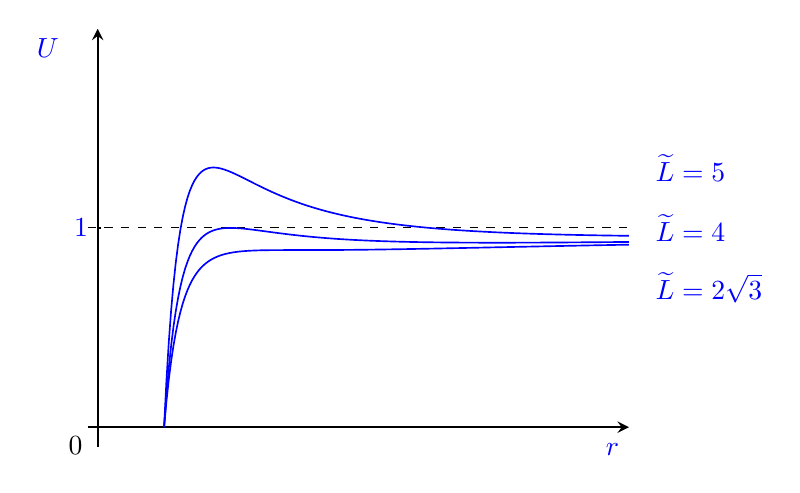
\begin{tikzpicture}[x=0.6pt,y=0.6pt,yscale=120,xscale=20]
%1. 标记重要的点
\coordinate (0) at (0, 0);
\coordinate (ymax) at (0, 2);
\coordinate (ymin) at (0, -0.1);
\coordinate (xmax) at (16, 0);
\coordinate (xmin) at (-0.3, 0);
%2. 绘制基本的坐标轴
\draw[-stealth, thick] (ymin) -- (ymax);
\draw[-stealth, thick] (xmin) -- (xmax);
\draw[dashed] (-0.3,1) -- (16,1);
\node[blue, right=6pt, below] at (-2,2) {$U$};
\node[blue, below=8pt, left] at (16,0) {$r$};
%3. 给 x,y 轴加上刻度
\node[black, left=8pt, below] at (0) {$0$};
\draw[black] (0, 0.5) -- (0.05, 0.5);

\foreach \loc/\y in
	{1/1,}
	{\node[blue, left] at (0,\loc) {$\y$};
	\draw [black, thick] (0,\loc) -- (0.1, \loc);
	\draw [black] (0,\loc+0.5) -- (0.05, \loc+0.5);
	}
%4. 绘制函数图
\draw[blue, semithick, domain=2:16][samples=200] plot(\x, {1-2/\x+16/(\x^2)-32/(\x^3)}) node[blue, right=6pt] at (16, 1){$\widetilde{L}=4$};
\draw[blue, semithick, domain=2:16][samples=200] plot(\x, {1-2/\x+12/(\x^2)-24/(\x^3)}) node[blue, right=6pt] at (16, 0.7){$\widetilde{L}=2\sqrt{3}$};
\draw[blue, semithick, domain=2:16][samples=200] plot(\x, {1-2/\x+25/(\x^2)-50/(\x^3)}) node[blue, right=6pt] at (16, 1.3){$\widetilde{L}=5$};
\end{tikzpicture}
\captionsetup{justification=raggedright, singlelinecheck=false}
\caption{等效势阱。}
\label{等效势阱。}
\end{figure}

在$r$较小的地方,$\widetilde{L}>4$的时候有一峰值大于 1 的势垒,在$r$较大的地方有一势阱(图\ref{等效势阱。}并未绘制出,但随着$r$的增大,$U$会回升至趋向于 1 的情形),此时三类运动都是可能发生的。随着$\widetilde{L}$减小,势垒也在下降,$\widetilde{L}\le4$时,势垒降到$1$以下,散射态消失了。$\widetilde{L}<2\sqrt{3}$时,势垒也消失了,此时也没有势阱的概念了,粒子有很大可能向引力源坠落。实际上,牛顿引力论可以实现半径任意小的圆轨道,但是根据相对论的等效势不可能实现。对于
\begin{equation}
\Phi_{\text{eff}}(r)=\frac{\widetilde{L}^{2}}{2r^{2}}-\frac{GM\widetilde{L}^{2}}{c^{2}r^{3}}-\frac{GM}{r}+\frac12c^{2},
\end{equation}
对$r$求导发现
\begin{equation}
\frac{\mathrm{d}\Phi_{\text{eff}}}{\mathrm{d}r}=\frac{\widetilde{L}^{2}}{r^{4}}(\frac{3GM}{c^{2}}-r)+\frac{GM}{r^{2}}.
\end{equation}
可见对于$r<3GM_{\text{BH}}/c^{2},\dfrac{\mathrm{d}\Phi_{\text{eff}}}{\mathrm{d}r}>0$,无法实现圆轨道。

要实现稳定轨道,首先要求一阶导为零有解
\begin{align}
r^{4}\frac{\mathrm{d}\Phi_{\text{eff}}}{\mathrm{d}r}&=\frac{3\widetilde{L}^{2}GM}{c^{2}}-\widetilde{L}^{2}r+GMr^{2}=0,\\
\Delta{}&=\widetilde{L}^{4}-12\frac{G^{2}M^{2}}{c^{2}}\widetilde{L}^{2}>0,\\
\widetilde{L}&>\frac{2\sqrt{3}GM}{c}.
\end{align}
这也是前文$2\sqrt{3}$的来源。进一步要求二阶导大于零,
\begin{align}
r^{5}\frac{\mathrm{d}^{2}\Phi_{\text{eff}}}{\mathrm{d}r^{2}}&=-\frac{12\widetilde{L}^{2}GM}{c^{2}}+3\widetilde{L}^{2}r-2GMr^{2}>0.\tag{5}\\
r&=\frac{-3\widetilde{L}^{2}\pm\sqrt{(9\widetilde{L}^{4}-96\widetilde{L}^{2}G^{2}M^{2}/c^{2})}}{-4GM},\notag\\
\widetilde{L}&>\frac{2\sqrt3GM}{c},\notag\\
r_{\min}&=\frac{6GM}{c^{2}},r_{\max}=\frac{12GM}{c^{2}}.\tag{6}
\end{align}
因此最小可实现的圆轨道为$\dfrac{6GM}{c^{2}}$.

\subsection{行星的轨道}
理论力学中,行星运动有关的第一积分是
\begin{align}
\frac{\mathrm{d}\varphi}{\mathrm{d}t}&=\frac{L}{r^{2}},\\
\frac12\left(\frac{\mathrm{d}r}{\mathrm{d}t}\right)^{2}&=E+\frac{GM}{r}-\frac{L^{2}}{2r^{2}}.
\end{align}
其中$L$是行星的角动量。消去时间可以得到轨道方程
\begin{equation}
\frac{1}{2}\left[\frac{\mathrm{d}}{\mathrm{d}\varphi}\left(\frac{1}{r}\right)\right]^{2}=\frac{E}{L^{2}}-\frac{1}{2r^{2}}+\frac{GM}{rL^{2}}.
\end{equation}
对$\varphi$微商,得到
\begin{equation}
\frac{\mathrm{d}^{2}}{\mathrm{d}\varphi^{2}}\left(\frac{1}{r}\right)+\frac{1}{r}=\frac{GM}{L^{2}}.
\end{equation}
变量代换$u=\dfrac{GM}{r}$,
\begin{equation}
\frac{\mathrm{d}^{2}u}{\mathrm{d}\varphi^{2}}+u=\left(\frac{GM}{L}\right)^{2}.
\end{equation}
该方程的解是
\begin{equation}
u=\left(\frac{GM}{L}\right)^{2}\left(1+e\cos\varphi\right).
\end{equation}
在极坐标系中根据“到准线和到焦点距离比值为定值”的定义容易发现这是一个椭圆轨道。$e$是偏心率。

相对论动力学可作类似处理,行星轨道满足(继续采用自然单位制)
\begin{align}
\frac{\mathrm{d}t}{\mathrm{d}\tau}&=E\cdot\left(1-\frac{2M}{r}\right)^{-1},\\
\frac{\mathrm{d}\varphi}{\mathrm{d}\tau}&=\frac{\widetilde{L}}{r^{2}},\\
\left(\frac{\mathrm{d}r}{\mathrm{d}\tau}\right)^{2}&=E^{2}-\left(1-\frac{2M}{r}\right)\left(1+\frac{\widetilde{L}^{2}}{r^{2}}\right).
\end{align}
消去固有时$\tau$,可以得到轨道方程
\begin{equation}
\frac{1}{2}\left[\frac{\mathrm{d}}{\mathrm{d}\varphi}\left(\frac{1}{r}\right)\right]^{2}=\frac{E^{2}-1}{2\widetilde{L}^{2}}-\frac{1}{2r^{2}}+\frac{M}{r^{3}}+\frac{M}{r\widetilde{L}^{2}}.
\end{equation}
对$\varphi$作微商,得到
\begin{equation}
\frac{\mathrm{d}^{2}}{\mathrm{d}\varphi^{2}}\left(\frac{1}{r}\right)+\frac{1}{r}=\frac{M}{\widetilde{L}^{2}}+\frac{3M}{r^{2}}.
\end{equation}
做类似的变量代换
\begin{equation}
\frac{\mathrm{d}^{2}u}{\mathrm{d}\varphi^{2}}+u=\left(\frac{M}{\widetilde{L}}\right)^{2}+3u^{2},
\end{equation}
可见其与牛顿理论的区别仅在于$3u^{2}$的修正,对于水星$u\sim10^{-7}$.牛顿解可以看作该非线性微分方程零级近似,代入上式转化成线性方程
\begin{equation}
\frac{\mathrm{d}^{2}u}{\mathrm{d}\varphi^{2}}+u\approx\left(\frac{M}{\widetilde{L}}\right)^{2}+3\left(\frac{M}{\widetilde{L}}\right)^{4}+6\left(\frac{M}{\widetilde{L}}\right)^{4}e\cos\varphi.
\end{equation}
其中略去了$e^{2}$项因为偏心率较小。比较常数项量级可再次简化为
\begin{equation}
\frac{\mathrm{d}^{2}u}{\mathrm{d}\varphi^{2}}+u\approx\left(\frac{M}{\widetilde{L}}\right)^{2}+6\left(\frac{M}{\widetilde{L}}\right)^{4}e\cos\varphi.
\end{equation}
将解分成两个部分$u=u_{1}+u_{2}$,分别对应后两项,可见$u_{1}$就是牛顿解,而通过
\begin{equation}
\frac{\mathrm{d}^{2}u_{2}}{\mathrm{d}\varphi^{2}}+u_{2}=6\left(\frac{M}{\widetilde{L}}\right)^{4}e\cos\varphi
\end{equation}
可以得到
\begin{equation}
u_{2}=3\left(\frac{M}{\widetilde{L}}\right)^{4}e\varphi\sin\varphi.
\end{equation}
略去高于$\left(\dfrac{M}{\widetilde{L}}\right)^{4}$的项,得到水星轨道方程
\begin{align}
u&=u_{1}+u_{2}=\left(\frac{M}{\widetilde{L}}\right)^{2}\left(1+e\cos\varphi+3\left(\frac{M}{\widetilde{L}}\right)^{2}e\varphi\sin\varphi\right)\notag\\
&\approx\left(\frac{M}{\widetilde{L}}\right)^{2}\left\{1+e\cos\left(\left[1-3\left(\frac{M}{\widetilde{L}}\right)^{2}\right]\varphi\right)\right\}.
\end{align}
可见周期不再是$2\pi$,而是
\begin{equation}
T=\frac{2\pi}{1-3\left(\dfrac{M}{\widetilde{L}}\right)^{2}},
\end{equation}
行星要转动
\begin{equation}
\varphi_{n}=2n\pi\left(1+\frac{3M^{2}}{\widetilde{L}^{2}}\right)
\end{equation}
才能回到近日点。相邻两个近日点的方位角之差是
\begin{equation}
\Delta{}\varphi=6\pi\left(\frac{M}{\widetilde{L}}\right)^{2}=6\pi\left(\frac{GM}{c\widetilde{L}}\right)^{2}.
\end{equation}
对于水星,每运动一周,$\Delta{}\varphi=0.1^{\prime\prime}$,累积一世纪积累的进动角是$43^{\prime\prime}$,与观测数据达成了惊人的一致。

\subsection{光线偏折}
类似行星轨道,可以给出光线运动方程(此时采用其他的仿射参量,且$\eta=0$)
\begin{align}
\frac{\mathrm{d}t}{\mathrm{d}\lambda}&=E\cdot\left(1-\frac{2M}{r}\right)^{-1},\\
\frac{\mathrm{d}\varphi}{\mathrm{d}\lambda}&=\frac{\widetilde{L}}{r^{2}},\\
\left(\frac{\mathrm{d}r}{\mathrm{d}\lambda}\right)^{2}&=E^{2}-\left(1-\frac{2M}{r}\right)\frac{\widetilde{L}^{2}}{r^{2}}.
\end{align}
消去仿射参量,后续操作类似行星轨道,可得
\begin{equation}
\frac{\mathrm{d}^{2}u}{\mathrm{d}\varphi^{2}}+u=3u^{2},
\end{equation}
其中$u=\dfrac{GM}{c^{2}r}=\dfrac{GM}{c^{2}}\widetilde{u}$,方程改写成
\begin{equation}
\frac{\mathrm{d}^{2}\widetilde{u}}{\mathrm{d}\varphi^{2}}+\widetilde{u}=\frac{3GM}{c^{2}}\widetilde{u}^{2}.
\end{equation}
可以使用逐次逼近法求解。首先考虑
\begin{equation}
\frac{\mathrm{d}^{2}\widetilde{u}}{\mathrm{d}\varphi^{2}}+\widetilde{u}=0
\end{equation}
的解为零级近似:
\begin{equation}
\widetilde{u}_{0}=R^{-1}\cos\varphi,
\end{equation}
其中$R$是光线到恒星中心的最短距离。上式是一条通过“黄道面”的直线。零级近似代入原方程可求一级近似解
\begin{equation}
\frac{\mathrm{d}^{2}\widetilde{u}_{1}}{\mathrm{d}\varphi^{2}}+\widetilde{u}_{1}=\frac{3GM}{c^{2}R^{2}}\cos^{2}\varphi.
\end{equation}
猜测解形式为$\widetilde{u}_{1}=B\sin^{2}\varphi+B'$,可以定出系数具体值,得到特解:
\begin{equation}
\widetilde{u}_{1}=\frac{GM}{c^{2}R^{2}}\left(1+\sin^{2}\varphi\right).
\end{equation}
因此光线轨道可以写作
\begin{equation}
\widetilde{u}=\widetilde{u}_{0}+\widetilde{u}_{1}=R^{-1}\cos\varphi+\frac{GM}{c^{2}R^{2}}\left(1+\sin^{2}\varphi\right).
\end{equation}
无穷远处 ($\widetilde{u}_{0}=0$) 直线解方位角为$\varphi=\pm\dfrac{\pi}{2}$,一级解可看作添加一个小量$a$,泰勒展开得到无穷远处
\begin{align}
0&=-R^{-1}\sin\alpha+\frac{GM}{c^{2}R^{2}}\left(1+\cos^{2}\alpha\right).\\
a&=\frac{2GM}{c^{2}R}.\\
\Delta{}\theta&=2a=\frac{4GM}{c^{2}R}.
\end{align}
太阳附近数据为$\Delta{}\theta=1.75^{\prime\prime}$,已被日全食时拍摄的星空照片证实。

\printbibliography

\end{document}